\chapter{Results and Conclusions}
\label{ch:res}
In this chapter, we use the forward model to generate some data given an underlying ground truth and then guide the reader through the process of setting up a Bayesian framework and ultimately obtaining the posterior distributions of parameters of interest, such as ozone concentration or pressure and temperature profiles.
We are using a directed acyclic graph (DAG) to visualise hierarchical and correlation structures of a Bayesian model.
Next, we established a choice of prior distributions within our Bayesian model and formulated the posterior distributions.
Based on the linear forward model $\bm{A}_L$, we characterise the marginal posterior for ozone and compare that to the TT approximation.
Then we calculate the mean and the covariance matrix of the full posterior for ozone, which we use to find affine map to approximate the non-linear forward model $\bm{A}_{NL} \approx \bm{M} \bm{A}_{NL}$ (see Sec. \ref{sec:affineMap}).
In Sec. \ref{sec:ComparReg}, we repeat the MTC scheme to provide a posterior distribution of ozone based on the approximate forward model and compare to a regularisation approach and a ground truth.
Additionally, in sec \ref{sec:FullBay}, we extend the hierarchical Bayesian model and MTC scheme to jointly provide conditional posterior distributions of ozone, temperature and pressure.
Here we elaborate on some aspects of prior modelling and on our findings when using a TT to approximate the higher dimensional marginal posterior.
Lastly, we evaluate some errors occurring during the process.
All of programming and analysis is done in Python and the reported computation times correspond to a MacBook Pro from 2019 with a 2.4 GHz quad-core Intel Core i5 processor.
\clearpage
\section{Simulate Data based on a Ground Truth}
We take a ground truth ozone VMR at distinct pressure values generated from some data \cite{MLSdata} of the MLS on the Aura satellite within the Antarctic region and with a peak in high altitude, see Fig. \ref{fig:O3Samp}, which seems to be a typical nighttime profile \cite{Lee2020NightOzone}.

We target Ozone at a frequency of 235.71 GHz, which lies within the region where the MLS observers ozone \cite{livesey2008ozonecarbonmono, waters2006earth}.
The corresponding wave number is $\nu = 7.86\text{cm}^{-1}$.
We recursively calculate the geometric height with the hydrostatic equilibrium equation
\begin{align}
	\frac{\text{d}p}{p} = \frac{- g M}{R^* T} \text{d} h \, ,\label{eq:hydr}
\end{align}
with the acceleration due to gravity
\begin{align}
	g = g_0 \Bigg( \frac{r_0}{r_0 + h} \Bigg) \, ,
\end{align}
where the polar radius pf the earth is $r_0 \approx 6356 \, \text{km}$, the gravitation at sea level is $g_0 \approx 9.81 \text{m}/\text{s}^2$, $R^* = 8.31432 \times 10^{-3} \text{Nm} / \text{kmol} / \text{K}$ and the mean molecular weight of the air is $M = 28.97 \text{kg/kmol}$ \cite{atmosphere1976us}.
This holds up to a geometric height of $86$km, where we ignore a $0.04\%$ non-linear change in $M$ from $80$km to $86$km in geometric altitude.

Following \cite{atmosphere1976us} we form the temperature function
\begin{equation}
	\label{eq:tempFunc}
	T(h) = \adjustbox{max width=0.825\textwidth}{$\begin{dcases*}
			T_0 &, \text{$h  = 0$}\\
			T_0 + a_0 h   &, \text{$0 \leq h < h_{T,1}$}\\
			T_0 + a_0 h_{T,1} &, \text{$h_{T,1} \leq  h < h_{T,2}$}\\
			T_0 + a_0 h_{T,1} + a_1 (h_{T,2}   - h_{T,1})  + a_2 (h   - h_{T,2})  &, \text{$h_{T,2} \leq h < h_{T,3}$}\\
			T_0 + a_0 h_{T,1} + a_1 (h_{T,2}   - h_{T,1})   & \\
			\hphantom{{} T_0 } + a_2 (h_{T,3}   - h_{T,2}) + a_3 (h   - h_{T,3}) &, \text{$h_{T,3} \leq h < h_{T,4}$}\\
			T_0 + a_0 h_{T,1} + a_1 (h_{T,2}   - h_{T,1})  & \\
			\hphantom{{} T_0 }+ a_2 (h_{T,3}   - h_{T,2})  + a_3 (h_{T,4}   - h_{T,3}) + a_4 (h   - h_{T,4}) &, \text{$h_{T,4} \leq h < h_{T,5}$}\\
			T_0 + a_0 h_{T,1} + a_1 (h_{T,2}   - h_{T,1})   & \\
			\hphantom{{} T_0 } + a_2 (h_{T,3}   - h_{T,2}) + a_3 (h_{T,4}   - h_{T,3}) + a_4 (h_{T,5}   - h_{T,4})& \\
			\hphantom{{} T_0 }  + a_5 (h   - h_{T,5}) &, \text{$h_{T,5} \leq h < h_{T,6}$}\\
			T_0 + a_0 h_{T,1} + a_1 (h_{T,2}   - h_{T,1})    &\\
			\hphantom{{} T_0}  + a_2 (h_{T,3}   - h_{T,2}) + a_3 (h_{T,4}   - h_{T,3}) + a_4 (h_{T,5}   - h_{T,4}) &\\ 
			\hphantom{{} T_0} + a_5 (h_{T,6}   - h_{T,5}) + a_6 (h   - h_{T,6})   &, \text{$h_{T,6} \leq h \lesssim  86$}
		\end{dcases*}$}\\
\end{equation}

with gradient and height values provided by \cite{atmosphere1976us}, see Tab. \ref{tab:tempGrad}.
This acts as the ground truth temperature profile, see Fig. \ref{fig:PriorTemp}.
\begin{table}
	\centering
	\begin{tabular}{ |c||c|c|  }
		\hline
		subscript $i$ & geometric height $h_{T,i}$ in km&gradient $a_i$\\
		\hhline{|=||=|=|}
		0& 0 & -6.5\\
		1& 11 & 0\\
		2& 20.1& 1\\
		3& 32.2& 2.8\\
		4& 47.4& 0\\
		5& 51.4& -2.8\\
		6& 71.8& -2\\
		\hline
	\end{tabular}
\caption[Height depending temperature gradients]{Definition of height depending temperature gradients.}
\label{tab:tempGrad}
\end{table}

Then we can compute a data vector $\bm{y} = \bm{A}_{NL} + \bm{\eta} $, with $m = 30$ measurements according to the radiative transfer equation (RTE), see Eq. \ref{eq:RTE} which we solve using the trapezoidal integration rule, determined by the satellite pointing accuracy of $175\text{arc sec}$, see Fig. \ref{fig:TangHCases}.
We assume an atmosphere between $h_{L,1}=7$km and $h_{L,n} = 83.3$km with $n = 45$ equidistant layers.
The height value $h_{L,i}$ for each layer $i = 1,\dots, n$ is defined by the pressure values from \cite{MLSdata} and the hydrostatic equilibrium equation, see Eq. \ref{eq:hydr}.
We calculate the absorption constant $k(\nu,T)$ as in Eq. \ref{eq:absRTE}, following the \textit{HITRAN} database \cite{gordon2022hitran2020}, which provides the line intensity $L(\nu,T_{\text{ref}})$ for the isotopologue $\prescript{16}{}{\text{O}}_3$ with the AFGL Code 666.
This gives us a non-linear forward model matrix $\bm{A}_{NL} = \bm{A}(\bm{x}, \bm{p}, \bm{T}) \in \mathbb{R}^{m \times n}$, where $\bm{x}\in \mathbb{R}^{n}$ is vector related to the ozone VMR, $\bm{p}\in \mathbb{R}^{n}$ is the vector describing the pressure values and $\bm{T}\in \mathbb{R}^{n}$ the temperature values.

Lastly we add normally distributed $\bm{\eta} \sim \mathcal{N}(0,\gamma^{-1} \bm{I})$ noise so that the SNR is $150$, see Eq. \ref{eq:SNR}, similar to \cite{Froidevaux2008snrozone}, where a signal with a maximal spectral intensity of around $100\text{K}$ and a noise range of $0.4$ to $1.6\text{K}$ is reported.
We note that the methods used in this thesis will work with different SNRs or other frequencies.

When we plot the data in Fig. \ref{fig:DataPlot}, we see that, as mentioned in Section \ref{sec:SVD}, the data is noise-dominated in higher altitudes.
\begin{figure}[th!]
	\centering
	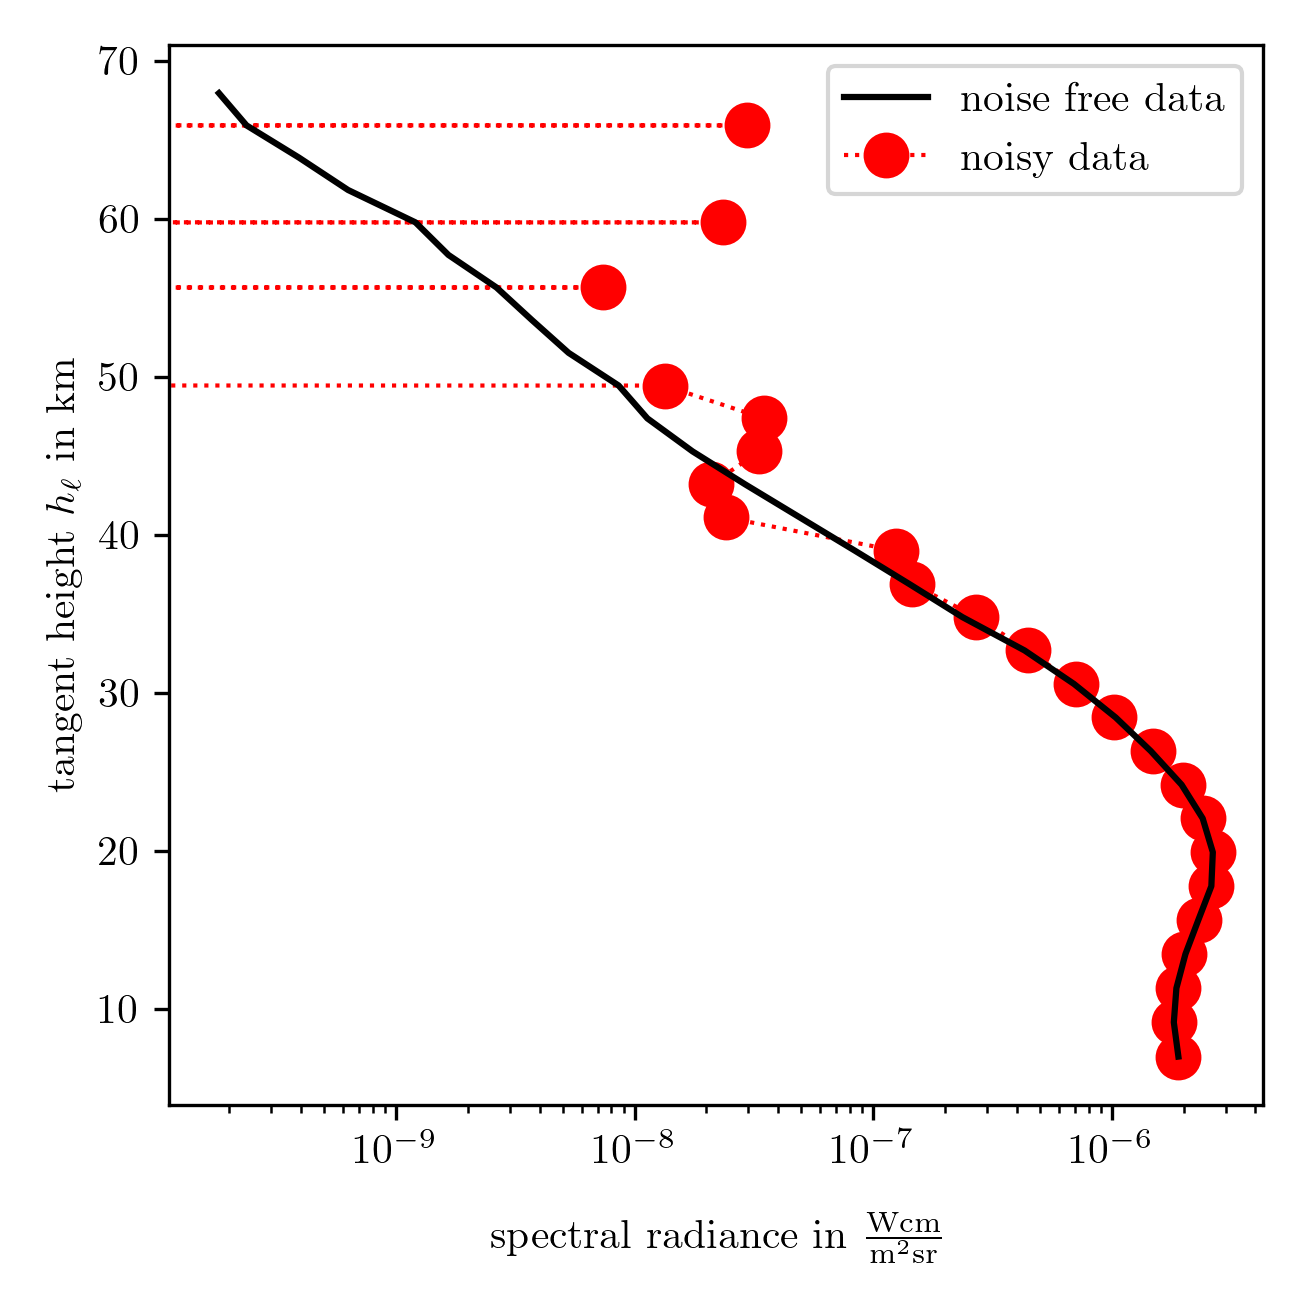
\includegraphics{DataPlot.png}
	\caption[Logarithmic plot of data points at different tangent height.]{Logarithmic plot of data points at different tangent height. Note that negative values are not appearing, and we see that the noise is dominating at high altitudes.}
	\label{fig:DataPlot}
\end{figure}
Now, given the data, we like to determine the posterior distributions over ozone $\bm{x}$, pressure $\bm{p}$ and temperature $\bm{T}$ at different heights.
\clearpage


\section{Hierarchical Bayesian Framework for Ozone}
\label{sec:BayModelO3}
\begin{figure}[htb!]
	\centering
	\begin{tikzpicture}
		%box/.style = {draw, thick, minimum width=2.5cm, minimum height=1cm},
		every edge/.style = {draw, -latex, thick} % <---
		\node[roundnode2] at (-4,6.5) (Q)     {$\bm{Q}$};
		\node[roundnode2] at (-2.5,5) (x)     {$\bm{x}$};
		\node[align=center] at (-1,4) (A)    {$\bm{A}$};
		\node[roundnode2] at (-1,2.5) (u)    {$\Omega$};
		\node[rectnode] at (-1,1) (y)    {$\bm{y}$};
		\node[roundnode2] at (-2.5,2.5) (e)    {$\bm{\eta}$};
		\node[roundnode2] at (-6.5,6.5) (S)    {$\bm{\Sigma}$};
		\node[roundnode2] at (-8,8) (s)    {$\gamma$};
		\node[roundnode2] at (-5.5,8) (d)    {$\delta$};
		
		\node[roundnode2] at (-8,10) (shyp)    {$\bm{\theta}_{\gamma}$};
		\node[roundnode2] at (-5.5,10) (dhyp)    {$\bm{\theta}_{\delta}$};
		%Lines
		\draw[->, very thick] (S) -- (e);
		\draw[->, mydotted, very thick] (s) -- (S);
		\draw[->, mydotted, very thick] (e) -- (y);
		\draw[->, very thick] (u.south) -- (y);
		\draw[->, mydotted, very thick] (A) -- (u);
		\draw[->, mydotted,  very thick] (x) -- (A.west);
		\draw[->, very thick] (shyp) -- (s);
		\draw[->, very thick] (dhyp) -- (d);
		
		
		\draw[->, mydotted, very thick] (d) -- (Q); 
		
		\draw[->, very thick] (Q) -- (x); 
		%\node[align=center] at (0,4) (f3) {$= \bm{A}$};
		%\node[align=center] at (0.25,3.95) (f3) {$\approx \bm{M A}_L$};
		\node[align =center] at (-2,8) (T1) {marginal posterior \\ over hyper-parameters \\ $\pi(\delta,\gamma  | \bm{y})$};
		\node[align =center] at (0,5) (T2) {conditional posterior \\ $\pi( \bm{x} | \delta,\gamma, \bm{y})$ };
		
		%\node[align =center] at (-2.5,10) (T3) {hyper-prior distributions \\ $\pi( \delta, \gamma)$ };
		
		\node[fit=(s)(d),draw,dotted,black, rounded corners] {};
		\draw[->,dotted] (y) edge[bend right=90] (T1);  
		\draw[->,dotted] (T1) -- (T2); 

	\end{tikzpicture} 
	\caption[Directed acyclic graph for ozone retrieval and MTC scheme.]{DAG for visualisation of hierarchical modelling and measuring process of ozone including the MTC scheme. The hyper-parameter $\gamma$ deterministically (dotted line) sets the noise covariance $\bm{\Sigma} = \gamma^{-1}\bm{I}$ and hence the random (solid line) noise vector $\bm{\eta} \sim \mathcal{N}(0, \gamma^{-1}\bm{I})$.
	The hyper-parameter $\delta$ determines (dotted line) the prior precision matrix $\bm{Q} = \delta \bm{L}$ for the normally distributed (solid line) prior $\bm{x}| \delta \sim \mathcal{N}(0, \delta \bm{L})$, where $\bm{L}$ is a graph Laplacian, see Eq. \ref{eq:GLapl}.
	The hyper-prior distributions (solid line) $\pi(\delta, \gamma)$ are defined by $\bm{\theta}_{\gamma}$ and $\bm{\theta}_{\delta}$.
	Through the linear forward model $\bm{A}$ we generate a space of all measurable noise free data $\bm{A}\bm{x}$ from which we randomly observe a data set $\bm{y}$ including some added noise $\bm{\eta}$.
	Within the MTC scheme we evaluate the marginal posterior over the hyper-parameters $\pi(\gamma, \delta | \bm{y})$ first and then the conditional posterior $\pi(\bm{x}|\delta,\gamma,\bm{y})$. This breaks the correlation structure of $\bm{x}$ and $\delta$ and $\gamma$, and allows to evaluate the marginal posterior independent of $\bm{x}$.}
	\label{fig:DAGO3}
\end{figure}
In this section, we setup the hierarchically-ordered linear-Gaussian Bayesian framework to determine the ozone posterior distribution, conditioned on ground truth temperature and pressure.
Where for now we define the forward model matrix $\bm{A} = \bm{A}_L$ and define the distributions of that Bayesian model, similarly to a regularisation approach, as:
\begin{subequations}
	\begin{align}
		\bm{y} |  \bm{x},\gamma,\delta  &\sim \mathcal{N}(\bm{A} \, \bm{x}, \gamma^{-1} \bm{I}) \label{eq:likelihoodAppl} \\
		\bm{x}| \delta  &\sim \mathcal{N}(\bm{0}, (\delta \bm{L})^{-1} ) \label{eq:priorXAppl} \\
		\delta  &\sim \Gamma(\alpha_{\delta} = 1, \beta_{\delta} = 10^{-35})\label{eq:priorDelAppl} \\
		\gamma  &\sim \Gamma(\alpha_{\gamma} =1, \beta_{\gamma} = 10^{-35})\label{eq:priorGamAppl} \, .
	\end{align} 
	\label{eq:O3BayMode}
\end{subequations}
Assuming Gaussian noise $\bm{\eta} \sim \mathcal{N}(0, \gamma^{-1} \bm{I})$, the likelihood function is a normal distributions with mean $\bm{A} \bm{x}$ and covariance matrix $\gamma^{-1} \bm{I}$.
We define the normal prior-distribution $\pi(\bm{x}|\delta)$, with zero mean and precision matrix $\delta \bm{L}$, where $\delta$ is a smoothness hyper-parameter and $\bm{L}$ is the second order discrete derivate operator (see Eq. \ref{eq:GLapl}).
Here the hyper-prior distributions $\pi(\delta)$ and $\pi(\gamma)$ are gamma distributions with shape $\alpha$ and rate $\beta$.

We can visualise this hierarchical structure and the correlations in between different hyper-parameters and parameters through a DAG.
The hyper-parameter $\gamma$ sets the noise covariance deterministically (dotted line), but is it self statistically (solid line) defined by the hyper-prior distribution $\pi(\gamma)$.
In this case $\theta_{\gamma}$ determines the hyper-prior distribution $\pi(\gamma)$, and similarly $\theta_{\delta}$ for $\pi(\delta)$, which then deterministically sets the prior precision $\bm{Q}$.
In our case, $\delta$ accounts for smoothness of the ozone profile.
Then $\bm{A}\bm{x}$ determines the space of all measurable noise-free data sets $\Omega$, through the linear forward model, from which we observe a data set $\bm{y}$ including some noise $\bm{\eta}$.
From that data we then "reverse the arrows" to determine the posterior distribution over the parameter $\bm{x}$.
Since noise is a random process with a defined distribution, the posterior distribution $\pi(\bm{x}|\bm{y})$ is well defined.
Usually, due to underlying correlation structures, evaluating this posterior poses a signifiant challenge, here the MTC scheme provides the marginal posterior $\pi(\delta, \gamma | \bm{y})$ first and then the conditional posterior $\pi(\bm{x}|\delta, \gamma,\bm{y})$.
%Since the forward model described in Ch. \ref{ch:formodel} is weakly non-linear we will set up a linear Bayesian hierarchical framework first based on the linear forward model $\bm{A}_L$ and then later the approximated version $\bm{A}_{NL}\bm{M} \bm{A}_L$.
%Furthermore, the noise is normally distributed, so we establish a linear-Gaussian Bayesian hierarchical framework, aiming to recover an ozone profile and a pressure over temperature profile.
%In doing so, we first draw a directed acyclic graph (DAG) to visualise the measurement and modelling process and determine hyper-parameters and correlations between parameters.
%Then we define prior distributions over all parameters as well as a likelihood function so that we can formulate the posterior distribution.

%In this section, we choose the prior distributions and describe the approach to evaluate the posterior distribution for ozone $\pi(\delta, \gamma, \bm{x}|\bm{y})$, including the noise hyper-parameter $\gamma$.
% we define a linear-Gaussian Bayesian hierarchical model, see Sec. \ref{subsec:LinBay},
%\begin{subequations}
%	\begin{align}
%		\bm{y} |  \bm{x}, \gamma &\sim \mathcal{N}(\bm{A} \bm{x}, \gamma^{-1} \bm{I}) \label{eq:likelihood} \\
%		\bm{x} |  \delta &\sim \mathcal{N}(\bm{0}, (\delta \bm{L})^{-1}) \label{eq:xPrior} \\
%		\delta, \gamma &\sim \pi(\delta, \gamma) \label{eq:gammaPrior},
%	\end{align}
%	\label{eq:O3BayMode}
%\end{subequations}
%with a normally distributed likelihood $\pi(\bm{y} |  \bm{x}, \gamma)$ including the forward model matrix $\bm{A}$ and prior distributions $\pi(\bm{x} |  \delta)$ and $\pi(\delta, \gamma)$, the noise covariance matrix $\gamma^{-1} \bm{I}$, the prior precision matrix $\delta \bm{L}$ and the prior mean set to zero, as in ~\cite{fox2016fast}.
%The chosen Bayesian model is very similar to the regularisation approach, since we like to show that we receive much more meaningful results compared to a single regularisation solution.

\subsection{Prior Modelling}
\label{subsec:PriorModelO3}
To complete the Bayesian framework, we have to define prior distributions over the hyper-parameters and parameters.
Ideally, we define the prior distributions as uninformative as possible, and include functional dependencies and physical properties.

By choosing a normally distributed prior $\pi(\bm{x}|\delta)$ with zero mean and no other restrictions, we can already see that our model is not taking into account that ozone values can not be negative.
As already mentioned, we set the precision matrix of that prior distribution to
\begin{align}
	\delta \bm{L} =
	\delta
	\begin{bmatrix}
		2 & -1 & & &  \\
		-1 & 2 & -1 & &   \\
		& \ddots & \ddots & \ddots &\\ 
		& & -1 & 2 & -1  \\
		& & & -1 & 2 
	\end{bmatrix} 
	\label{eq:GLapl} 
\end{align}
which is a 1-dimensional Graph Laplacian as in \cite{wang2015graphs,fox2016fast} with Dirichlet boundary condition.
This matrix will also act as the regulariser later in the Regularisation section, see Sec. \ref{sec:regularise}.
We reduce the dimension of $\bm{x}$ from $45$ to $34$ by discarding every second ozone VMR over a height of $\approx47$km.
Doing that, while not changing $\bm{L}$, we effectively induce a larger correlation between points at higher altitude.
We plot the corresponding prior ozone profiles according to $\bm{x}\sim \mathcal{N}(0, (\delta \bm{L})^{-1})$ in Fig. \ref{fig:O3Prior}.

For $\delta$ and $\gamma$ we pick relatively uninformative gamma distributions so that $\gamma \sim \mathcal{T}(\bm{\theta_{\gamma}}) \propto \gamma^{\alpha_\gamma -1 } \exp{( -\beta_\gamma \gamma) } $ and $\delta \sim \mathcal{T}(\bm{\theta_{\delta}})$, where $\bm{\theta_{\gamma}} = \{  \alpha_\gamma, \beta_\gamma\}  = \{ \alpha_\delta ,\beta_\delta\} = \bm{\theta_{\delta}} = (1,10^{-35})$, see Fig. \ref{fig:MargPostHistTT}, similar to \cite{fox2016fast}.
Those gamma distributions have another advantage when using a MWG algorithm to sample from the marginal posterior distribution $\pi(\delta, \gamma | \bm{y})$.
In doing so, we introduce the regularisation parameter $\lambda = \delta / \gamma $ so that $\pi(\gamma | \lambda, \bm{y}) \sim \mathcal{T}(\cdot)$ is a gamma distribution and easy to sample from.
\clearpage
\subsection{Posterior Distribution -- linear Model}
\label{sec:FirstO3Post}
As explained in Sec. \ref{subsec:LinBay} we factorise the posterior
\begin{align}
	\pi( \bm{x}, \delta, \gamma| \bm{y}) \propto \pi(\bm{y}| \bm{x},\delta,\gamma) \pi( \bm{x},  \delta,\gamma)
\end{align}
into 
\begin{align}
	\pi( \bm{x},  \delta,\gamma| \bm{y}) =\pi( \bm{x}| \delta,\gamma, \bm{y})\pi( \delta,\gamma | \bm{y})
\end{align}
the marginal posterior $\pi(\delta ,\gamma| \bm{y})$ and conditional posterior $\pi( \bm{x}| \delta,\gamma, \bm{y})$ (see Eq. \ref{eq:MTC}).
%Fox and Norton call this method the marginal and then conditional method (MTC) \cite{fox2016fast}, where we break the correlation structure between $\bm{x}$ and $\gamma, \delta$ as illustrated in Fig. \ref{fig:RueHeld} by marginalising over $\bm{x}$.
As discussed in sec. \ref{subsec:LinBay}, for the linear-Gaussian case, $\bm{x}$ cancels in the marginal posterior over the hyper-parameters.
Following the MTC scheme, we characterise the marginal posterior first and \textit{then} the conditional posterior of $\pi(\bm{x} | \delta,\gamma)$.

\subsubsection{Marginal Posterior}
\label{subsec:FirstMTC}
Consequently, for the hierarchical model specified in Eq.~\ref{eq:O3BayMode}, the marginal posterior distribution over the hyper-parameters is given by
\begin{align}
	\pi( \lambda,\gamma  | \bm{y}) \propto &  \lambda^{n/2 + \alpha_{\delta}-1} \gamma^{m/2 + \alpha_{\delta} + \alpha_{\gamma}-1}   \exp{ \Bigl\{ - \frac{1}{2} g ( \lambda) - \frac{\gamma}{2} f ( \lambda) - \beta_{\delta} \lambda  \gamma - \beta_{\gamma} \gamma \Bigr\}},
	\label{eq:MargPostAppl}
\end{align}
with the introduced regularisation parameter $\lambda = \delta / \gamma$, and
\begin{subequations}
	\label{eq:fandg}
	\begin{align}
		&f ( \lambda) = \bm{y}^T \bm{y} - (\bm{A}^T \bm{y})^T (\bm{A}^T  \bm{A} + \lambda \bm{L})^{-1} (\bm{A}^T \bm{y})  \label{eq:fAppl} \, ,  \\
		&\text{and } g(\lambda) = \log \det (\bm{A}^T  \bm{A} + \lambda \bm{L}) \label{eq:gAppl} \, .
	\end{align}
\end{subequations}
Note that, when changing variables from $\delta = \lambda \gamma$ to $\lambda$ the hyper-prior distribution changes to $\pi(\lambda) \propto \lambda^{\alpha_{\delta}-1} \gamma^{\alpha_{\delta}} \exp{(- \beta_{\delta} \lambda  \gamma)} $, due to $\text{d}\delta / \text{d} \lambda = \gamma$.
\begin{figure}[th!]
	\centering
	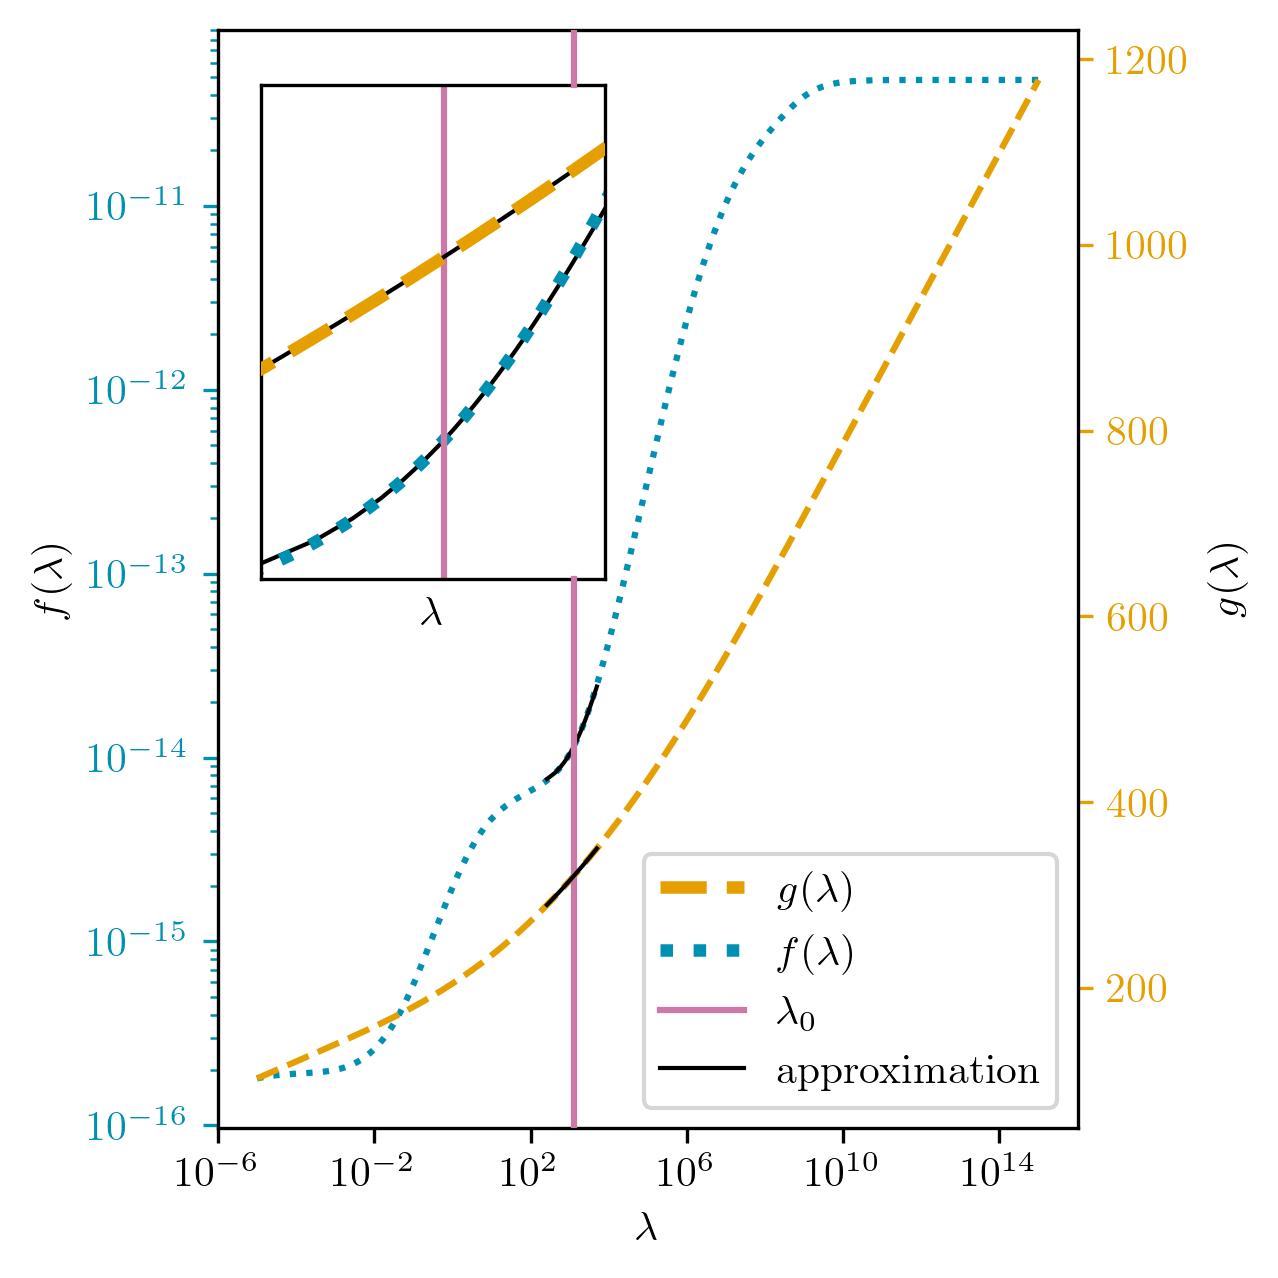
\includegraphics{f_and_g_phd.png}
	\caption[Plot of the functions $f(\lambda)$ and $g(\lambda)$ for marginal posterior.]{Plot of the functions $f(\lambda)$ and $g(\lambda)$ from the marginal posterior for a wide range of $\lambda = \delta / \gamma$. We plot the third-order Taylor series in black around the mode of the marginal posterior (vertical line) for the sampling range of $\lambda$ within the MWG algorithm.}
	\label{fig:fandg}
\end{figure}
Most of the computational effort, for each function evaluation of the marginal posterior in Eq. \ref{eq:MargPostAppl}, lies in the calculation of $f(\lambda)$ in Eq. \ref{eq:fAppl} and $g(\lambda)$ in Eq. \ref{eq:gAppl}.
In  Fig. \ref{fig:fandg} we see that $f(\lambda)$ and $g(\lambda)$ are well behaved within the region of interest and approximate $f(\lambda) \approx \tilde{f}(\lambda)$ with a 3rd order Taylor series around the mode $\lambda_0$ of $\pi(\lambda, \gamma | \bm{y})$.
We also note that $\tilde{g}(\lambda) \approx g(\lambda)$ behaves linearly around $\lambda_0$ in the log-space.
The approximations are implicitly given by
\begin{align}
	f^{(r)}& (\lambda_0)= (-1)^{r+1} (\bm{A}^T \bm{y})^T (\bm{B}_0^{-1} \bm{L})^r \bm{B}_0^{-1} \bm{A}_L^T \bm{y} \label{eq:ftay}  \\
	\text{and } & \log{ \tilde{g}(\lambda)} = (\log{\lambda} - \log{\lambda_{0}})  \frac{ \log{g(\lambda_{\text{max}})} - \log{g(\lambda_{0})} }{\log{\lambda_{\text{max}}} - \log{\lambda_{0}} } + \log{ g(\lambda_{0})} 
	\label{eq:gtay}
\end{align} 
with $\bm{B}_0 = \bm{A}^T  \bm{A} + \lambda_0 \bm{L}$.
We plot the approximations
\begin{subequations}
	\label{eq:fandg}
	\begin{align}
		&\tilde{f} ( \lambda) = \sum^3_{r=0} 	f^{(r)}(\lambda_0) (\lambda-\lambda_0)^r  \label{eq:fAprox} \, ,  \\
		&\text{and } \tilde{g} (\lambda) = \exp \log{\tilde{g}(\lambda)}  \label{eq:gAprox} \, ,
	\end{align}
\end{subequations} in Fig. \ref{fig:fandg} and elaborate on the approximation errors in Sec \ref{sec:fgErros}.
Note that usually a Taylor series includes a factor $(r!)^{-1}$, in this case it cancels in $f^{(r)}(\lambda_0)$, see \cite{fox2016fast}.

\paragraph{Error due to Approximation of f and g}
\label{sec:fgErros}
We report an maximum approximation error in between f and g
For 2nd order taylor 3rd tayle and 4th order taylor

then we neglect ther erro in g beacus ethabsolute in f and g are
and propagtion error in marginal is due to f is realtive RMS and the maximum error is ...


When approximating the functions $f(\lambda)$ and $g(\lambda)$, we find that the 3rd-order Taylor series of $f(\lambda)$ and a linear approximation of $g(\lambda)$ in log-space give the smallest error.
The Taylor series truncation error of $f(\lambda)$ is bounded by the fourth order Taylor series $E_f = \underset{\lambda}{\text{arg max}\,} f^{(4)}(\lambda_0)/ 4! \, (\lambda - \lambda_{0} )^4$ and corresponds to an relative error bounded by $20\%$.
Since the maximum absolute error of the approximation $\underset{\lambda}{\text{arg max}\,}|\tilde{g}(\lambda) - g(\lambda) | \approx 1$ corresponds to an relative error of approximately $0.3\%$ and is small compared to $E_f \approx 1e8$ we ignore the approximation error of $g(\lambda)$.
Then the maximum relative propagation error $\underset{\lambda, \gamma}{\text{arg max}\,} 0.5 \gamma  E_f / \log{\pi{(\lambda ,\gamma | \bm{y})}} $ is bound by approximately $5\%$.

\paragraph{Sample from Marginal Posterior}
Using these approximation we can either utilise a TT approximation of the marginal posterior, see Sec. \ref{subsec:TTMarg}, over a predefined grid and calculate the marginals $\pi(\gamma|\bm{y})$ and $\pi(\lambda|\bm{y})$, or employ a Metropolis within Gibbs (MWG) sampler to sample from $\pi(\lambda,\gamma|\bm{y})$, see sec. \ref{subsec:MWG}.
More specifically, we implement a Metropolis random walk on
\begin{align}
	\label{eq:margApplCondGam}
	\pi(\lambda | \gamma, \bm{y}) &\propto \lambda^{n/2 +\alpha_{\delta}-1} \exp{\Bigl\{ - \frac{1}{2} g ( \lambda) - \frac{\gamma}{2} f ( \lambda) - \beta_\delta \gamma \lambda \Bigr\}}.
\end{align} 
We accept or reject a proposal $\lambda^{\prime} \sim \mathcal{N}(0, \sigma_{\lambda})$ according to the acceptance ratio in log space
\begin{align} 
	\log \left\{ \frac{\pi(\lambda^{\prime} | \gamma^{(k)}, \bm{y})  }{\pi(\lambda^{(k)}| \gamma^{(k)}, \bm{y})}  \right\} 
	= \log  \{\pi(\lambda^{\prime} | \gamma^{(k)}, \bm{y} ) \}  -\log  \{ \pi(\lambda^{(k)}| \gamma^{(k)}, \bm{y}) \} \\
	= \frac{n}{2} (\log\{\lambda^{\prime}\} - \log\{\lambda^{(k)}\} ) + \frac{1}{2} \Delta g + \frac{\gamma^{(k)}}{2} \Delta f  + \beta_\delta \gamma^{(k)} \Delta \lambda  \, ,
\end{align}
where $\Delta \lambda = \lambda^{\prime} - \lambda^{(k)} $ and  $\Delta f \approx \tilde{f}(\lambda^\prime) - \tilde{f}(\lambda^{(k)}) = \sum^3_{r = 1} f^{(r)} (\lambda_0) (\Delta \lambda^\prime - \Delta \lambda^{(k)})^r $, with  $\Delta \lambda^{\prime} = \lambda^\prime - \lambda_0 $ and $\Delta \lambda^{(k)} =  \lambda^{(k)} - \lambda_0$.
Similarly we approximate $\Delta g \approx \tilde{g}(\lambda^{\prime}) -\tilde{g}(\lambda^{(k)})$.
Lastly, we do a Gibbs step on
\begin{align}
	\gamma^{(k+1)} |  \lambda^{(k+1)}, \bm{y} &\sim \Gamma \bigg( \frac{m}{2} + \alpha_\delta + \alpha_\gamma, \frac{1}{2} f (\lambda^{(k+1)}) + \beta_\gamma + \beta_\delta \lambda^{(k+1)} \bigg)\label{eq:GibbsStep}
\end{align} 
to generate marginal posterior samples $(\lambda, \gamma)^{(1)}, \dots, (\lambda, \gamma)^{(N)} \sim  \pi(\lambda, \gamma| \bm{y})$.
%
%We find the mode at the minimum of  $-\log\{ \pi(\lambda, \gamma | \bm{y}) \}$  using \texttt{scipy.optimize.fmin} function and limit the number of function evaluation to 25 and use Cholesky back and forward substitution to calculate values of $g(\lambda)$ and $f(\lambda)$.
%Additionally, we calculate $\bm{B}_0^{-1} \bm{L} $ and  $\bm{B}_0^{-1}  \bm{A}_L^T \bm{y}$ once more at $\lambda_0$ and plot the Taylor approximation within the sampling region in Fig. \ref{fig:fandg}.
%\subsection{Posterior distributions with Linear model for Ozone -- MTC}
%\label{sec:firstMTC}
%In this section we calculate the posterior marginal and then conditional (MTC) posterior distribution for ozone conditioned on the ground truth temperature and pressure profiles using the linear forward model $\bm{A}_L$.
%This is faster then the other way round (finding temperature over pressure conditioning on ozone) and temperature and pressure are well defined within the atmosphere so it is easier to just condition on a temperature and pressure profile out of a text book.
%We employ a so-called Metropolis within Gibbs (MWG) algorithm on the marginal posterior as summarised in the algorithmic Box \ref{alg:margPost} or use a Tensor-Train (TT) approximation to calculate marginal posterior values.
%Then we can either sample from the conditional posterior using the randomise then optimise (RTO) method or calculate conditional mean and variance using quadrature.
%The DAG in Fig. \ref{fig:DAGO3} visualises that process and we can show explicitly that we group the hyper-parameters $\delta, \gamma$ together to determine the marginal posterior $\pi(\gamma, \delta | \bm{y})$.
%Here $\gamma$ , the noise parameter, determines the noise precision $\bm{\Sigma} = \gamma ^{-1} \bm{I}$ and $\delta$, the smoothness parameter, the precision matrix $\bm{Q} = \delta \bm{L}$ of the prior distribution for $\bm{x}$.
%Then conditioned on the hyper-parameters the conditional posterior $\pi( \bm{x} |\gamma, \delta, \bm{y})$ gives the distribution of posterior ozone profiles.
%Note that we use the linear model $A_L$ here as we do not have an approximation to the non-linear model yet and all prior distributions are defined in Table \ref{tab:priors}.
%The full posterior $\pi(\bm{x},\gamma, \delta | \bm{y}) =  \pi(\bm{x}|\gamma, \delta ,\bm{y}) \pi(\gamma, \delta | \bm{y}) $ is given by multiplication of the marginal and conditional posterior densities. 
%\begin{align}
%	\bm{x} |  \bm{\theta}, \bm{y} \sim \mathcal{N} \Big(
%	\underbrace{\bm{\mu} + \left( \bm{A}^T \bm{\Sigma}^{-1} \bm{A} + \bm{Q} \right)^{-1} \bm{A}^T \bm{\Sigma}^{-1} (\bm{y} - \bm{A} \bm{\mu})}_{\bm{\mu}_{\bm{x} |  \bm{\theta}, \bm{y}}},
%	\underbrace{ \left( \bm{A}^T \bm{\Sigma}^{-1} \bm{A} + \bm{Q} \right)^{-1} }_{\bm{\Sigma}_{\bm{x} |  \bm{y}, \bm{\theta}}}
%	\Big) \, ,
%\end{align}
%is normal distribution and we compute weighted expectations, as in Eq.~\ref{eq:MargExpPos}, of the conditional mean and covariance matrix, where the weights are given by $\pi(\bm{\theta} | \bm{y})$. 
%Note that both the noise covariance $\bm{\Sigma} = \bm{\Sigma}(\bm{\theta})$ and the prior precision matrix $\bm{Q} = \bm{Q}(\bm{\theta})$ depend on the hyper-parameters $\bm{\theta}$.

The mode $( \lambda_{0}, \gamma_0 )$ of $\pi(\lambda,\gamma| \bm{y})$ is provided by the \texttt{scipy.optimize.fmin} function and we approximate $f(\lambda)$  and $g(\lambda)$ accordingly.
In doing so, we compute the vector $\bm{B}_0^{-1}\bm{A}^T\bm{y} = (\bm{A}^T\bm{A} + \lambda_0 \bm{L})\bm{A}^T\bm{y} $, the matrix $\bm{B}_0^{-1}\bm{L}$ and the determinant in $g(\lambda)$ using Cholesky decomposition.
Then we approximate $f(\lambda)$ with a 3rd order Taylor series and $g(\lambda)$ with a linear approximation in the log-space, where for the approximation in $g(\lambda)$ we set $\lambda_{\text{max}}$ to the maximum value of $\lambda$ on the TT-grid (see next Paragraph).
To sample from $\pi( \lambda,\gamma| \bm{y})$ we employ the MWG algorithm, see Alg. Box \ref{alg:MwG}, initialised at the mode $(\lambda^{(0)} , \gamma^{(0)}  ) = ( \lambda_{0} , \gamma_{0}  )$ and take $N = 10000$ plus $N_{\text{burn-in}} = 100$ steps in approximately $0.3$s.
The standard deviation of the normal proposal distribution is set to $\sigma_{\lambda} = 0.8 \lambda_0$ so that the acceptance rate is $\approx 0.5$ as suggested in \cite{robertsLecNot}.
The samples are plotted in Fig. \ref{fig:ScatterPlotTT} as a 2D scatter plot, as well as the trace of the MWG to show ergodicity.
We calculate the integrated autocorrelation time (IACT) with the Python implementation of \cite{wolff2004monte}, provided by \cite{drikHesse}, which gives us $\tau_{\text{int}, \gamma} = $ and $\tau_{\text{int}, \delta} = $, see Fig. \ref{fig:IATCLamLin} and Fig. \ref{fig:IATCGamLin}.
\begin{figure}[h!]
	\centering
	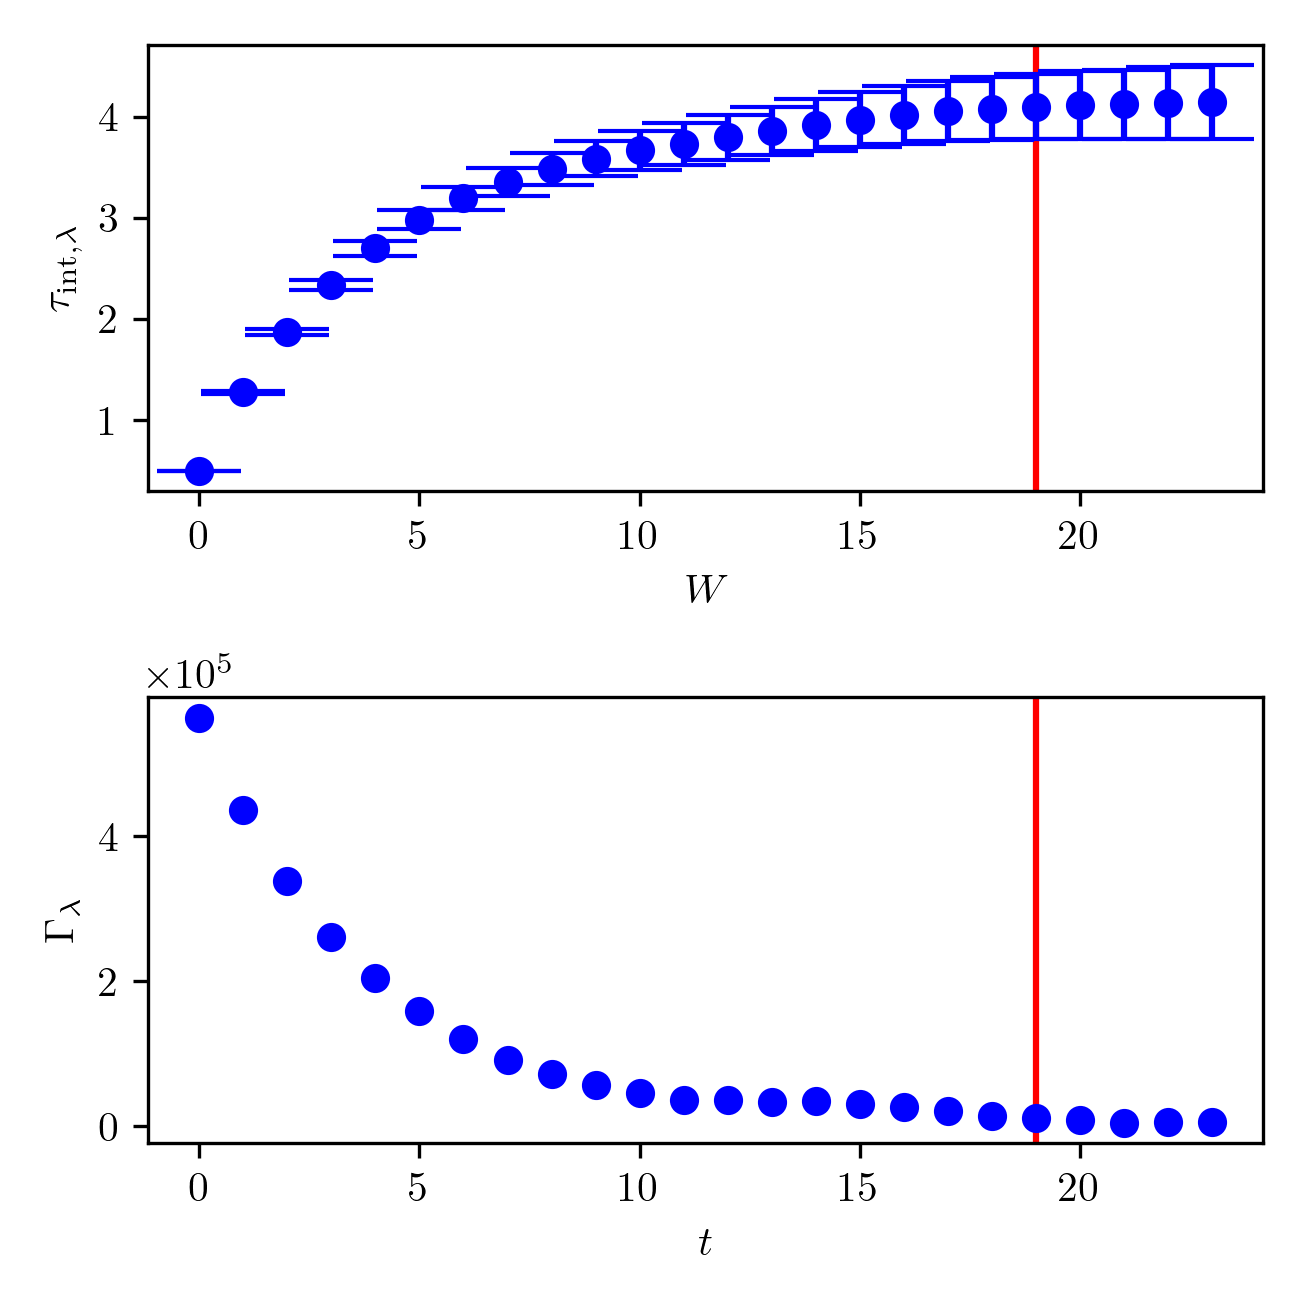
\includegraphics{UwerrTauIntFirstO3lam.png}
	\caption[IATC of $\lambda$ samples from $\pi(\gamma, \lambda| \bm{y})$, for linear model.]{Here the autocorrelation function $\Gamma_{\lambda}$ at different lags W is plotted as well as the IATC $\tau_{\text{int},\lambda}$ for the samples from $\pi(\gamma, \lambda| \bm{y})$ based on the linear forward model.}
	\label{fig:IATCLamLin}
\end{figure}
\clearpage

\paragraph{TT Approximation of Marginal Posterior}
We approximate the square root of marginal posterior on a predefined univariate grid, where $\gamma = [ 0.25 \times 10^{15}, 5.5 \times 10^{15}]$ and $\lambda = [ 100, 5000]$.
We set the number of grid points to $n = 20$ and the number of ranks $r = 5$, which we keep constant.
Since we do not approximate $\sqrt{ \pi( \lambda, \gamma| \bm{y}) }$ in the log-space we introduce a "normalisation constant" $c = 340$. This avoids underflow so that the values $\sqrt{\pi( \lambda,\gamma| \bm{y})} = \exp \{ 0.5 \log  \pi(\lambda,\gamma | \bm{y}) + c \} $ are within computer precision.
Then we initialise the \texttt{tt.cross.rectcross.rect\_cross.cross} function, based on the TT cross algorithm in \cite{OSELEDETS2010TTCross,Dolgov2018TTCross}, from the Python package \texttt{ttpy} \cite{Oseledets2018ttpy}, with a random tensor and do 1 sweep to obtain a TT approximation of $\pi( \lambda,\gamma| \bm{y})$.
This takes about $0.1s$ for $400$ function evaluations.
Then we compute the marginals $\pi(\lambda| \bm{y})$ and $\pi(\gamma| \bm{y})$ as described in Sec. \ref{subsec:TTMarg}.
In doing so we calculate the coefficient tensor $\bm{B}$ and $\bm{B}_{\text{pre}}$ as in Prop. \ref{prob:backMarg} and \ref{prob:ForMarg}, where we set $\xi = 1 / \uplambda (\mathcal{X})$ and $\uplambda(x) = 1$, so that for Cartesian basis $\bm{M}_k = \text{diag}(\uplambda_k(\mathcal{X}_k))$ in Eq. \ref{eq:MassMat}.
We plot the TT approximation as a colour map on top of the obtained samples in the scatter plot in Fig. \ref{fig:ScatterPlotTT}.
We report a RMS error over the whole grid of ...
\begin{figure}[h!]
	\centering
	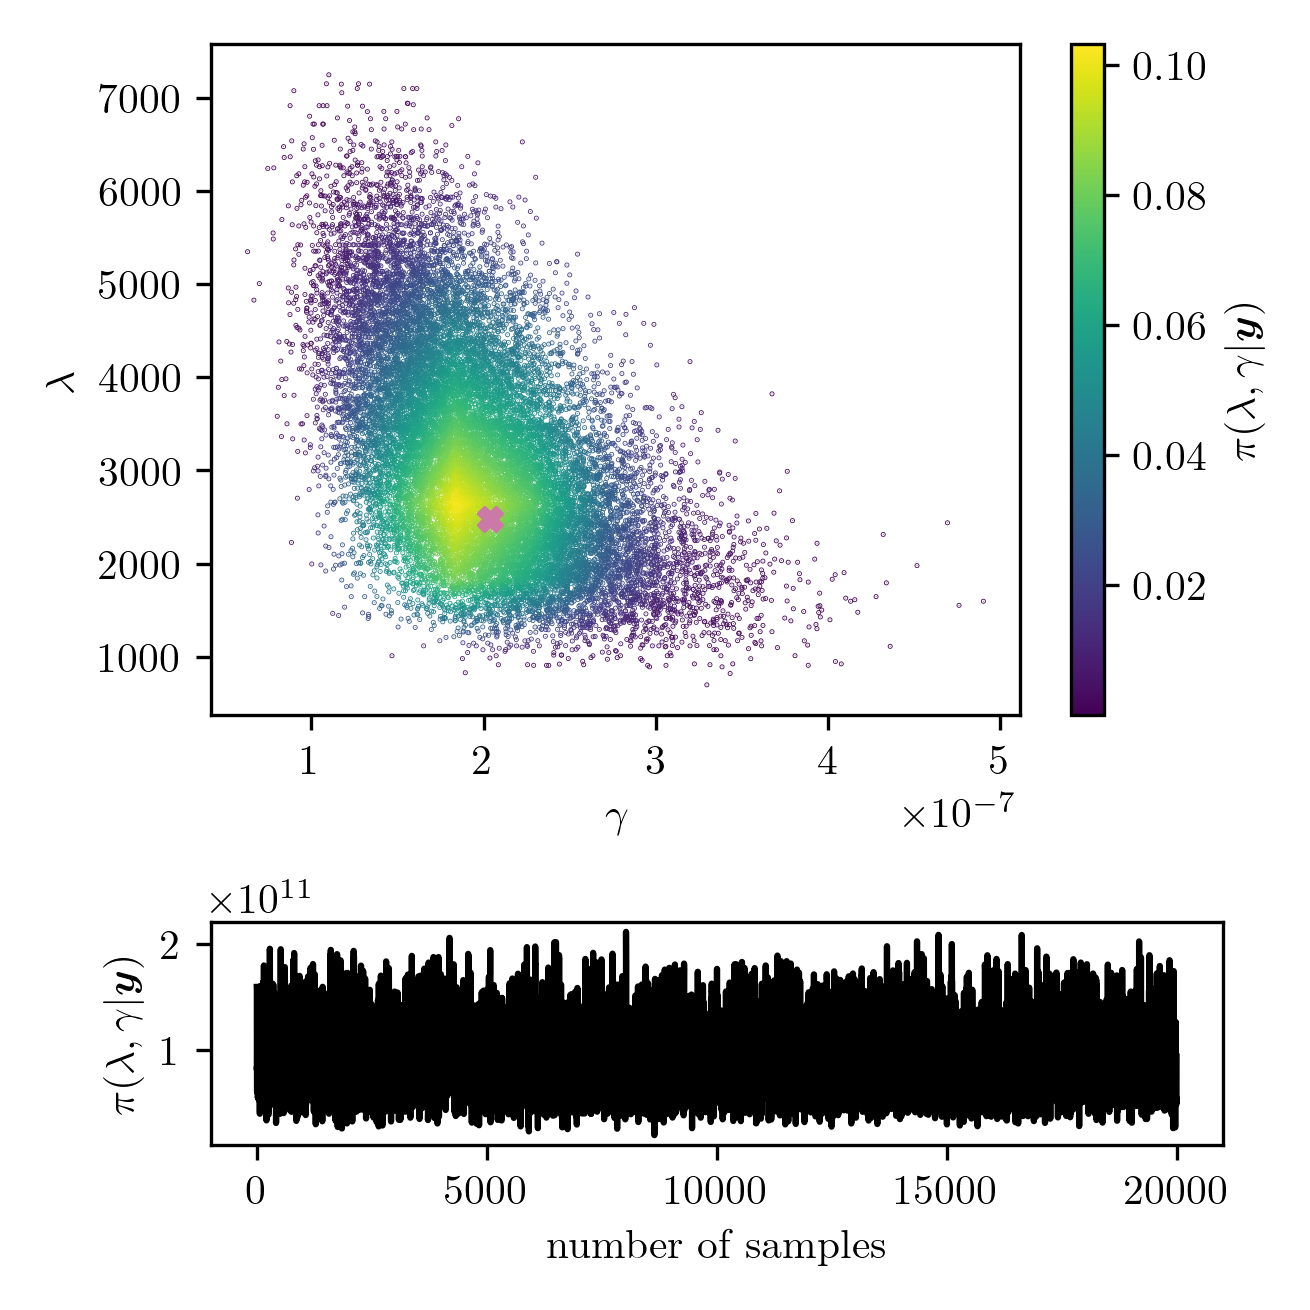
\includegraphics{ScatterplusHistoPlusTT.png}
	\caption[Scatter plot of samples from marginal posterior, including weighting from TT approximation; trace plot of the marginal posterior samples.]{We scatter plot the samples of $\lambda = \delta / \gamma $ and $\gamma$ from the marginal posterior $\pi(\lambda , \gamma  | \bm{y})$ and colour code the samples using the TT approximation of $\pi(\lambda , \gamma  | \bm{y})$. The mode of $(\lambda_0 , \gamma_0)$ of $\pi(\lambda , \gamma  | \bm{y})$ is marked by the pink cross. To show ergodicity we plot the trace of the samples of the MWG sampler below.}
	\label{fig:ScatterPlotTT}
\end{figure}
\clearpage

%\subsubsection{Sample from Marginal Posterior Distribution}
%\label{subsec:firstMarg}

%\begin{algorithm}[!ht]
%	\caption{Metropolis within Gibbs for $\pi(\lambda, \gamma | \bm{y})$}
%	\begin{algorithmic}[1]
%		\STATE Initialise  \( \bm{\theta}^{(0)}  =( \lambda^{(0)} , \gamma^{(0)}  ) \) and set burn-in $N_{\text{burn-in}}$
%		\FOR{ \( k = 1, \dots, N^{\prime} \)}
%		\STATE Propose \( \lambda \sim \mathcal{N}(\lambda^{(t-1)}, 0.8 \lambda_0)  \)
%		\STATE Compute
%		\[ \alpha( \lambda  | \lambda^{(t-1)}) = \min \left\{ 1, \frac{\pi(\lambda | \gamma^{(t-1)}, \bm{y})  }{\pi(\lambda^{(t-1)}| \gamma^{(t-1)}, \bm{y})}  \right\} \]
%		\STATE Draw $u \sim \mathcal{U}(0,1)$
%		\IF{$\alpha \geq u$ }
%		\STATE Accept and set \( \lambda^{(t)} = \lambda \)
%		\ELSE  
%		\STATE Reject and keep \(\lambda^{(t)} = \lambda^{(t-1)} \)
%		\ENDIF
%		\STATE Draw $\gamma^{(t)} | \lambda^{(t)} ,\bm{y} \sim \text{Gamma} \big( 0.5  \, m + 2, 0.5 \, f(\lambda^{(t)}) + 10^{-10}(1 + \lambda^{(t)}) \big) $
%		\ENDFOR
%		%\STATE Output: $ \bm{\theta}^{(N_{\text{burn-in}})}, \dots,  \bm{\theta}^{(k)} , \dots,   \bm{\theta}^{(N)} \sim \pi(\bm{\theta}| \bm{y}) $
%		\STATE Output: $ (\lambda, \gamma)^{(N_{\text{burn-in}})}, \dots,  (\lambda, \gamma)^{(k)} , \dots,   (\lambda, \gamma)^{(N)} \sim \pi(\lambda, \gamma| \bm{y}) $
%	\end{algorithmic}
%	\label{alg:margPost}
%\end{algorithm}

\subsubsection{Full Posterior Ozone Mean and Variance}
\label{subsec:firstCond}
Then we evaluate the normally distributed conditional posterior distribution
\begin{align}
	\bm{x}| \delta, \gamma, \bm{y}  \sim \mathcal{N}\big( \underbrace{ (\bm{A}^T \bm{A} + \delta / \gamma \bm{L} )^{-1} \bm{A}^T \bm{y}}_{\bm{x}_{\lambda}}, ( \underbrace{ \gamma \bm{A}^T \bm{A} + \delta \bm{L} }_{\gamma \bm{B}_{\lambda}}  )^{-1} \big) \, \label{eq:CondPost},
\end{align}
as in Eq. \ref{eq:CondPostLin}, with $\lambda = \delta / \gamma $
In this thesis, we compute the mean
\begin{align}
	\mu_{\bm{x}|\bm{y}} = \int \bm{x}_{\lambda} \pi(\lambda| \bm{y}) \text{d}\lambda \approx \sum \bm{x}_{\lambda_i} \pi(\lambda_i| \bm{y}) \, , \label{eq:MeanInt}
\end{align} and covariance
\begin{align}
	\Sigma_{\bm{x}|\bm{y}} = \int \gamma^{-1}  \pi(\gamma | \bm{y} ) \, \text{d} \gamma \, \int  \bm{B}_{\lambda}^{-1} \, \pi(\lambda | \bm{y} )  \, \text{d} \lambda  \approx \sum {\gamma_i}^{-1}\pi(\gamma_i| \bm{y}) \sum \bm{B}_{\lambda_i}^{-1}\pi(\lambda_i| \bm{y})\, \label{eq:CovInt}
\end{align}
of $\pi(\bm{x}| \delta, \gamma, \bm{y})$ as weighted expectations, by quadrature \cite[Sec. 2.1]{Dick_Kuo_Sloan_2013}, with $\sum \pi(\lambda_i| \bm{y}) = \sum \pi(\gamma_i| \bm{y}) = 1$.
The weights $\pi(\lambda_i| \bm{y})$ and $\pi(\gamma_i| \bm{y})$ are either given by the TT approximation or by the bins for the sample-based histograms.
If calculating the variance is too costly, the RTO method (see Sec. \ref{subsec:RTO}) may be a feasible alternative to draw a sample from Eq. \ref{eq:CondPost}.


Based on the marginal posterior distribution $\pi(\lambda, \gamma| \bm{y})$ we calculate the mean and covariance of the conditional posterior $\pi(\bm{x} |\lambda, \gamma, \bm{y})$ by quadrature as in Eq. \ref{eq:MeanInt} and Eq. \ref{eq:CovInt}.
We can either use the sample based histogram bins as weights or the TT approximation to integrate over marginal approximations $\pi(\lambda| \bm{y})$ and $\pi( \gamma | \bm{y})$.
More precisely, for the sample based evaluation, the height of the histogram bars act as quadrature weights, e.g. $\pi(\lambda_i| \bm{y})$ at the centre $\lambda_i$ of each bin.
Then, we obtain the full conditional mean $\bm{\mu}_{\bm{x}|\bm{y}}$ and covariance matrix $\bm{\Sigma}_{\bm{x}|\bm{y}}$ as weighted expectations.
Again, we use Cholesky decomposition to invert $\bm{B}_{\lambda} = \bm{A}^T \bm{A} + \lambda \bm{L}$ and to calculate $\bm{x}_{\lambda} = (\bm{A}^T \bm{A} + \lambda \bm{L} )^{-1} \bm{A}^T \bm{y}$.
In total we have to evaluate $\bm{x}_{\lambda}$ and invert $\bm{B}_{\lambda}$ 20 times to obtain mean and covariance of $\pi(\bm{x}|\bm{y})$, Fig. \ref{fig:O3Samp}, which takes less than $0.2$s.
We plot posterior samples of $\pi(\bm{x}|\bm{y})$ in Fig. \ref{fig:O3Samp}, where we set negative ozone VMR to zero.
The fact that we have to deal with negative ozone values is due to the poor prior choice of $\pi(\bm{x}|\delta)$.
Note, that the sample mean is slight larger than posterior mean at heights where the data is noise dominated, and the ozone values are determined by the prior, or where the ground truth is close to zero.
This indicates that we should use a different more physical based prior or model to parametrise the ozone profile.
Note, that the posterior samples do not represent the ozone peak at around $80$km.
\begin{figure}[ht!]
	\centering
	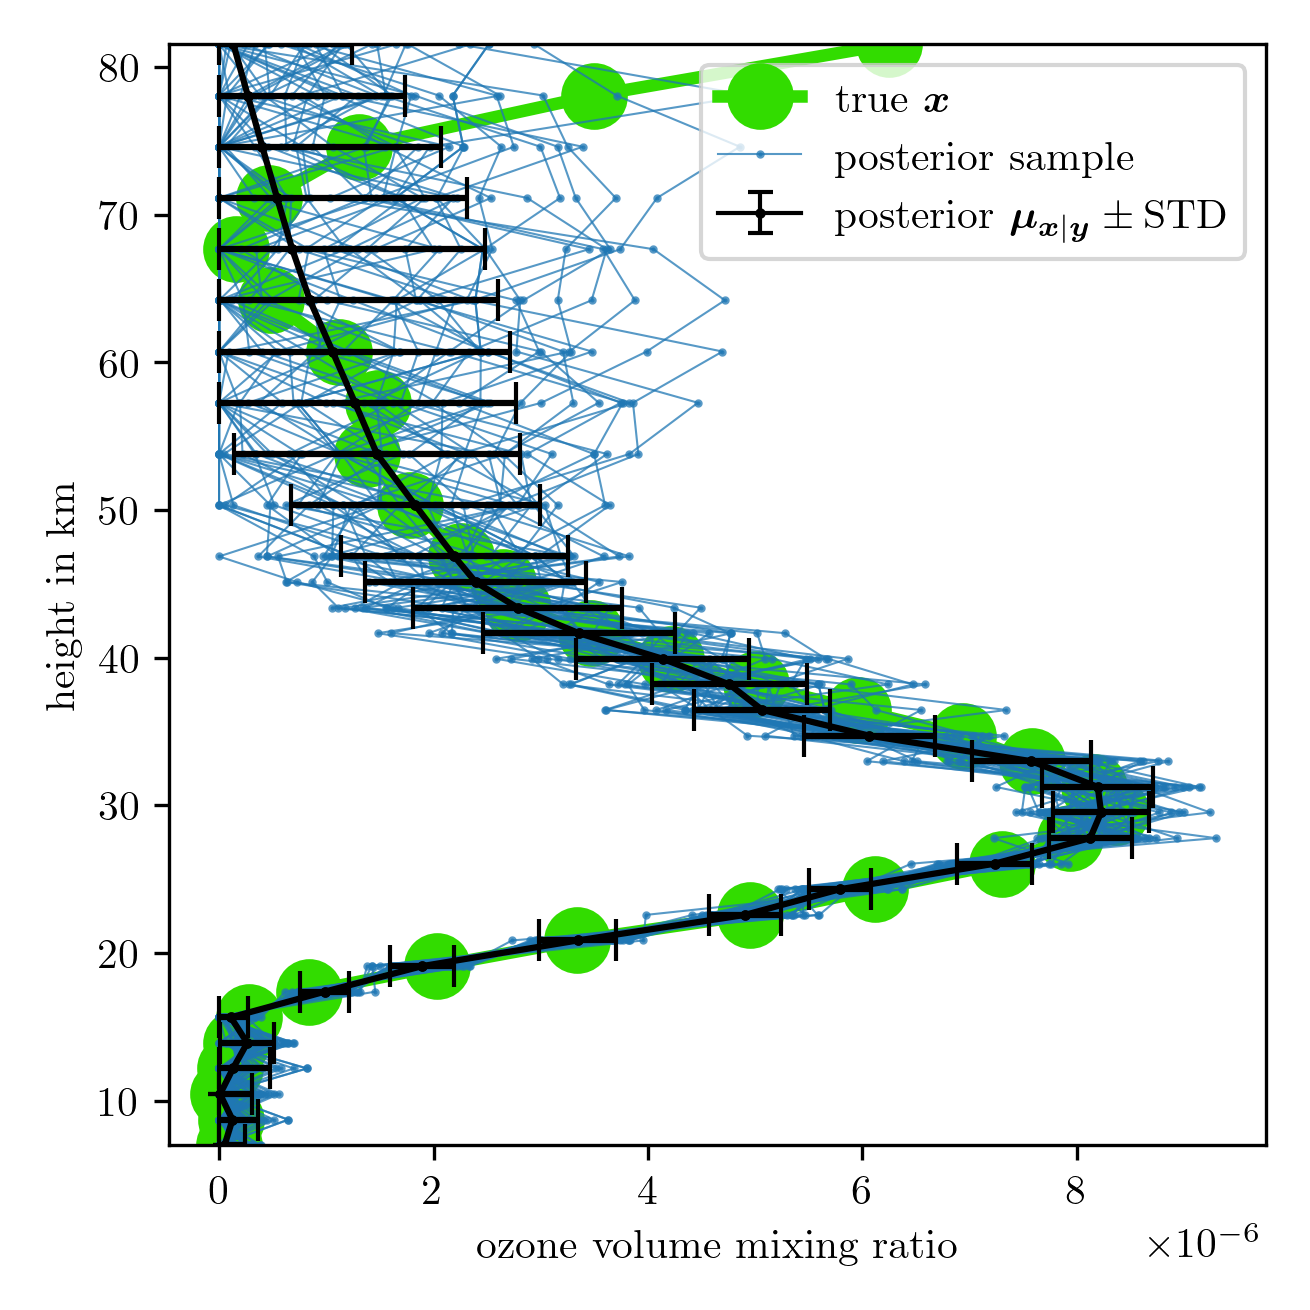
\includegraphics{FirstTestRes.png}
	\caption[Ozone samples of the full posterior.]{We draw ozone samples from the full posterior distribution $\pi(\bm{x}| \bm{y})$ after characterising mean and covariance of $\pi(\bm{x}| \bm{y})$ by weighted expectations over the marginal posterior $\pi(\lambda,\gamma | \bm{y})$. we determine  $\pi(\lambda, \gamma | \bm{y})$ either through sampling or via TT approximation based on the linear forward map $\bm{A}_L$. Note that we set negative values ozone VMR values to zero. We will use those samples to find the affine map $\bm{M}$, see section \ref{sec:affineMap}}
	\label{fig:O3Samp}
\end{figure}

\paragraph{Errors due to number of grid points}
we plot RMS for mean and variance compared to a solutop with 200 grid points.
The relative error behaves proportionally to $1/N$, see Fig. \ref{fig:MCError} and Eq. \ref{eq:MCerr}, and we consider a relative error less than $0.1\%$ good enough.
This happens roughly at a bin size of 25, which is our TT grid size.
Note that we exclude the error due to $\tau_{\text{int}}$ the IACT and that we choose the grid according to the sampled values so that the sampling region is the same as the region in which we approximate the posterior distributions.
.\begin{figure}[ht!]
	\centering
	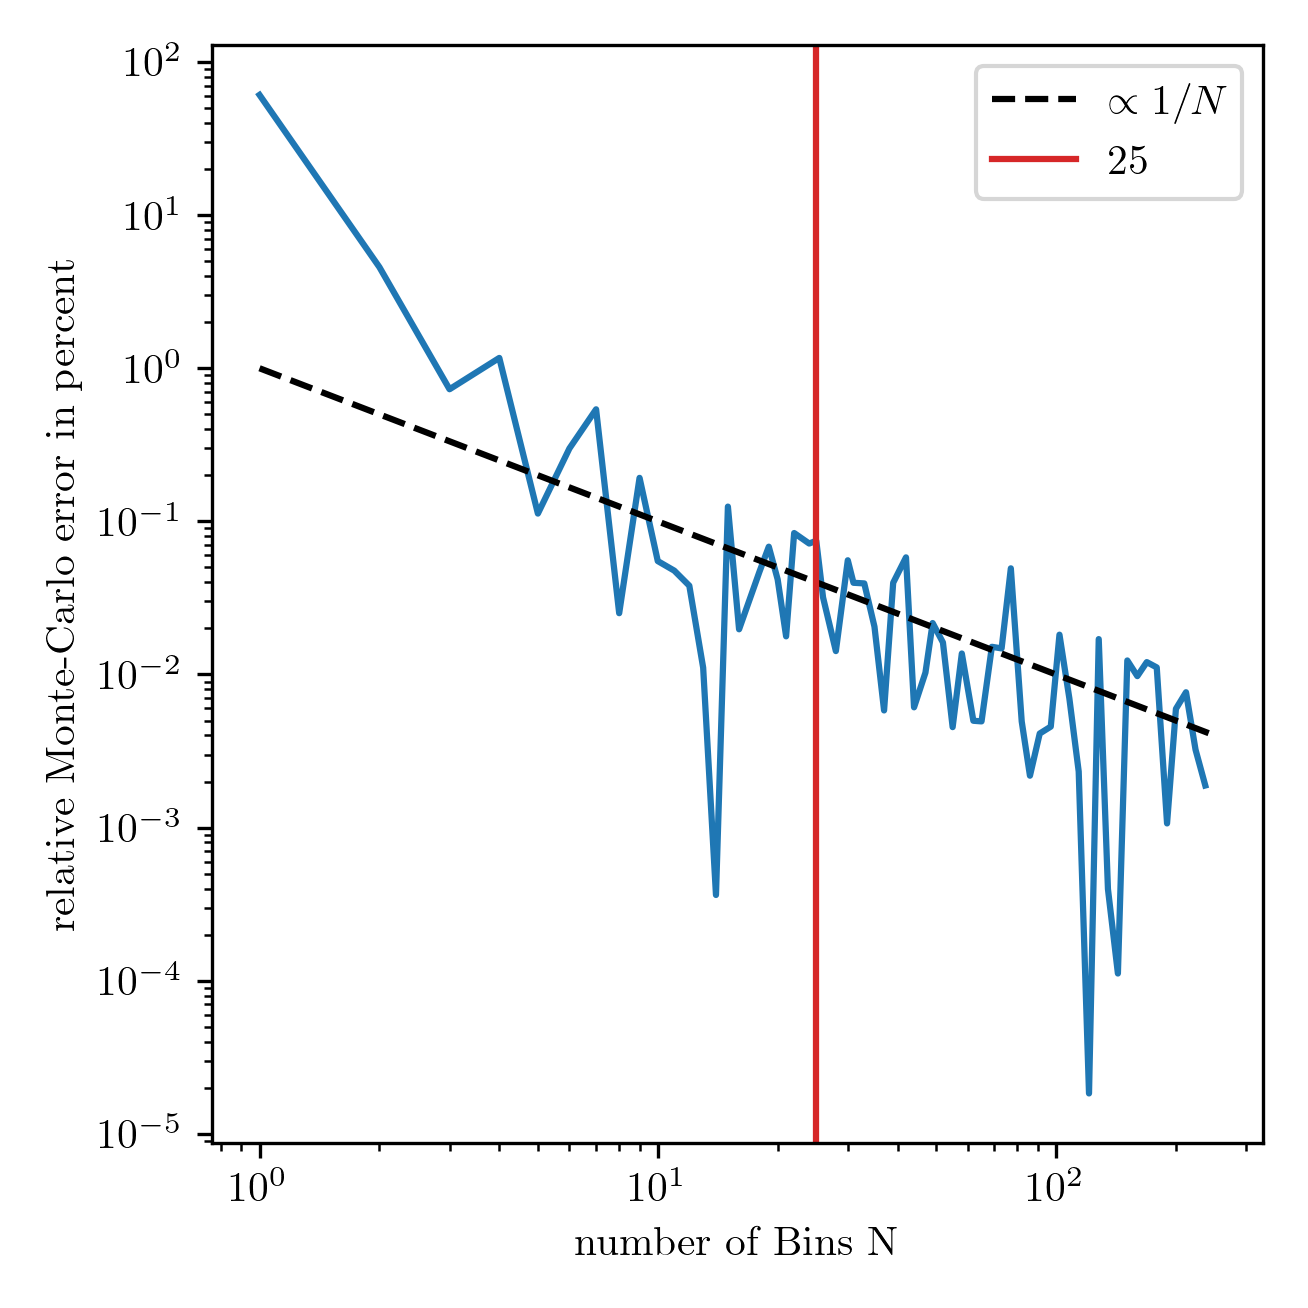
\includegraphics{MeanAssPT.png}
	\caption[Assessment of Monte-Carlo error.]{Assessment of Monte-Carlo error, where we calculate the relative error of the mean due to binning up the samples compared to the sample mean $||\bm{\mu}_{\text{samp}} -\bm{\mu}_{\text{distr}} ||/ || \bm{\mu}_{\text{samp}}||$.}
	\label{fig:MCError}
\end{figure}
%marginal Ozone Pressure Temperature
The error of is influeced by rank and gridsize
interploation error
\clearpage
%\subsubsection{Randomize then optimize -- RTO}
%For the RTO method we start by drawing an independent hyper-parameter sample $ ( \delta, \gamma) \sim \pi(\delta, \gamma | \bm{y})$ from the samples of the MwG.
%Then we generate two independent Gaussian random variables $\bm{v}_1 \sim \mathcal{N}(\bm{0},\gamma  \bm{A}^T_L \bm{A}_L)$ and $\bm{v}_2 \sim \mathcal{N}(\bm{0}, \delta \bm{L})$.
%Here  can use Cholesky factorisation of $\bm{L} =\bm{L}_C\bm{L}^T_C $ and the multiplication rule for normal distributions so that $\bm{v}_1 \sim \sqrt{\gamma} \bm{A}_L^T \mathcal{N}(0,\bm{I})$ and $\bm{v}_2 \sim \sqrt{\delta} \bm{L}_C \mathcal{N}(0,\bm{I})$.
%Then we solve
%\begin{align}
%	\label{eq:FirstRTO}
%	\left( \gamma \bm{A}_L^T  \bm{A}_L +\delta \bm{L} \right) \bm{x} = \gamma \bm{A}_L^T \bm{y} + \bm{v}_1 + \bm{v}_2 \, ,
%\end{align}
%using Cholesky back and forward substitution, for $\bm{x}$ and obtain one independent sample of $\pi(\bm{x}|\bm{y}, \bm{\theta})$.
%See Fig. \ref{fig:O3Samp}, where we plot $m = $ samples of the conditional posterior.
%
%The histogram in is binned as we intergate over it to 7 bins

\section{Approximate non-linear Forward Model with an Affine Map} 
\label{sec:affineMap}
Given the posterior distribution for ozone $ \pi(\bm{x}|\bm{y})$, we can now approximate the non-linear forward model 
\begin{align}
	\bm{A}_{NL} \approx \bm{M A}_L \, ,
\end{align}
with an affine map $\bm{M}$, see Fig. \ref{fig:affinStrat} for the summarised strategy.
Here we write $\bm{A}_{NL} \bm{x}$, which implies that we construct the non-linear forward model and compute non-linear noise-free data $\bm{A}(\bm{x},\bm{p},\bm{T})$ based on ground truth pressure and temperature.
\begin{figure}[htb!]
	\centering
	\begin{tikzpicture}
		\node[rectnode] at (0,0) (Oy)    {$\bm{y}$};
		\node[roundnode2] at (0,-2) (x)     {$\bm{x}$};
		\node[rectnode] at (-1.75,-4) (NLy)    {$\bm{V}$};%{$\bm{A}_{NL}\bm{x}$};
		\node[rectnode] at (1.75,-4) (y)    {$\bm{W}$};%{$\bm{A}_L\bm{x}$};
		\draw[->, very thick] (Oy.south) -- (x.north); 
		\draw[->, very thick] (x.south west) -- (NLy.north); 
		\draw[->, very thick] (x.south east) -- (y.north); 
		\draw[->, very thick] (NLy.east) -- (y.west); 
		\node[align=center] at (1,0) (l1) {Data};
		\node[align=center] at (3.5,-2) (f2) {Ozone Profiles from $\pi(\bm{x}|\bm{y}) $};
		\node[align=center] at (1.75,-1) (l1) {$\pi(\lambda , \gamma  | \bm{y})$ with $\bm{A}_L$};
		
		
		\node[align=center] at (-4.75,-4) (f3) {non-linear forward model};
		\node[align=center] at (4.25,-4) (f4) {linear forward model};
		\node[align=center] at (0,-5) (f5) {$\bm{A}_{NL} \approx \bm{M A}_L$ };
		
		\node[align=center] at (0,-4) (f5) {affine Map \\ $\bm{M}$};
		
	\end{tikzpicture}
	\caption[Strategy to find affine map.]{The strategy to find the affine map consist of evaluating the marginal posterior for ozone using the linear forward model. Then we draw ozone samples from the conditional posterior and calculate noise free data based on the linear and non-linear forward model. Next we find a mapping in between those two space so that we can approximate the non-linear forward model using an affine map and the linear forward model.}
	\label{fig:affinStrat}
\end{figure}
Using posterior ozone samples we generate two affine subspaces and then find the mapping between those.
The subspace $\bm{W}$ is created by noise free data based on the linear model $\bm{A}_L$ and $\bm{V}$ by noise free data based on the non-linear model $\bm{A}_{NL}$, given $m$ samples $\bm{x}^{(j)} \sim \pi(\bm{x}|\bm{y})$ for $j = 1, \dots,m$.
We report a relative RMS difference between $\bm{W}$ and $\bm{V}$ of about $1\%$, which we aim to reduce through the affine map $\bm{M}$.
More specifically, the affine subspace associated with the linear forward model is 
\begin{align}
	\bm{W} = \begin{bmatrix}
		\vert&   &  \vert & & \vert \\
		\bm{A}_{L} \bm{x}^{(1)} &  \cdots& \bm{A}_{L} \bm{x}^{(j)} &  \cdots & \bm{A}_{L} \bm{x}^{(m)} \\
		\vert&   &  \vert & & \vert 
	\end{bmatrix}
	\in \mathbb{R}^{m \times m}
\end{align} and with the non-linear forward model is 
\begin{align}
	\bm{V} = \begin{bmatrix}
		\vert&   &  \vert & & \vert \\
		\bm{A}_{NL}\bm{x}^{(1)} &  \cdots& \bm{A}_{NL}\bm{x}^{(j)} &  \cdots & \bm{A}_{NL} \bm{x}^{(m)}  \\
		\vert&   &  \vert & & \vert 
	\end{bmatrix} = 
	\begin{bmatrix}
		\begin{array}{ccc}
			\horzbar & v_{1} & \horzbar \\
			& \vdots    &          \\
			\horzbar & v_{j} & \horzbar \\
			& \vdots    &          \\
			\horzbar &v_{m} & \horzbar
		\end{array}
	\end{bmatrix}\in \mathbb{R}^{m \times m} \, .
\end{align}
Then the we calculate affine map 
\begin{align}
	\bm{V}\bm{W}^{-1} = \bm{M} =
	\begin{bmatrix}
		\begin{array}{ccc}
			\horzbar & r_{1} & \horzbar \\
			& \vdots    &          \\
			\horzbar & r_{j} & \horzbar \\
			& \vdots    &          \\
			\horzbar &r_{m} & \horzbar
		\end{array}
	\end{bmatrix}\, \in \mathbb{R}^{m \times m} .
\end{align}
by solving $v_j =r_j \bm{W}$ for each row $r_j$ in $\bm{M}$, where $j = 1, \dots, m$, using the Python function \texttt{numpy.linalg.solve}.
We can do that because every measurement in the data vector $\bm{y}$ is independent of each other, and then every row $v_j$ of $\bm{V} \in \mathbb{R}^{m \times m}$ is independent of each other as well.

We asses the affine map by calculating the relative RMS difference $\lVert \bm{M}\bm{W} - \bm{V}  \rVert_{L^2} / \lVert \bm{M}\bm{W} \rVert_{L^2} $ between the mapped linear noise free data and the non-linear noise free data, which is approximately $0.001\%$.
\begin{figure}[ht!]
	\centering
	%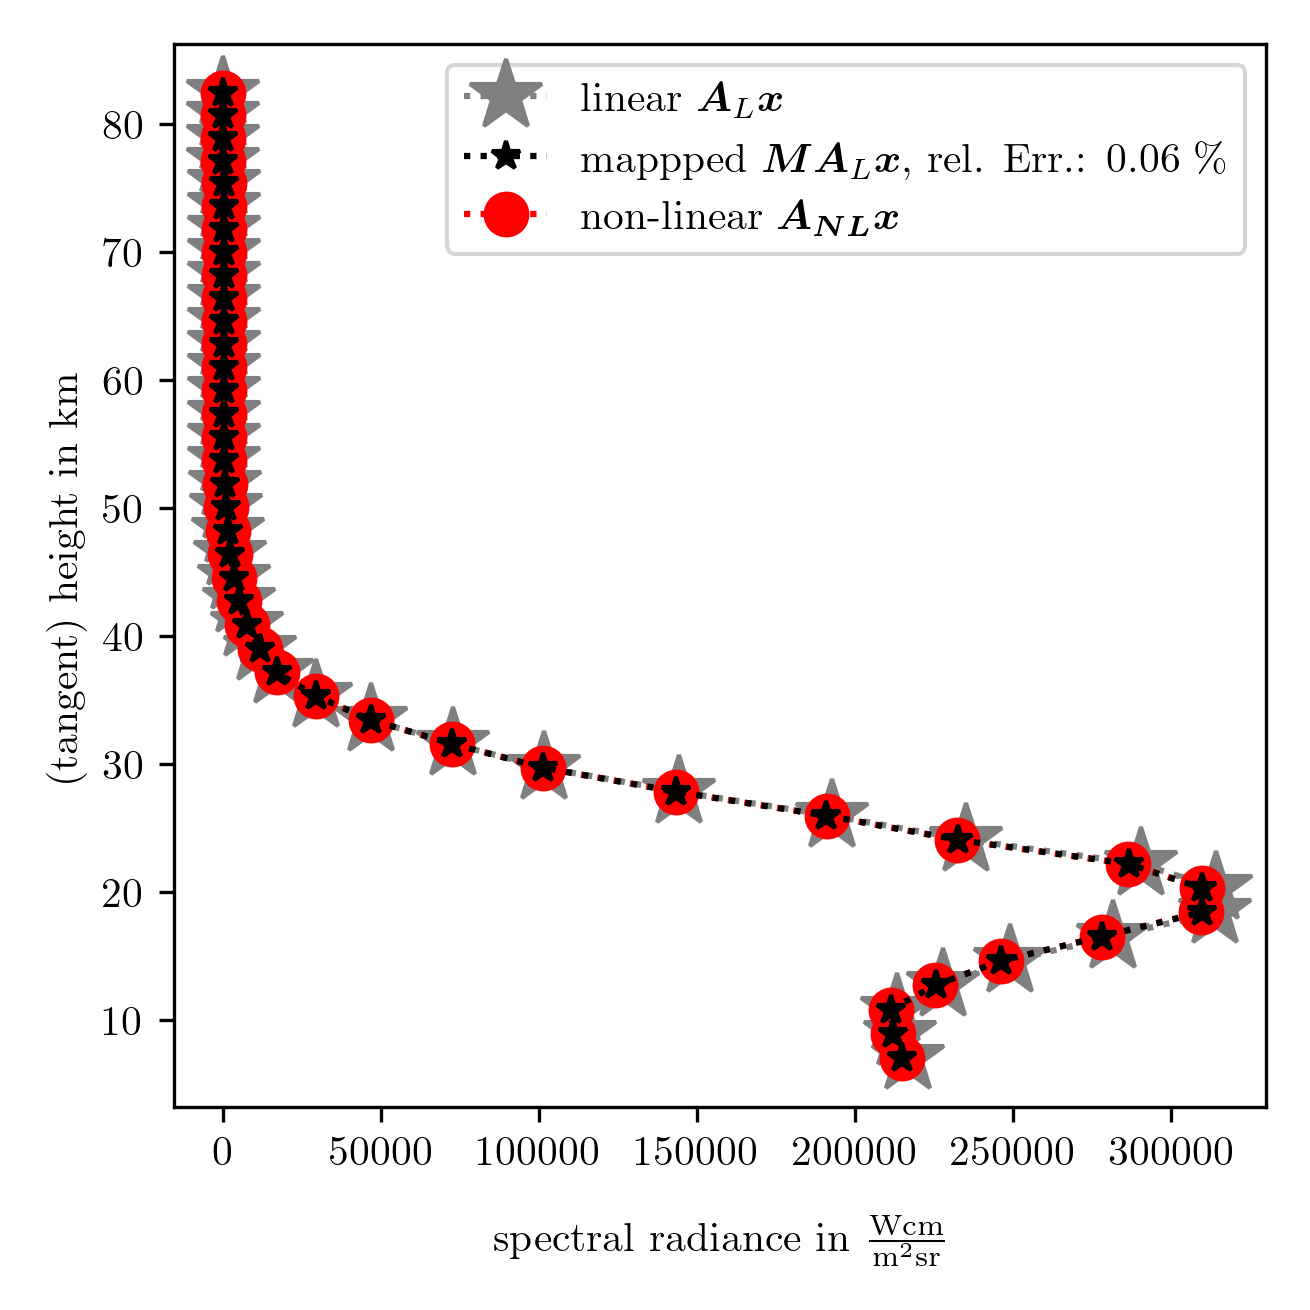
\includegraphics{SampMapAssesment.png}
	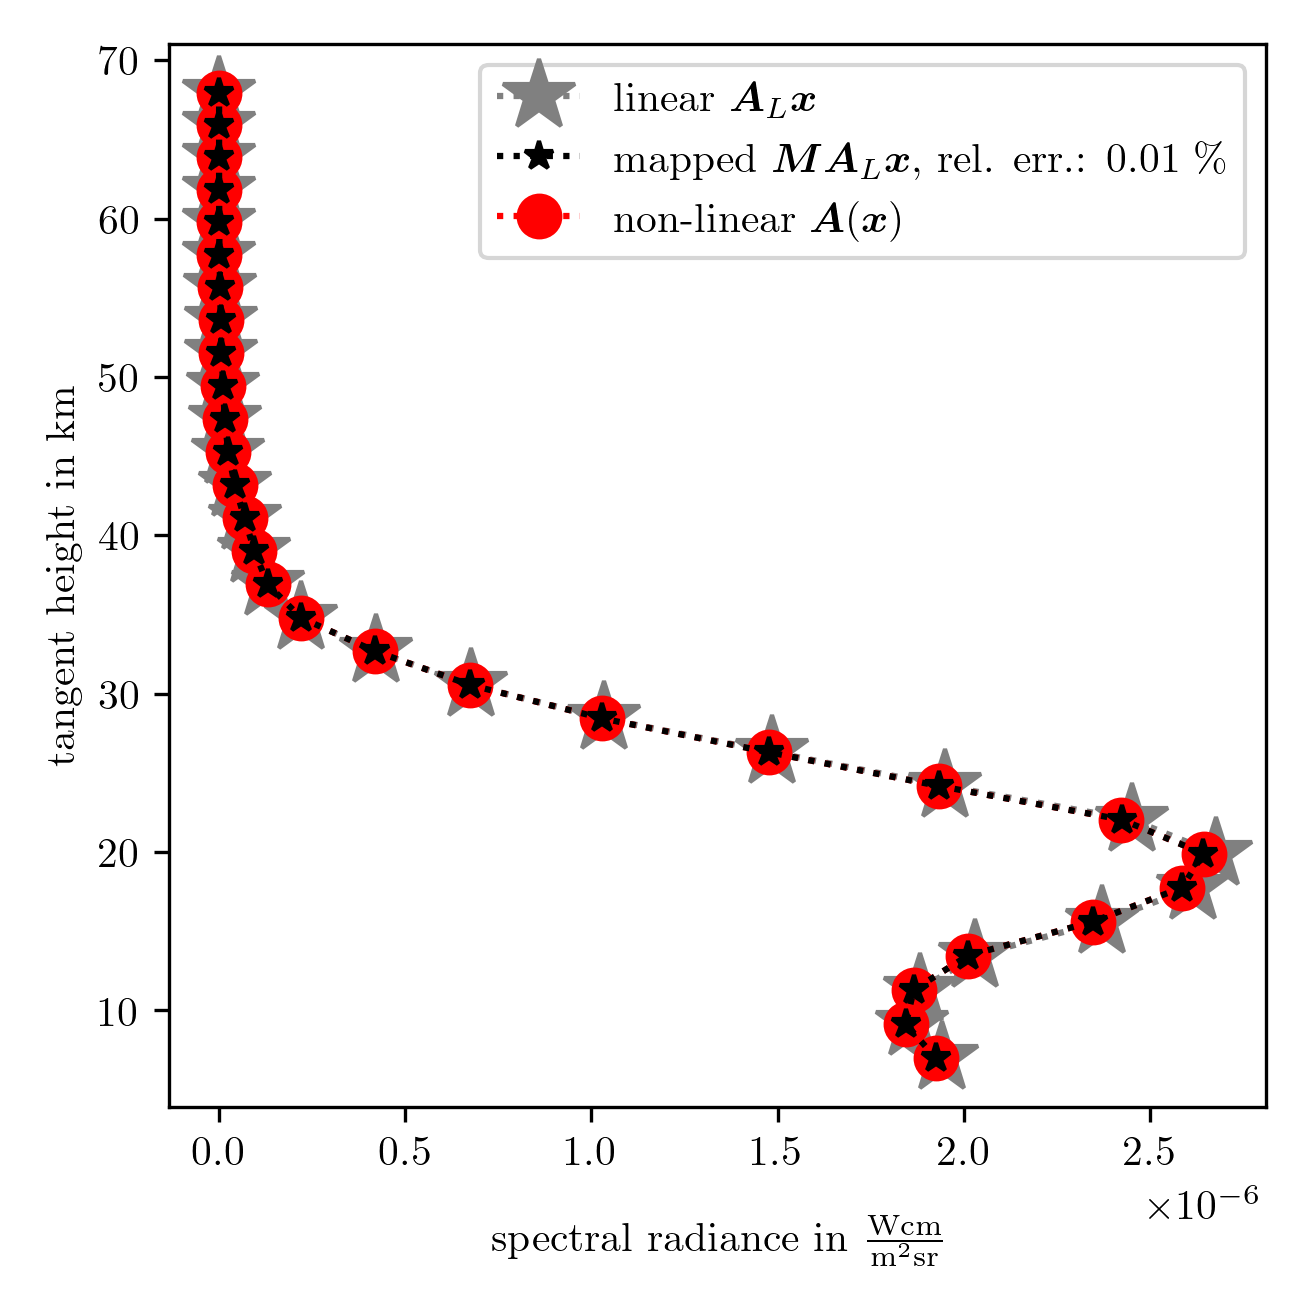
\includegraphics{SampMapAssesmentTT.png}
	\caption[Assessment of affine map.]{We asses how good we can map a new ozone sample $\bm{x} \sim \pi(\bm{x}|\bm{y})$ from the linear forward model onto the non-linear forward model using the previous calculated affine map $\bm{M}$. The sample has not been used to create this affine map. The gray stars represent noise free linear data, where as the red circles present noise free non-linear data. Then we map the linear noise free data onto the non-linear noise free data, black start, and provide the relative RMS error in between the mapped noise free data and the non-linear data.}
	\label{fig:MapAsses}
\end{figure}
In Fig. \ref{fig:MapAsses}, we show the mapping for one posterior ozone sample which has not been used to create this mapping.
In other word this is an unseen event not in the training data.
The relative RMS error for this approximation is roughly $0.03\%$ and much smaller than the relative difference between noise free linear data and non-linear data.
Consequently, from here onwards, we use the approximated forward map.

\clearpage
\section{Regularisation Solution vs. Bayesian Approach -- approximated Model}
\label{sec:ComparReg}%\section{Posterior Distribution of Ozone -- approximated Model}
With the affine approximation we define the forward model matrix
\begin{align}
	\bm{A}  \coloneqq \bm{M A}_L \,
\end{align}
using the affine map $\bm{M}$.
Here we compare the posterior distribution of ozone to a regularisation approach.

\subsection{Posterior Distribution for Ozone}
Again we us the MTC scheme and the exact same setup as in Sec. \ref{sec:FirstO3Post} to evaluate the marginal posterior and then the conditional posterior of ozone.

\subsubsection{Marginal Posterior}
The marginal posterior is defined as in Eq. \ref{eq:MargPostAppl}, but with updated forward model.
We initialise the MWG at the mode of $\pi(\lambda,\gamma| \bm{y})$ and approximate $f(\lambda)$ and $g(\lambda)$ around the mode as in Eq. \ref{eq:fAprox} and Eq. \ref{eq:gAprox}.
Then we run the MWG algorithm for $N = 10000$ plus $N_{\text{burn-in}} = 100$ steps and plot the samples in Fig. \ref{fig:MargPostHistTT} as well as the marginal approximations provided by the TT decomposition on the same grid as previously defined with same number of ranks (see Sec. \ref{subsec:FirstMTC}).
\begin{figure}[ht!]
	\centering
	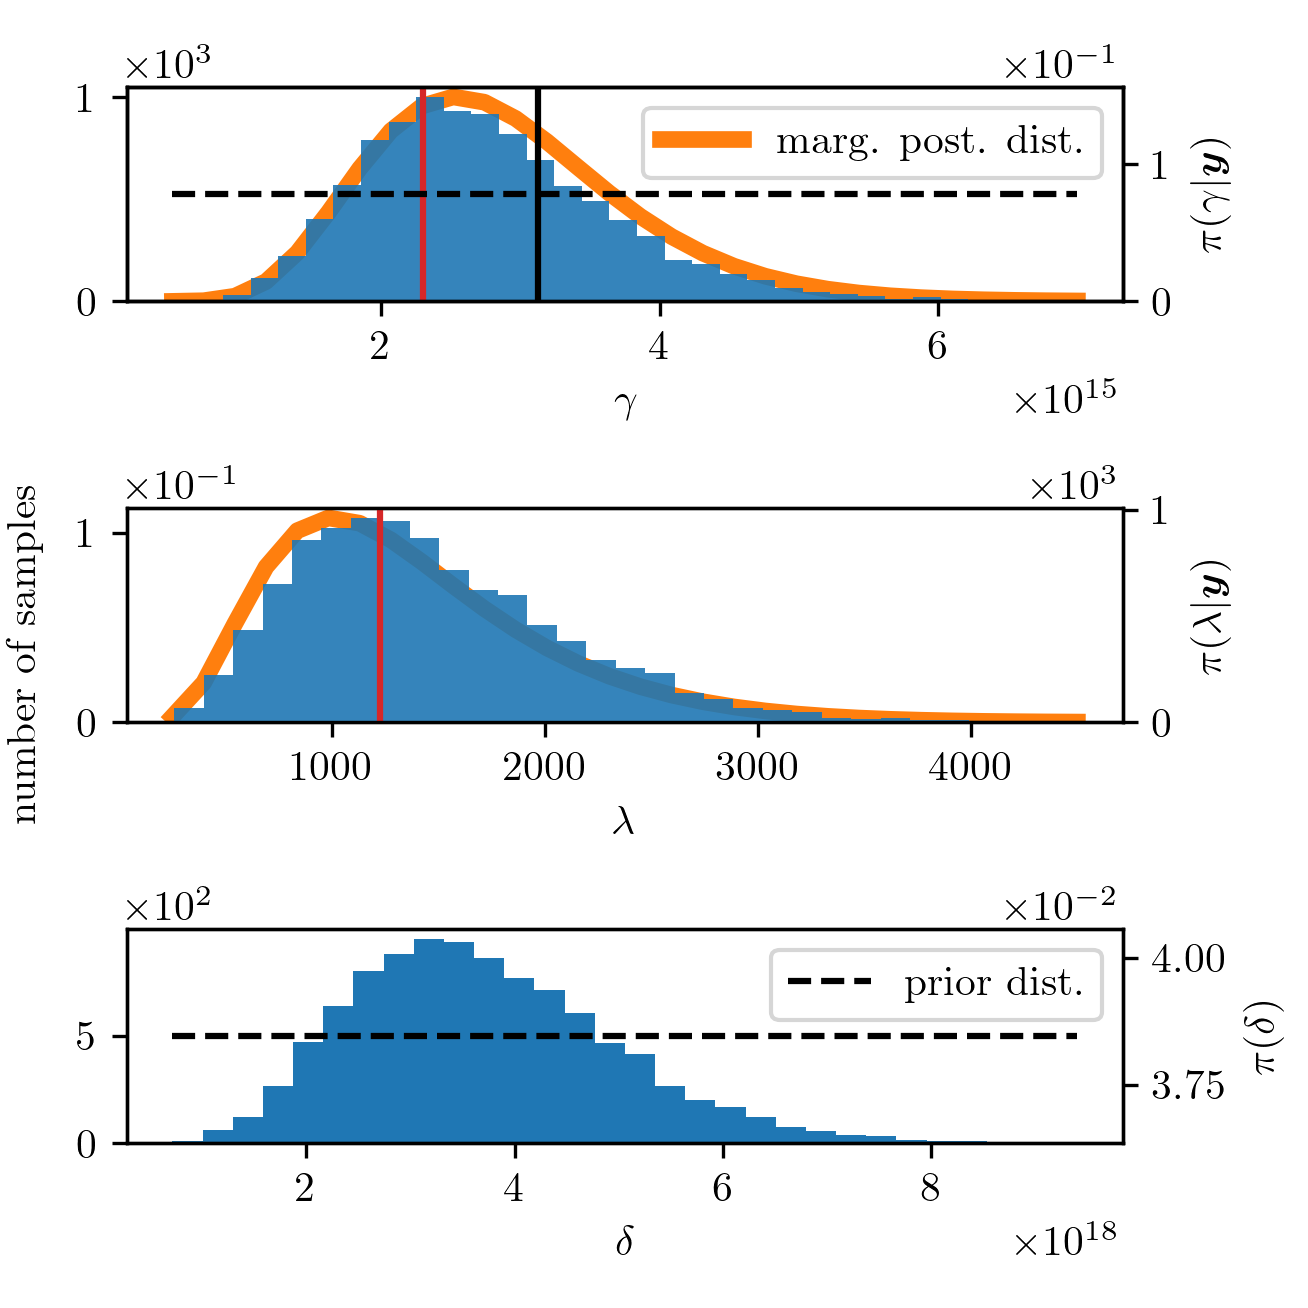
\includegraphics{secMargO3Res.png}
	\caption[Marginal posterior histograms and TT approximation as well as hyper-prior distribution.]{We plot the TT approximation of marginal posterior in orange and the samples as a histogram as well as the prior distribution with a dotted line. Note that we sample $\lambda$ and $\gamma$ using the Metropolis-within-Gibbs sampler and can calculate $\delta$ for every sample of the marginal posterior, we can not do this for the TT approximation. The regularised parameter corresponding to the regularised solution is marked thought the red vertical line at $\lambda_{\text{reg}} =$.}
	\label{fig:MargPostHistTT}
\end{figure}

\subsubsection{Full Posterior Ozone Mean and Variance}
Next, we characterise the conditional posterior $\pi(\bm{x}|\bm{y})$ as in Eq. \ref{eq:CondPost}. 
Again, we calculate the full posterior mean $\bm{\mu}_{\bm{x}|\bm{y}}$, see Eq. \ref{eq:MeanInt}, and covariance matrix $\bm{\Sigma}_{ \bm{x}|\bm{y}}$ \ref{eq:CovInt} as weighted expectation over a 20-point grid provided by either the marginal TT approximations of $\pi(\gamma| \bm{y})$ and $\pi(\lambda| \bm{y})$ or by the bins of the sample histogram as quadrature weights.
We plot the conditional mean and variance in Fig. \ref{fig:O3SolplsReg}, the regularised solution (see next section), and one sample from the posterior, which represents a feasible solution to this inverse problem.
We can see that the ground truth lays within 3 times of the STD (accounting for $\approx 99 \%$ of all posterior samples) around the mean except for the peak at around $80$km.
We also note that compared to the previously calculated mean and variance based on the linear forward model, see \ref{fig:O3Samp}, the approximated based posterior distribution does not differ significantly.
This is expected since the difference between the linear and non-linear forward map of $\approx 1 \%$ is small.
\begin{figure}[ht!]
	\centering
	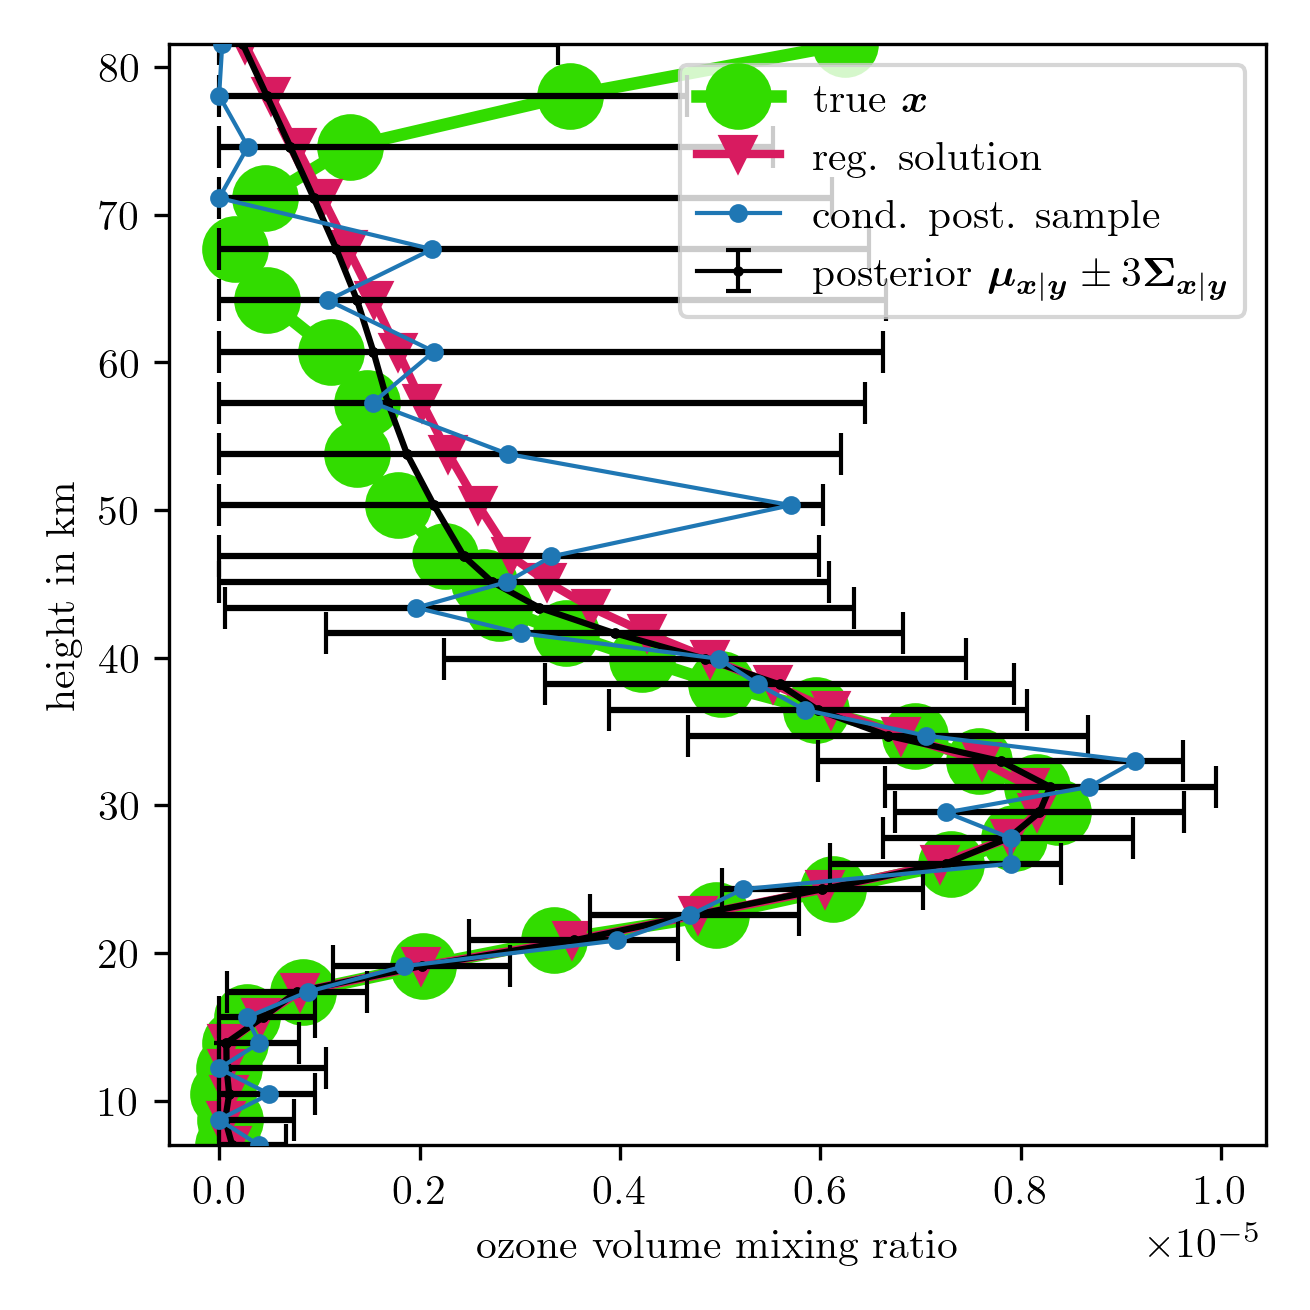
\includegraphics{SecRecResinclRegandSampl.png}
	%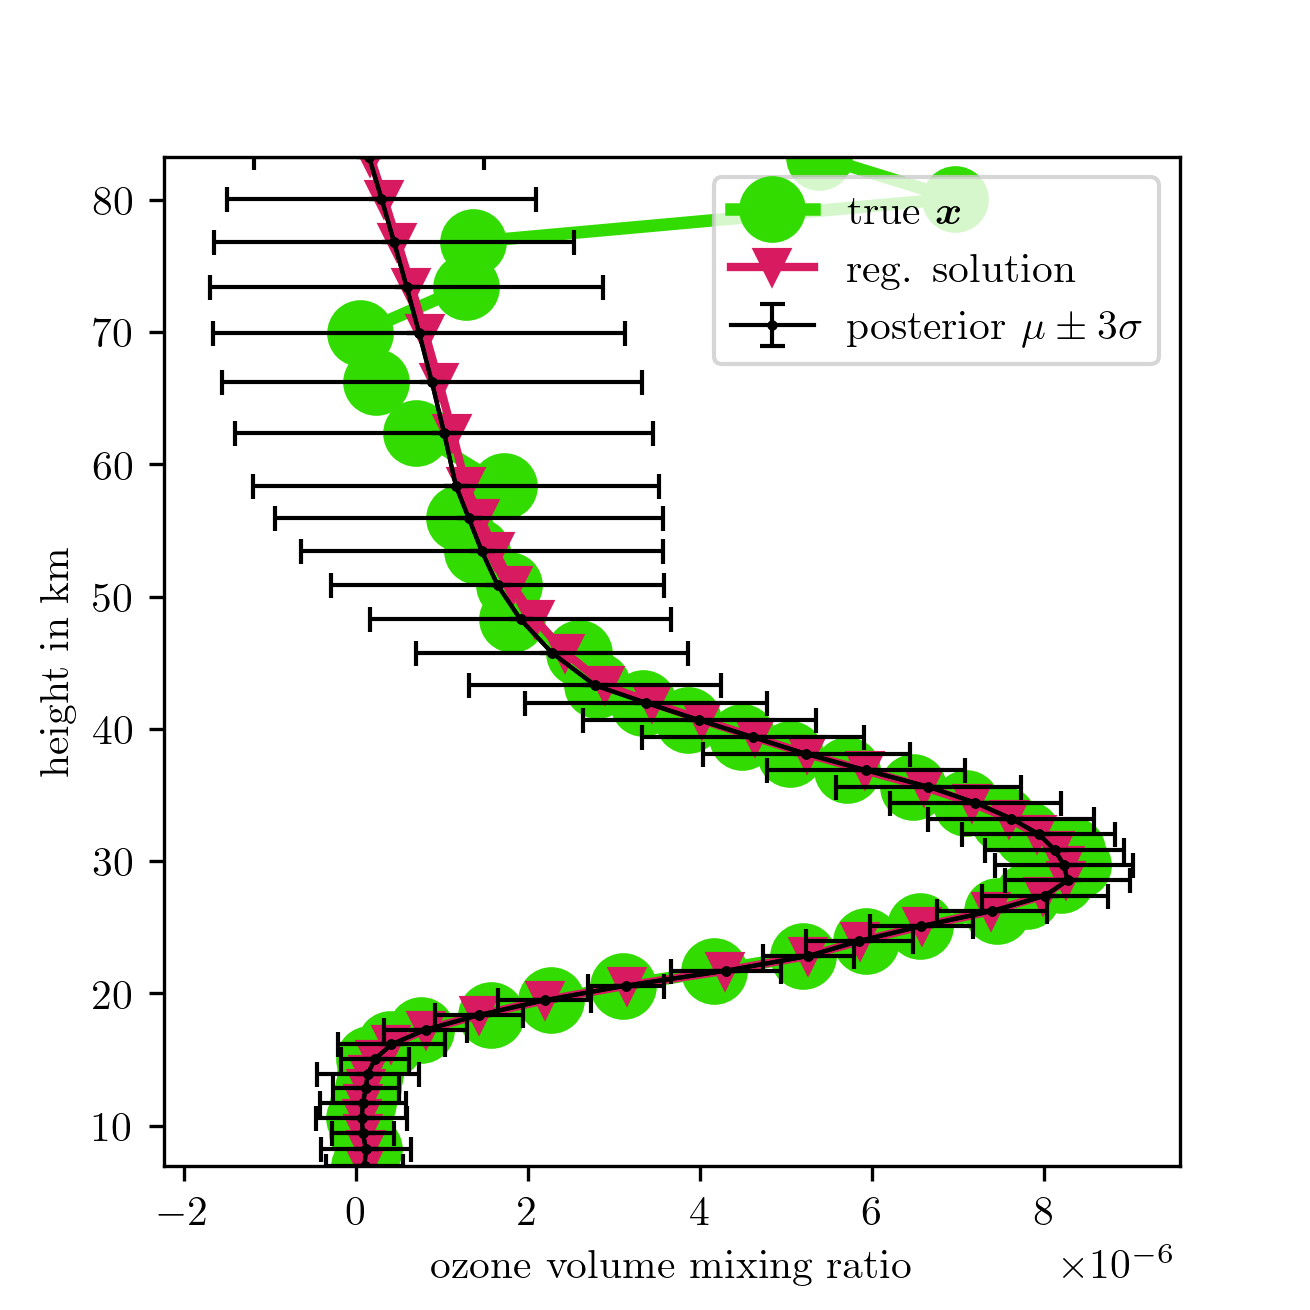
\includegraphics{SecRecResinclReg.png}
	\caption[Ozone posterior mean and variance and the regularised solution compared to the ground truth.]{We plot the conditional posterior mean and variance in black and the regularised solution on top of the ground truth ozone profile in green. We use the updated forward map $\bm{M}\bm{A}_L$}
	\label{fig:O3SolplsReg}
\end{figure}

Additionally in Fig. \ref{fig:PostCov}, we plot the singular values of the covariance matrix $\bm{\Sigma}_{ \bm{x}|\bm{y}}$, to visualise how many ozone values are informative.
We observe that the last 10 singular values are very small and correspond to ozone values at the high altitudes $\gtrsim 45$km with a large variance, see Fig. \ref{fig:O3SolplsReg}.
This is also roughly the region where we introduce a higher correlation structure due (see Eq. \ref{eq:GLapl} Sec. \ref{subsec:PriorModelO3}) and the samples are determined by the prior.
\begin{figure}[ht!]
	\centering
	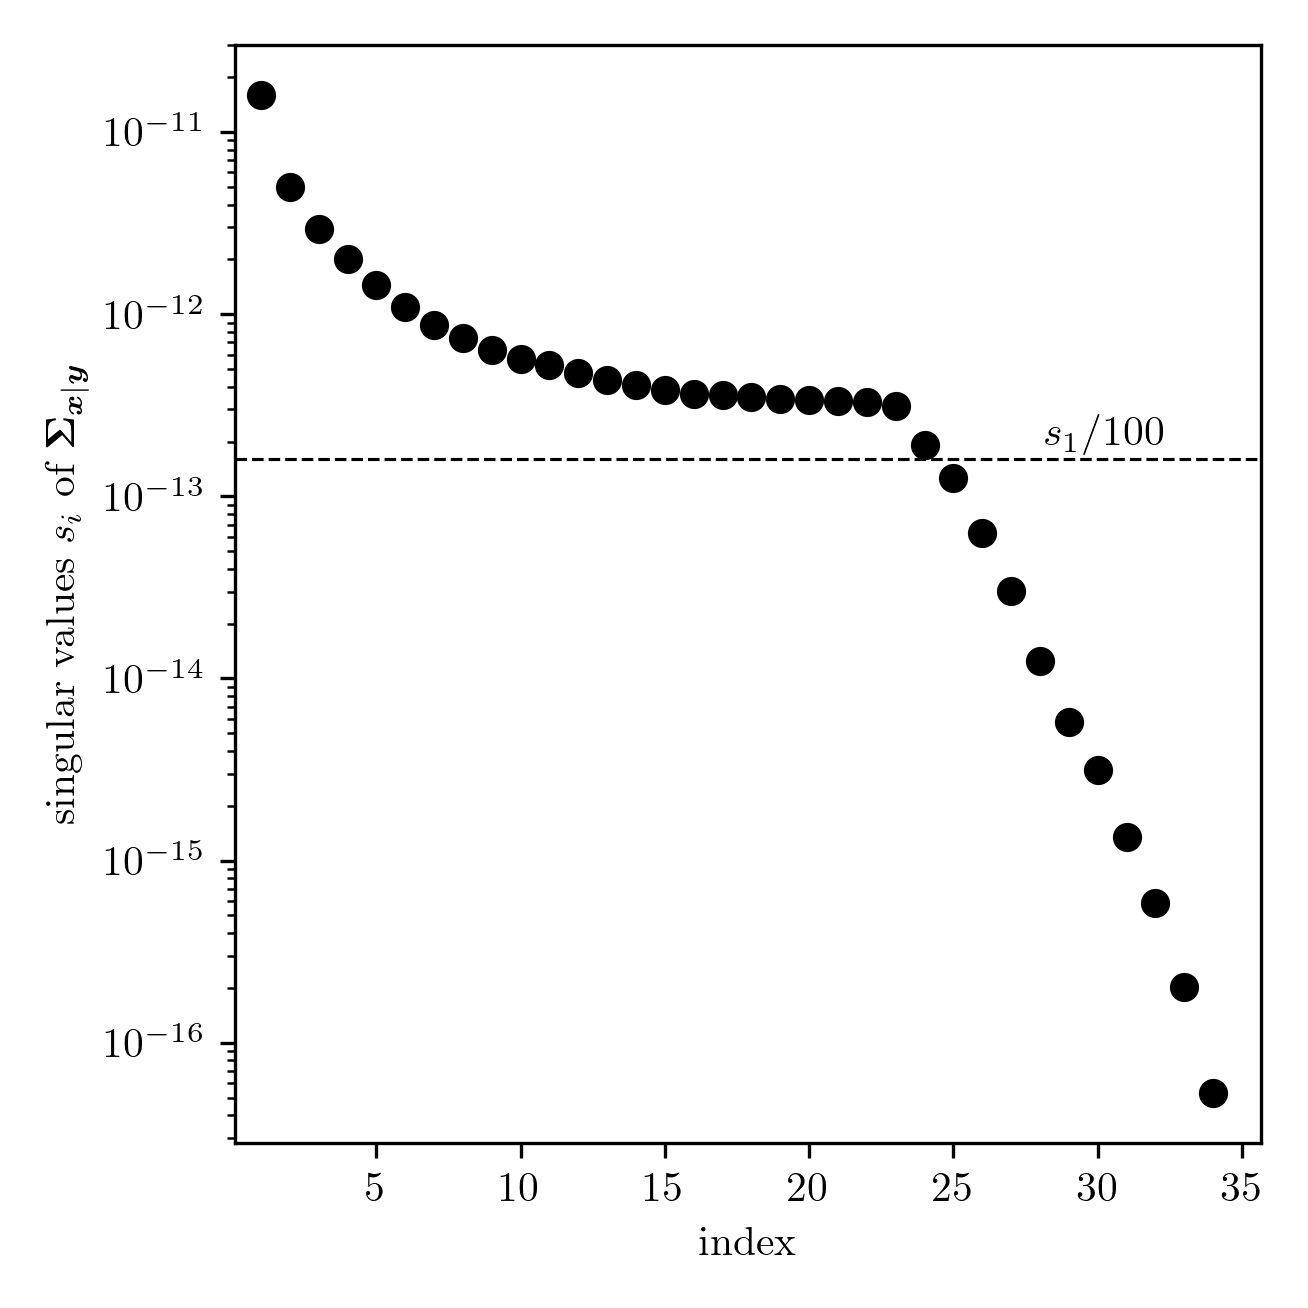
\includegraphics{CovSing.png}
	\caption[Singular values of the posterior covariance matrix]{Singular values of the covariance matrix of $\bm{\Sigma}^{-1}_{ \bm{x}|\bm{y}} = (\sum (\bm{A}^T \bm{A} + \bm{L})^{-1})^{-1}$ of the posterior distribution $\pi(\bm{x}|\bm{y})$ for ozone.}
	\label{fig:PostCov}
\end{figure}
\clearpage


\subsection{Solution by Regularisation}
\label{sec:reg}
Since we claim that Bayesian analysis is superior to regularisation methods we compare the MTC method to a Tikhonov regularisation solution, see Sec. \ref{sec:regularise} and \cite{fox2016fast}.
This is most similar to our chosen linear-Gaussian Bayesian framework.
The Tikhonov regularised solution is defined as in~\cite{hansen2010discrete, fox2016fast} 
\begin{align}
	\bm{x}_{\lambda} =\underset{ \bm{x}}{\arg \min}\,  \lVert \bm{A}\bm{x} - \bm{y} \rVert_2^2 + \lambda \bm{x}^T \bm{L} \bm{x} \, ,
	\label{eq:XLam}
\end{align}
with the regularisation parameter $\lambda$.
The regularised solution is typically calculated by solving the normal equations, see Sec. \ref{sec:regularise},
\begin{align}
	\bm{x}_{\lambda} = (\bm{A}^T\bm{A} + \lambda \bm{L} )^{-1} \bm{A}^T \bm{y} \label{eq:xLam} \, .
\end{align}
To find the best regularised solution, we use the L-curve method~\cite{hansen1993use}.
Within this method we compute $\bm{x}_\lambda$, for 200 different $\lambda$ values in between $10^{0.5}$ to $10^{6.5}$ and plot the solution semi norm $\sqrt{\bm{x}_\lambda^T\mathbf{L} \bm{x}_\lambda}$ against the data misfit norm $\lVert \bm{A}\bm{x}_\lambda - \bm{x} \rVert$, see Figure \ref{fig:LCurve}. 
The best regularised solution corresponding to the corner of the L-curve is located at the point of maximum curvature, see triangle in Fig. \ref{fig:LCurve}, which we find with the kneedle algorithm~\cite{satopaa2011kneedle} using the python function \texttt{kneed.KneeLocator} in less $0.1$s.
\begin{figure}[ht!]
	\centering
	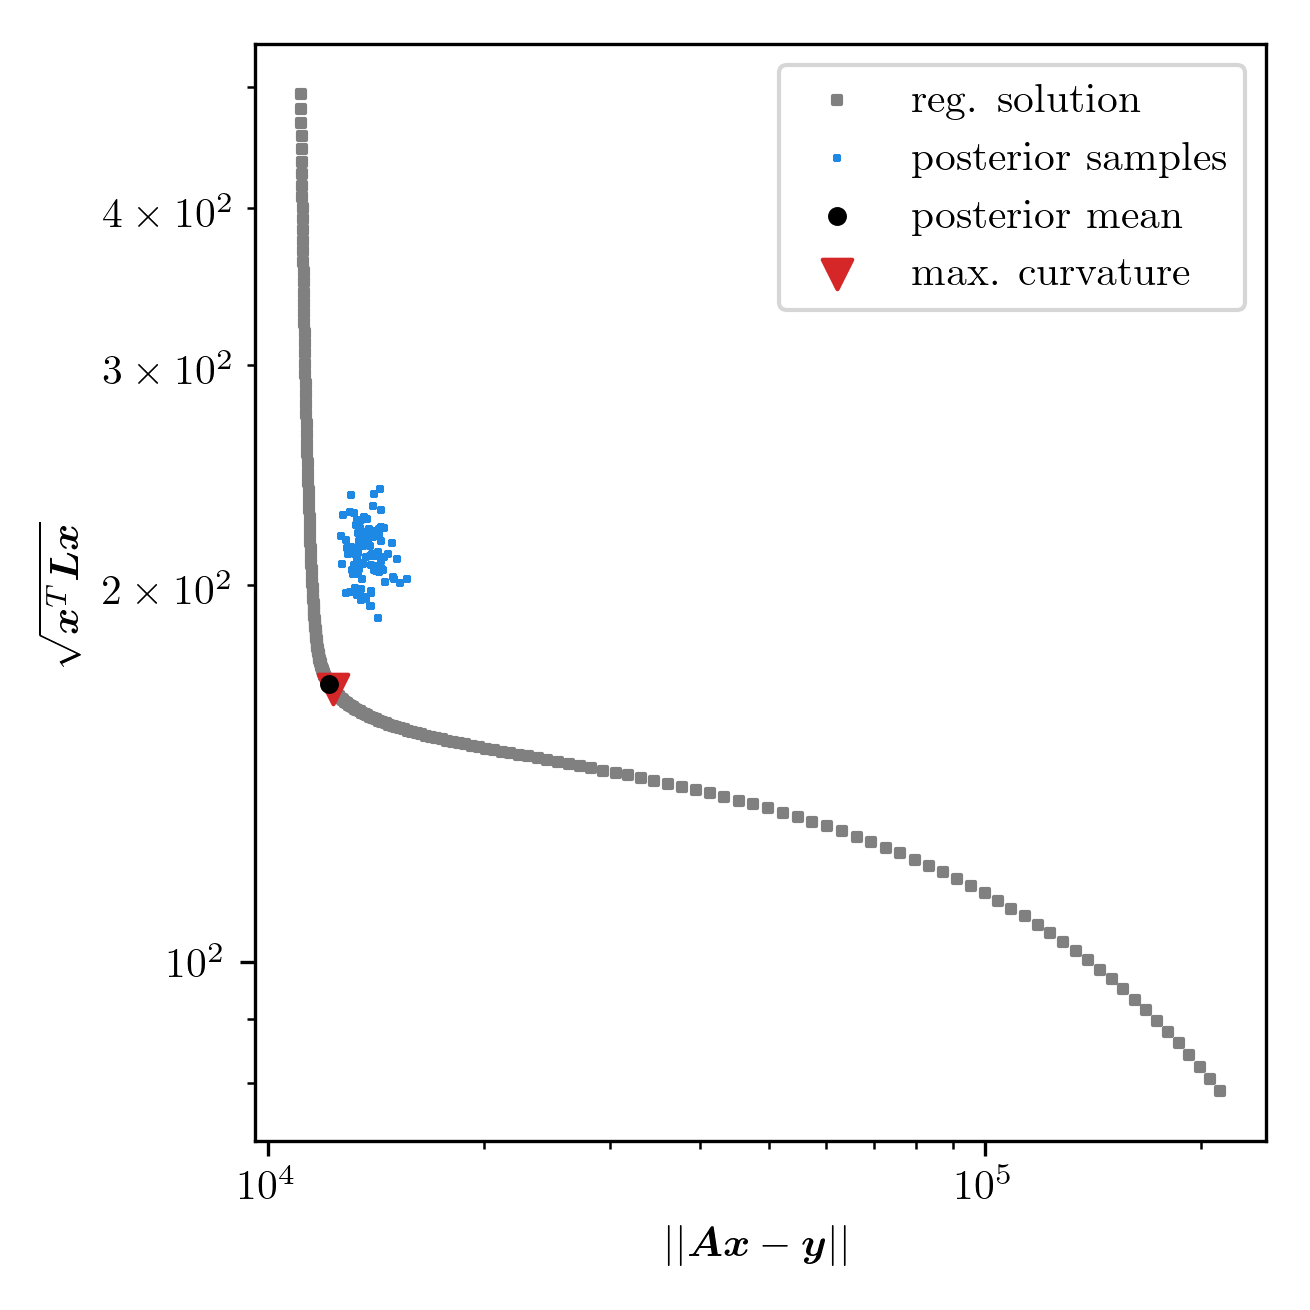
\includegraphics{LCurvePhD.png}
	\caption[Plot of the L-curve to find the regularised solution.]{We calculate regularised solution as in Eq. \ref{eq:} and plot the regularised semi norm $\sqrt{\bm{x}^T\bm{Lx}}$ against the data misfit norm $||\bm{Ax} -\bm{y} ||$ to find the regularised solution at the point of maximum curvature of the so-called L-Curve. Additionally we calculate the data misfit norm and the regularised norm for the ozone posterior and for samples of the conditional posterior distribution. \textcolor{red}{make box around Kneedle reagion}}
	\label{fig:LCurve}
\end{figure}

We plot the regularised solution in Fig. \ref{fig:O3SolplsReg} and observe that it is very similar to the posterior mean.
It is pretty clear that the regularised solution accounts for only one possible solution and does not provide uncertainties. The regularised solution is not similar to the samples drawn from the posterior $\pi(\bm{x}| \bm{y})$, see also Fig. \ref{fig:O3Samp}.
In Fig. \ref{fig:LCurve}, the samples of $\pi(\bm{x}| \bm{y})$ lie above the L-Curve where as the posterior mean and the regularised solution lie on the L-Curve.
This does make sense, if one thinks about the mean (average over non-smooth samples) and the regularised solution as extremely smooth ozone profiles, see also Sec. \ref{sec:regularise}.
In contrast the samples are less regularised and hence lie above the L-Curve, but have a similar data misfit norm and as already mentioned are all feasible solution to the data.
Neither the regularisation solution nor the posterior ozone profiles capture the ozone peak of the ground truth at high altitudes.
\clearpage

\section{Hierarchical Bayesian Framework for Ozone, Pressure and Temperature}
\label{sec:FullBay}
\begin{figure}[thb!]
	\centering
	\begin{tikzpicture}
		\node[roundnode2] at (-4.5,6.5) (Q)     {$\bm{Q}$};
		\node[roundnode2] at (-3,5) (x)     {$\bm{x}$};
		\node[align=center] at (-1,4) (A)    {$\bm{A} \coloneqq  \bm{M}\bm{A}_L$};
		\node[roundnode2] at (-1,2.5) (u)    {$\Omega$};
		\node[rectnode] at (-1,1) (y)    {$\bm{y}$};
		\node[roundnode2] at (-2.5,2.5) (e)    {$\bm{\eta}$};
		\node[roundnode2] at (-6.25,6.5) (S)    {$\bm{\Sigma}$};
		\node[roundnode2] at (-7.75,8) (s)    {$\gamma$};
		\node[roundnode2] at (-6,8) (d)    {$\delta$};
		\node[roundnode2] at (3,6.5) (t)     {$\bm{T}$};
		\node[roundnode2] at (-1,6.5) (p)     {$\bm{p}$};
		\node[roundnode2] at (1,5) (pt)     {$\bm{p}/\bm{T}$};
		\node[roundnode2] at (0,8) (b1)    {$b$};
		%\node[roundnode2] at (1,8) (b2)    {$b_2$};
		%\node[roundnode2] at (-2,8) (h1)    {$h_{0}$};
		\node[roundnode2] at (-1.5,8) (p0)    {$p_0$};
		\node[roundnode2] at (2.25,8) (ht)    {$\bm{h_T}$};
		\node[roundnode2] at (3.25,8) (ct)    {$T_0$};
		\node[roundnode2] at (4.25,8) (at)    {$\bm{a}$};
		
		\node[roundnode2] at (0,10) (b1hyp)    {$\bm{\theta}_{b}$};
		%\node[roundnode2] at (-2.5,10) (h1hyp)    {$\bm{\theta}_{h_{0}}$};
		\node[roundnode2] at (-1.5,10) (p0hyp)    {$\bm{\theta}_{p_{0}}$};
		\node[roundnode2] at (2,10) (hthyp)    {$\bm{\theta}_{\bm{h}_T}$};
		\node[roundnode2] at (3.25,10) (cthyp)    {$\bm{\theta}_{T_{0}}$};
		\node[roundnode2] at (4.5,10) (athyp)    {$\bm{\theta}_{\bm{a}}$};
		
		\node[roundnode2] at (-7.75,10) (shyp)    {$\bm{\theta}_{\gamma}$};
		\node[roundnode2] at (-6,10) (dhyp)    {$\bm{\theta}_{\delta}$};
		
		%Lines
		
		
		\draw[->, very thick] (S) -- (e);
		\draw[->, mydotted, very thick] (s) -- (S);
		\draw[->, very thick] (u) -- (y);
		\draw[->, mydotted, very thick] (A) -- (u);
		\draw[->, mydotted,  very thick] (x) -- (A.north west);
		\draw[->, mydotted, very thick] (p) -- (pt);
		\draw[->, mydotted, very thick] (t) -- (pt);
		\draw[->, mydotted, very thick] (pt) -- (A.north east);
		%\draw[->, mydotted, very thick] (h1) -- (p);
		\draw[->, mydotted, very thick] (p0) -- (p);
		\draw[->, mydotted, very thick] (b1) -- (p); 
		%\draw[->, very thick] (b2.south) -- (p.east); 
		\draw[->, mydotted, very thick] (d) -- (Q); 
		\draw[->, mydotted, very thick] (e) -- (y); 
		
		\draw[->, very thick] (Q.south east) -- (x.north west); 
		\draw[->, mydotted, very thick] (ht.south) -- (t.north west);
		\draw[->, mydotted, very thick] (ct.south) -- (t.north);
		\draw[->, mydotted, very thick] (at.south) -- (t.north east);
		
		
		\draw[->, very thick] (b1hyp) -- (b1);
		%\draw[->, very thick] (h1hyp) -- (h1);
		\draw[->, very thick] (p0hyp) -- (p0);
		\draw[->, very thick] (hthyp) -- (ht);
		\draw[->, very thick] (cthyp) -- (ct);
		\draw[->, very thick] (athyp) -- (at);
		\draw[->, very thick] (shyp) -- (s);
		\draw[->, very thick] (dhyp) -- (d);
		
		\node[fit=(s)(at),draw,dotted,black, rounded corners] {};
		\node[align =center] at (-3.75,8) (T1) {hyper-parameters};
		
	\end{tikzpicture} 
	\caption[Directed acyclic graph of Bayesian model for ozone, pressure and temperature.]{DAG of Bayesian model for ozone, pressure and temperature. The hyper-parameters $\bm{h}_T= \{ h_{T,1}, h_{T,2},h_{T,3},h_{T,4},h_{T,5},h_{T,6}\}$, $\bm{a} = \{ a_0, a_1, a_2,a_3,a_4,a_5,a_6\}$, $T_0$, $b$ and $p_0$ deterministically (dotted line) describe pressure parameter $\bm{p}$ through the function in Eq. \ref{eq:pressFunc}, and temperature parameter $\bm{T}$ through the function in Eq. \ref{eq:tempFunc}.
	In this case, we decide the hyper-prior distribution $\pi(\bm{h}_T,\bm{a},b, p_0)$ to be a normal distribution, determined by $\bm{\theta}_{\bm{h}_T},\bm{\theta}_{\bm{a}}, \bm{\theta}_{T_{0}},\bm{\theta}_{b} , \bm{\theta}_{p_0}$, which represent mean and variances. 
	The ozone parameter $\bm{x}$ is statistically (solid line) described by the prior distribution $\bm{x}| \delta \sim \mathcal{N}(0,\delta \bm{L}) $. 
	Here the hyper-parameter $\delta$ accounts for smoothness in the ozone profile and defines the precision matrix $\bm{Q} = \delta \bm{L}$, where $\bm{L}$ is graph Laplacian as in Eq. \ref{eq:GLapl}.
	The noise covariance $\bm{\Sigma} = \gamma^{-1} \bm{I}$ of the random noise vector $\bm{\eta} \sim \mathcal{N}(0,\gamma^{-1} \bm{I} ) $ is defined by the noise hyper-parameter $\gamma$.
	As in Sec. \ref{sec:BayModelO3} described, $\bm{\theta}_{\delta}$ and $\bm{\theta}_{\gamma}$ define the hyper-priors $\pi(\delta, \gamma)$.
	Then, we randomly observe a data set $\bm{y}$ from the space of all measurables $\Omega$ through the approximated froward model $\bm{M}\bm{A}_L$ including some added noise.
	Given the data we like to determine the posterior distribution over the hyper-parameters $\pi(\bm{h}_T,\bm{a},b, p_0, \delta, \gamma | \bm{y})$ first and then $\pi(\bm{x}|\bm{h}_T,\bm{a},b, p_0, \delta, \gamma, \bm{y})$ utilising the MTC scheme.}
	\label{fig:DAGComplete}
\end{figure}

As in Sec. \ref{sec:BayModelO3}, we use the DAG in Fig. \ref{fig:DAGComplete} to visualise the measurement process and correlations in between parameters.
We already see that the parameters pressure $\bm{p}$, temperature $\bm{T}$ and ozone $\bm{x}$ are correlated, and progress deterministically (dashed line) into the forward model, via $\bm{x} \times \bm{p} / \bm{T}$.
Through their respective prior distributions they generate a space of all possible noise free data $\Omega$, from which we observe some data included some added normally distributed noise $\bm{\eta}$.
This hierarchical Bayesian framework includes the hyper-parameters $p_0, b, \bm{h}_T, \bm{T}_0, \bm{a}$, for pressure and temperature, $\delta$ for ozone smoothness and $\gamma$ for noise precision.
Here pressure $\bm{p}$ and temperature $\bm{T}$ are functionally dependent on $p_0, b, \bm{h}_T, \bm{T}_0, \bm{a}$, see Eq. \ref{eq:tempFunc} and Eq. \ref{eq:pressFunc}.
Each of those hyper-parameters is described by the hyper-prior distribution $\pi(\gamma, \delta, p_0, b, \bm{h}_T, \bm{T}_0, \bm{a})$ defined by us.
Here $\bm{\theta}_{\gamma}, \bm{\theta}_{\delta},\bm{\theta}_{p_0},\bm{\theta}_{b},\bm{\theta}_{\bm{h}},\bm{\theta}_{T_0},\bm{\theta}_{\bm{a}}$ determine gamma distributions $\gamma, \delta \sim \pi(\bm{\theta}_{\gamma}, \bm{\theta}_{\delta})$, so that e.g. $\gamma \sim \Gamma(\alpha_{\gamma},\beta_{\gamma}) $ with $\bm{\theta}_{\gamma} = \{\alpha_{\gamma},\beta_{\gamma} \}$, and a normal distribution $p_0, b, \bm{h}_T, \bm{T}_0, \bm{a} \sim \pi( \bm{\theta}_{p_0},\bm{\theta}_{b},\bm{\theta}_{\bm{h}},\bm{\theta}_{T_0},\bm{\theta}_{\bm{a}})$, so that e.g. $b \sim \mathcal{N}(\mu_b, \sigma_b)$ and $\bm{\theta}_{b} = \{\mu_b, \sigma_b\}$.
We denote the forward model as $\bm{A} \coloneqq \bm{M} \bm{A}_L$.

\begin{table}
	\centering
	\begin{tabular}{ |c||c|c|c|c|c|   }
		\hline
		& &\multicolumn{2}{|c|}{TT bounds}& &\\
		\hline
		model parameters& priors&\makecell{lower}& \makecell{upper\\
		}&$\tau_{\text{int}}$&Context\\
		\hhline{|=||=|=|=|=|=|}
		$\gamma$ & $\mathcal{T}(1,10^{-10})$ &$5 \, 10^{-8}$ &$4.5 \, 10^{-7}$&  $ 9\pm 0.1$ &$\bm{y}$\\ \hline
		$\delta$ &$\mathcal{T}(1,10^{-10})$ & -&-& $1.5 \pm 0.1$ & $\bm{x}$\\ \hline
		$\lambda  = \delta / \gamma$ &- & 500&$10^4$& $3.5 \pm 0.3$ &$\bm{x}$\\ \hline
		$\bm{x}$ &$\mathcal{N}(0,\delta \bm{L})$ & -&-&-& $\bm{x}$\\ \hhline{|=||=|=|=|=|=|}
		$p_0$ &  $\mathcal{N}(1243,5)$&1229 &1259&$550 \pm 9$&$\bm{p/T}$\\ \hline
		$T_{0}$ &  $\mathcal{N}(288.15,4.5)$& 275 &302&$2446 \pm 76$&$\bm{p/T}$\\ \hline
		$h_{T,1}$ &  $\mathcal{N}(11,0.5)$&9.5 &12.5&$1820 \pm 49$ &$\bm{p/T}$\\ \hline
		$b$ &  $\mathcal{N}(0.167,5\,10^{-4})$& 0.165& 0.171 &$2813 \pm 92$&$\bm{p/T}$\\ \hline
		$h_{T,3}$ &  $\mathcal{N}(32.3,2.5)$&25.2&39.8&$394 \pm 5$&$\bm{p/T}$\\ \hline
		$a_{0}$ &  $\mathcal{N}(-6.5,0.01)$&-6.53 &-6.47&$330 \pm 4$&$\bm{p/T}$\\ \hline
		$h_{T,2}$ &  $\mathcal{N}(20.1,1.6)$&17.7 &22.3&$454 \pm 7$&$\bm{p/T}$\\ \hline
		$a_{1}$ &  $\mathcal{N}(0,0.1)$&-0.3 &0.3&$508 \pm 8$&$\bm{p/T}$\\ \hline
		$a_{2}$ &  $\mathcal{N}(1,0.01)$&0.97 &1.03&$341 \pm 5$&$\bm{p/T}$\\ \hline
		$a_{3}$ &  $\mathcal{N}(2.8,0.1)$&2.5 &3.1&$316 \pm 4$&$\bm{p/T}$\\ \hline
		$h_{T,4}$ &  $\mathcal{N}(47.4,5)$&45.9 &48.9&$324 \pm 4$&$\bm{p/T}$\\ \hline
		$a_{4}$ &  $\mathcal{N}(0,0.1)$&-0.3 &0.3&$335 \pm 4$&$\bm{p/T}$\\ \hline
		$h_{T,5}$ &  $\mathcal{N}(51.4,5)$&49.9 &52.9&$319 \pm 4$&$\bm{p/T}$\\ \hline
		$a_{5}$ &  $\mathcal{N}(-2.8,0.1)$&-3.1 &-2.5&$335 \pm 4$&$\bm{p/T}$\\ \hline
		$h_{T,6}$ &  $\mathcal{N}(71.8,3)$&62.5 &80.8&$347 \pm 5$&$\bm{p/T}$\\ \hline
		$a_{6}$ & $\mathcal{N}(-2,0.01)$ &-2.03 &-1.97&$320 \pm 4$&$\bm{p/T}$\\
		\hline
	\end{tabular}
	\caption[Summary of relevant parameter characteristics, bounds and sampling statistics.]{Summary of relevant parameter characteristics, bounds and sampling statistics. We denote $\mathcal{N}(\mu,\sigma)$ as the Gaussian and $\mathcal{T}(\alpha = \text{scale}, \beta = \text{rate})$ as the gamma distribution. The IACT $\tau_{\text{int}}$ is estimated as in \cite{UwerrM} from posterior samples based on the approximated forward map.}
	\label{tab:priors}
\end{table}

Then, we set up the hierarchical Bayesian framework
\begin{subequations}
	\begin{align}
		\bm{y} |  \bm{x},p_0,b,\bm{h}_{\bm{T}},T_0,\bm{a},\delta,\gamma  &\sim \mathcal{N}(\bm{A}(p_0,b,\bm{h}_{\bm{T}},T_0,\bm{a}) \, \bm{x}, \gamma^{-1} \bm{I}) \label{eq:likelihoodFull} \\
		\bm{x}| \delta  &\sim \mathcal{N}(\bm{0}, (\delta \bm{L})^{-1} ) \label{eq:priorXFull} \\
		\delta  &\sim \Gamma(\alpha_{\delta} , \beta_{\delta} )\label{eq:priorDelFull} \\
		\gamma  &\sim \Gamma(\alpha_{\gamma}, \beta_{\gamma})\label{eq:priorGamFull} \\
		\bm{a}  &\sim \mathcal{N}(\bm{\mu}_{\bm{a}}, \bm{\Sigma}_{\bm{a}})\\
		\bm{h}_{\bm{T}}  &\sim \mathcal{N}(\bm{\mu}_{T}, \bm{\Sigma}_{\bm{h}_T}) \\
		T_0  &\sim \mathcal{N}(\mu_{T_0}, \sigma_{T_0} )\\
		p_0  &\sim \mathcal{N}(\mu_{p_0}, \sigma_{p_0} )\\
		b  &\sim \mathcal{N}(\mu_b, \sigma_b )
	\end{align}
	\label{eq:BayMode}
\end{subequations}
and define a normally distributed likelihood (due to Gaussian noise) and normally distributed priors, where the hyper-prior means and variances are described through $\bm{\theta}_{\bm{a}} =(\bm{\mu}_{\bm{a}}, \bm{\Sigma}_{\bm{a}})$, $\bm{\theta}_{\bm{h}_T} = (\bm{\mu}_{\bm{T}}, \bm{\Sigma}_{\bm{h}_T}) $, 
$\bm{\theta}_{T_0} = (\mu_{T_0}, \sigma_{T_0})$, $\bm{\theta}_{p_0} = (\mu_{p_0}, \sigma_{p_0})$, and $\bm{\theta}_{b} = (\mu_{b}, \sigma_{b})$.
which we summarise in Tab. \ref{tab:priors}.
Before we formulate the posterior distribution we carefully define $\bm{\theta}_{\gamma}, \bm{\theta}_{\delta},\bm{\theta}_{p_0},\bm{\theta}_{b},\bm{\theta}_{\bm{h}},\bm{\theta}_{T_0},\bm{\theta}_{\bm{a}}$.

\subsection{Prior Modelling}
The first we do, is to describe the pressure $\bm{p}$ in between $h_{L,0} \approx 7$km and $h_{L,n} \approx 82$km with an exponential function
\begin{align}
	p(h) =
	\exp \left( -b \, h \right)   \,  p_0 \quad , \text{$h_{L,0}  \leq h \leq h_{L,n}$}
	\label{eq:pressFunc}
\end{align}
dependent on two hyper-parameters $p_0,b$, see Fig. \ref{fig:PriorPress}.
Similarly, the temperature as described in Eq. \ref{eq:tempFunc} can be parametrised with 14 hyper-parameters  $\bm{h}_T = \{ h_{T,1}, h_{T,2},h_{T,3},h_{T,4},h_{T,5},h_{T,6} \}$, $\bm{a} = \{a_0, a_1, a_2,a_3,a_4,a_5,a_6 \} $ and $T_0$ (see Fig. \ref{fig:PriorTemp} and Eq. \ref{eq:tempFunc}).
To complete the model, we have to define a sensible hyper-prior distribution $\pi(\bm{h}_T, \bm{a}, T_0)$.
In doing so, we choose the variance and mean of the normally distributed hyper-prior distribution $\pi(\bm{h}_T)$ so that the temperature profile maintains its structure, $ h_{T, i} < h_{T, i+1}$ for $i = 1,\dots, 5$ (see Fig. \ref{fig:HeightPriors}).
Further, we define $\pi(\bm{a})$ as normally distributed, because we find (see Fig. \ref{fig:PriorPressOverTemp}) that the data is uninformative about the temperature profile.
Similarly, we set $\pi(T_0)$ to a normal distribution so that it mimics a daily temperature variability of roughly 30K.
The hyper-prior distribution $\pi(p_0, b)$ for pressure-related hyper-parameters is also normally distributed.
We choose the variance for $\pi(p_0)$ so that $p_0$ has a variability of around 80hPa, close to what we can observe when looking at weather data.
Note that we fit one exponential function to ground truth pressure values between $h_{L,0} \approx 7$km and $h_{L,n} \approx 82$, so that the pressure values $p_0$ at sea level may be different to true observed pressure values due to that approximation.
We set means of the normal distribution of $\pi(\bm{h}_T,\bm{a}, T_0, p_0, b)$ to the ground truth values of $\bm{p}$ and $\bm{T}$, and summarise the hyper-prior means and variances in Tab. \ref{tab:priors}.
\begin{figure}[ht!]
	\centering
	\input{TrueTemp.pdf_tex}
	%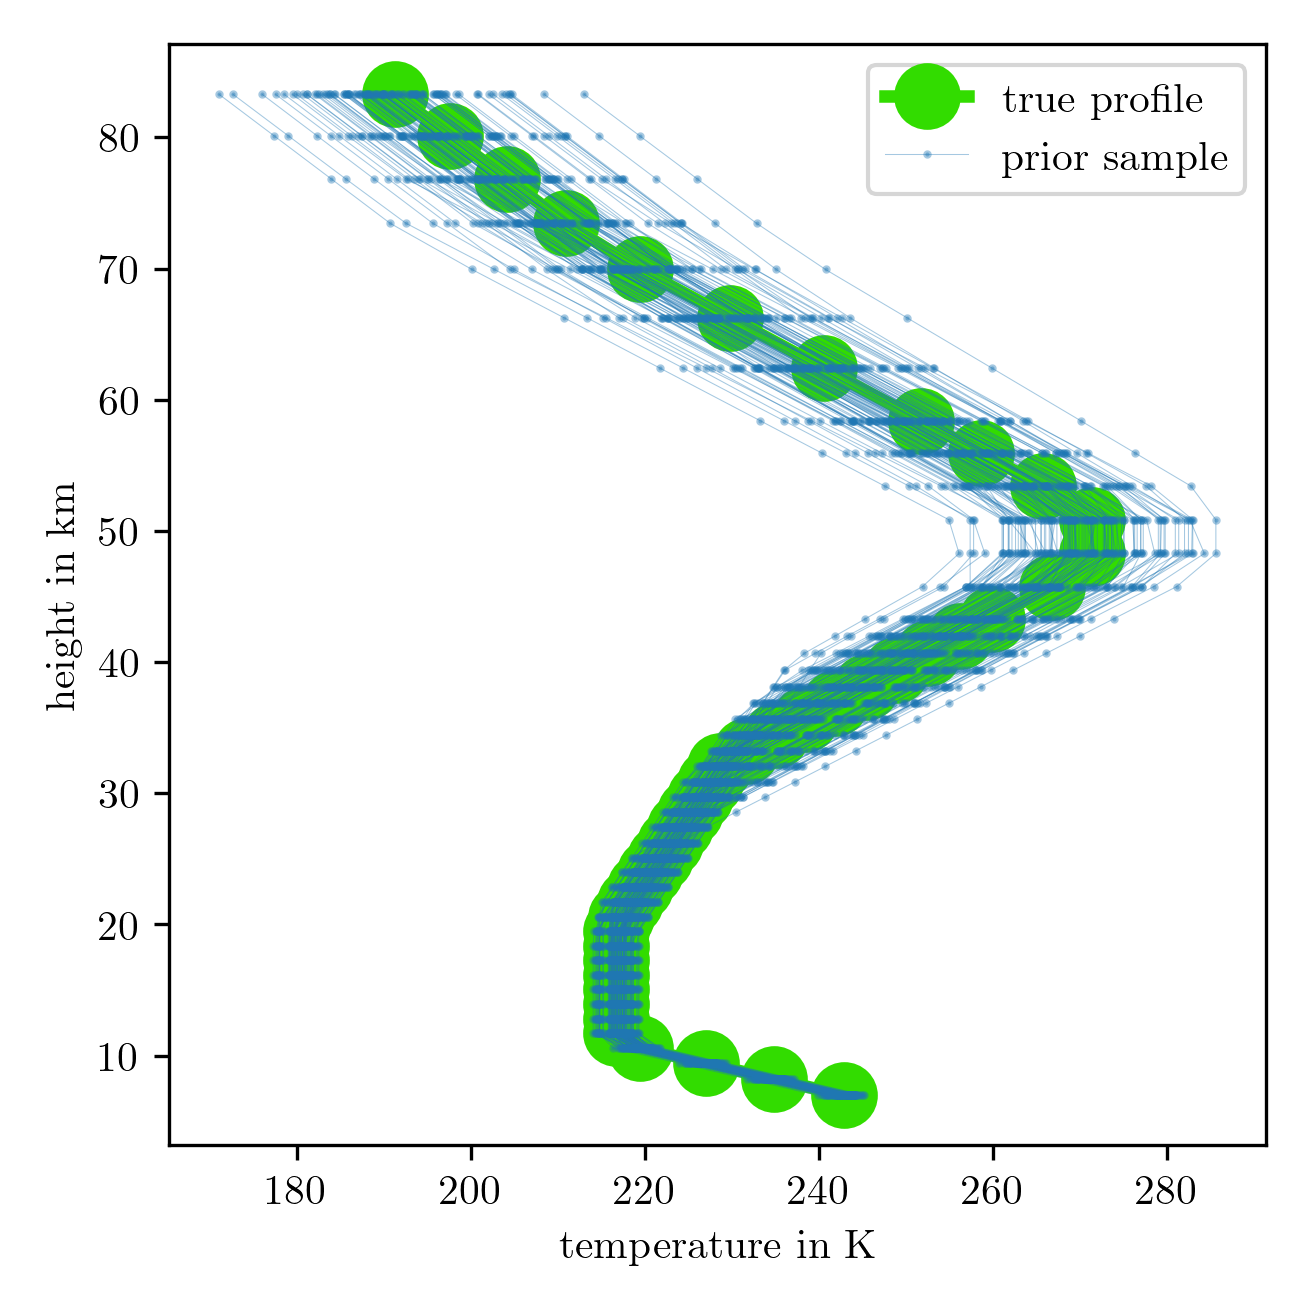
\includegraphics{PriorTempPostMeanSigm.png}
	\caption[Prior Samples of $\bm{T}$ according to the respective hyper-prior distribution.]{We draw samples from the hyper-prior distribution of $h_1, h_2,h_3,h_4,h_5,h_6, a_0, a_1, a_2,a_3,a_4$ and $T_0$ as defined in table \ref{tab:priors} and then calculate $\bm{T}$ according to the function in Eq. \ref{eq:tempFunc}.}
	\label{fig:PriorTemp}
\end{figure}

\begin{figure}[ht!]
	\centering
	\input{TruePress.pdf_tex}
	%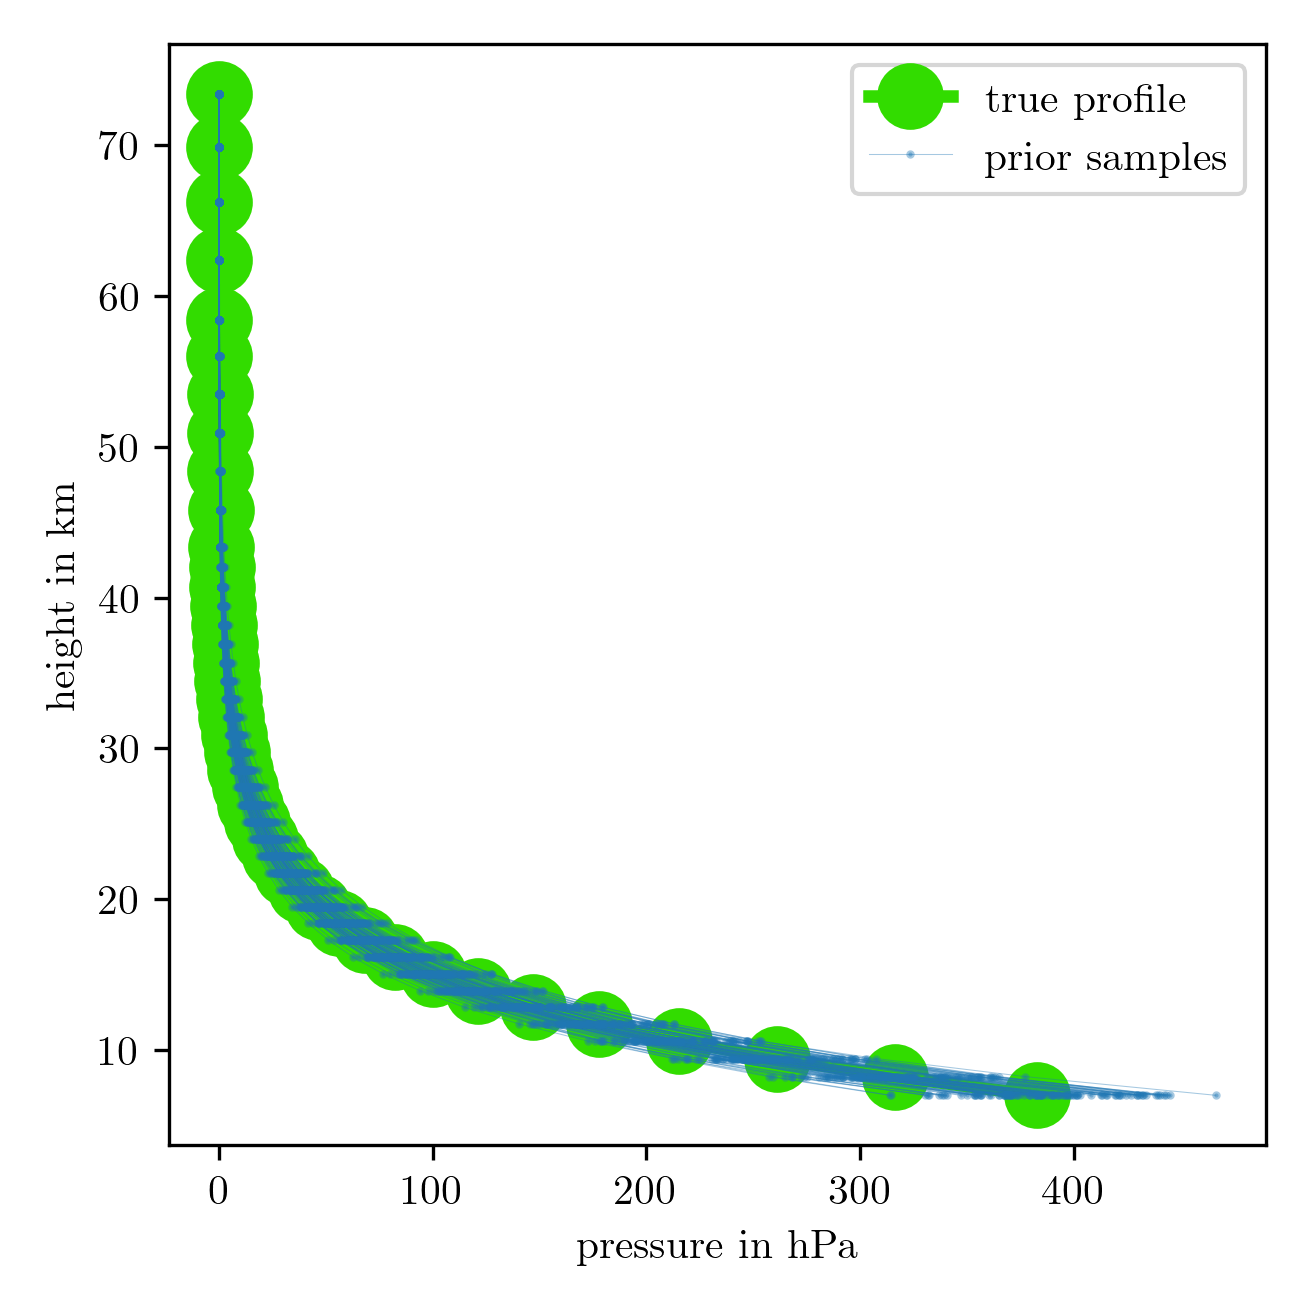
\includegraphics{PriorPressPostMeanSigm.png}
	\caption[Prior Samples of $\bm{p}$ according to the respective hyper-prior distribution.]{We draw samples from the hyper-prior distribution of $h_0, b$ and $p_0$ as defined in table \ref{tab:priors} and then calculate $\bm{p}$ according to the function in Eq. \ref{eq:pressFunc}.}
	\label{fig:PriorPress}
\end{figure}
\begin{figure}[ht!]
	\centering
	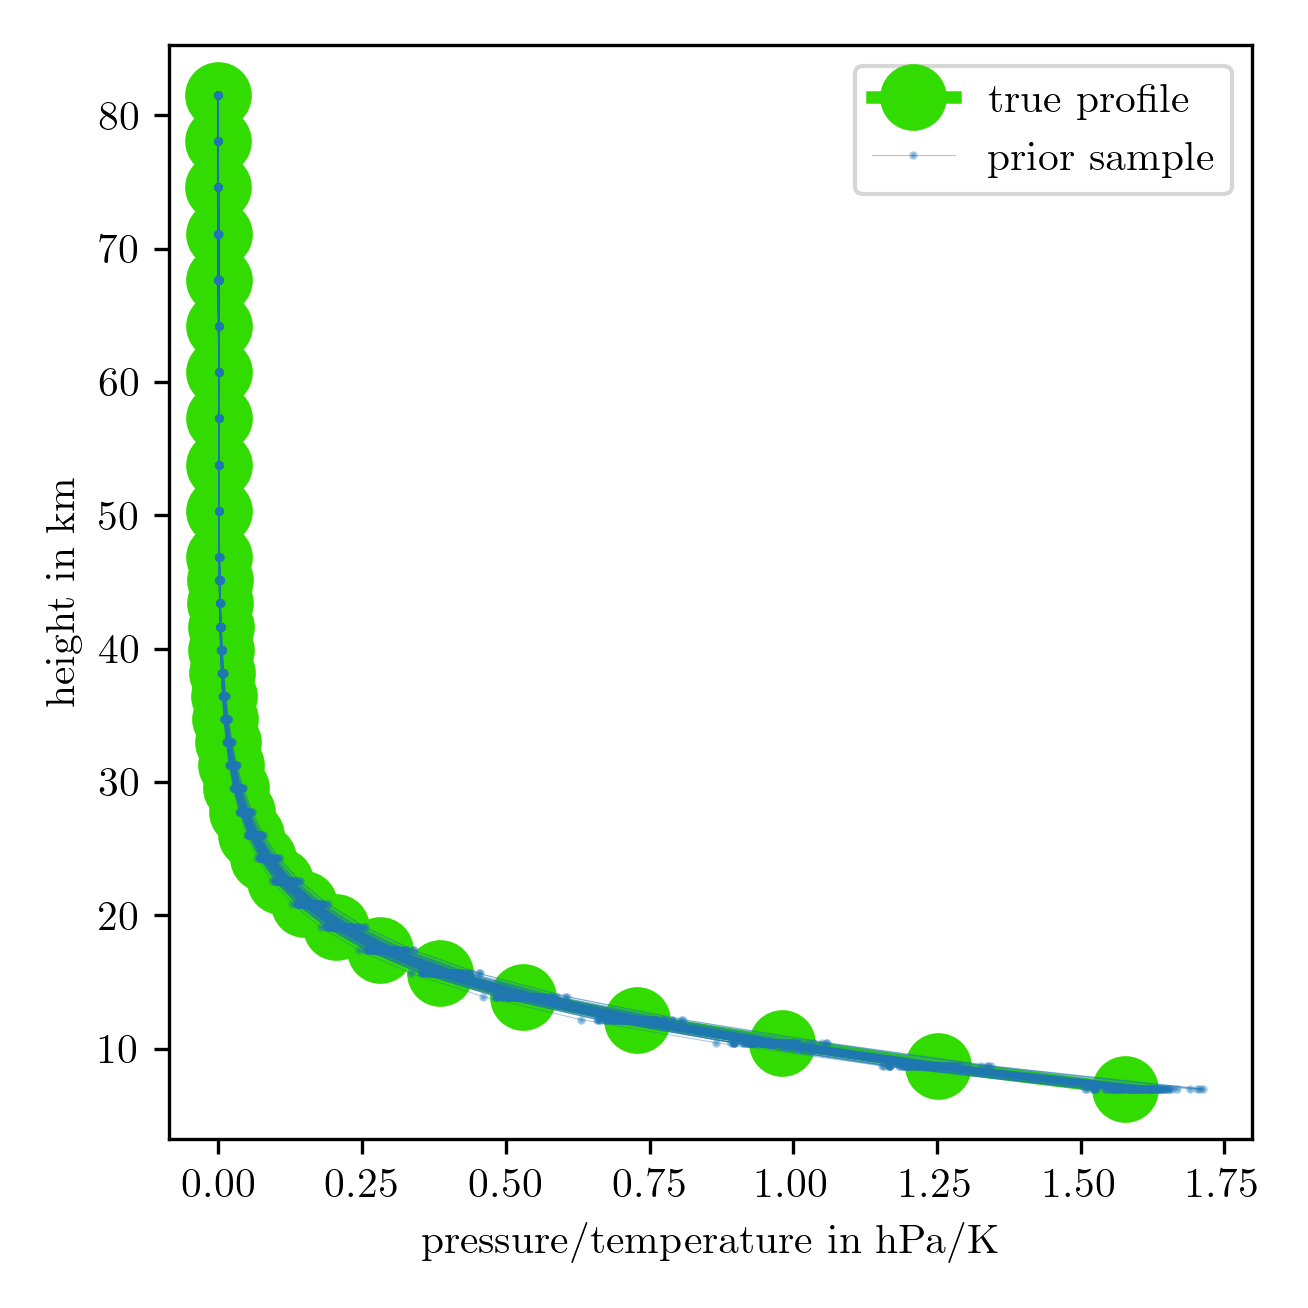
\includegraphics{PriorTempOverPostMeanSigm.png}
	\caption[Prior Samples of $\bm{p}/\bm{T}$ according to the respective hyper-prior distribution.]{We draw samples from the hyper-prior distribution of $h_0, b, p_0, h_1, h_2,h_3,h_4,h_5,h_6, a_0, a_1, a_2,a_3,a_4$ and $T_0$ as defined in table \ref{tab:priors} and then calculate $\bm{p}/\bm{T}$ according to the functions in Eq. \ref{eq:pressFunc} and \ref{eq:tempFunc}.}
	\label{fig:PriorPressOverTemp}
\end{figure}
We plot prior samples of the pressure $\bm{p}$ in Fig. \ref{fig:PriorPress}, the temperature $\bm{T}$ in Fig. \ref{fig:PriorTemp} and the ratio $\bm{p}/\bm{T}$ in Fig. \ref{fig:PriorPressOverTemp} against the ground truth profiles.
Additionally, we plot prior samples of $1/\bm{T}$ in Fig. \ref{fig:OverTempPrior}.
Here we already observe that $\bm{p}/\bm{T}$ inherits the structure of the pressure function and hence the data is uninformative about the temperature, and that is one of the reasons why we chose those normally, rather informative, hyper-prior distributions.
\clearpage

\subsection{Posterior Distribution}
Here, we define the marginal and then conditional posterior distribution for the described Bayesian model.
We either use the \texttt{t-walk} algorithm \cite{christen2010general} to draw samples from $\pi(p_0,b,\bm{h_T},\bm{c_T},\bm{a_T} ,\delta, \gamma| \bm{y})$ or we utilise a TT approximation on a predefined grid to draw samples via the SIRT method with an MH correction step from that marginal posterior.
We define $\bm{\theta}_{\bm{p}, \bm{T}} \coloneqq \{p_0,b,\bm{h_T},\bm{c_T},\bm{a_T}\}$, which includes all hyper-parameters related to pressure and temperature, for brevity.
Lastly, we use the RTO Method to draw samples from the conditional $\pi(\bm{x}|p_0,b,\bm{h_T},\bm{c_T},\bm{a_T} ,\delta, \gamma, \bm{y})$.

\subsubsection{Marginal Posterior Distribution}
The marginal posterior is given as
\begin{align}
	\pi( \lambda,\bm{\theta}_{\bm{p}, \bm{T}},\gamma  | \bm{y}) \propto &  \lambda^{n/2} \gamma^{m/2}   \exp{ \Bigl\{ - \frac{1}{2} g ( \lambda,\bm{\theta}_{\bm{p}, \bm{T}}) - \frac{\gamma}{2} f ( \lambda,\bm{\theta}_{\bm{p}, \bm{T}}) \Bigr\}} \pi(\lambda,\bm{\theta}_{\bm{p}, \bm{T}},\gamma ) \, ,
	\label{eq:MargPostFull}
\end{align}
with $\lambda= \delta / \gamma$,
\begin{subequations}
	\label{eq:fandg}
	\begin{align}
		&f ( \lambda,\bm{\theta}_{\bm{p}, \bm{T}}) = \bm{y}^T \bm{y} - \big(\bm{A}(\bm{\theta}_{\bm{p}, \bm{T}})^T \bm{y}\big)^T \big(\bm{A}(\bm{\theta}_{\bm{p}, \bm{T}})^T  \bm{A}(\bm{\theta}_{\bm{p}, \bm{T}}) + \lambda \bm{L}\big)^{-1} \big(\bm{A}(\bm{\theta}_{\bm{p}, \bm{T}})^T \bm{y}\big)  \label{eq:fAppl} \, ,  \\
		&\text{and } g(\lambda,\bm{\theta}_{\bm{p}, \bm{T}}) = \log \det \big(\bm{A}(\bm{\theta}_{\bm{p}, \bm{T}})^T  \bm{A}(\bm{\theta}_{\bm{p}, \bm{T}}) + \lambda \bm{L}\big) \label{eq:gAppl} \, .
	\end{align}
\end{subequations}
Here we use the approximated forward model $\bm{A}(\bm{\theta}_{\bm{p}, \bm{T}}) \coloneqq \bm{M}\bm{A}(\bm{\theta}_{\bm{p}, \bm{T}})_L$ and do not approximate $f$ and $g$ but calculate $\bm{A}(\bm{\theta}_{\bm{p}, \bm{T}})$ for each function evaluation directly.


\paragraph{Sampling from Marginal Posterior}
For a ground truth, we run the \texttt{t-walk} \cite{christen2010general} algorithm on $\pi( \lambda,\bm{\theta}_{\bm{p}, \bm{T}},\gamma  | \bm{y})$ for $N = 1000 \times 1000$ steps with a burn-in period of $N_{\text{burn-in}} = 100 \times 1000 $, since we expect a maximal IATC, through some pre-analysis, of around $\tau_{\text{int,max}} = 500$, see Tab. \ref{tab:priors}, to generate around $1000$ independent samples from the posterior.
We initialise the Python implementation of the \texttt{t-walk}\cite{christentwalkaccess} around the hyper-prior mean values and take a total number of $N' =N + N_{\text{burn-in}} = 1100000$ steps around $5$ mins.
We iteratively define the TT grid according to the results of the \texttt{t-walk}, and also use these boundaries for the hyper-parameters when running the \texttt{t-walk} (see Tab. \ref{tab:priors}).
We plot the resulting histograms in Fig. \ref{fig:PostHistTT0} to \ref{fig:PostHistTT4} and the trace of the samples in Fig. \ref{fig:TraceTwalk}.

\paragraph{TT Approximation of Marginal Posterior}
The aim now is to approximate the square root of the marginal posterior
\begin{align}
	\begin{split}
		\pi( \lambda,\bm{\theta}_{\bm{p}, \bm{T}},\gamma  | \bm{y}) \propto  \exp\Bigl\{\log{\pi( \lambda,\bm{\theta}_{\bm{p}, \bm{T}},\gamma  | \bm{y}) ) } + c \Bigr\}  
	\end{split} \, ,
	\label{eq:MargPostFullTT}
\end{align}
where we introduce a "normalisation constant" $c=-100$, similar to Sec. \ref{subsec:FirstMTC}, to avoid under or overflow.
In doing so we run the \texttt{tt.cross.rectcross.rect\_cross.cross} function from the \texttt{ttpy} python package \cite{Oseledets2018ttpy}.
We compute the marginal as in Sec. \ref{sec:tensortrain}, where we set $\xi = 1 / \uplambda (\mathcal{X})$ and $\uplambda(x) = 1$ so that for Cartesian basis $\bm{M}_k = \text{diag}(\uplambda_k(\mathcal{X}_k))$.
To draw samples from this TT approximation we use the SIRT-MH scheme as in Sec. \ref{}


\subparagraph{Correlation structure}
First, we arrange the order of hyper-parameters according to their correlation structure to make the TT approximation more efficient.
In doing so, highly correlated hyper-parameter pairs are next each other, so that their TT cores are direct neighbours and linked through their shared rank.
See Fig.\ref{fig:CorrPlot}, where we scatter plot the samples from the TT approximation of $\sqrt{\pi(p_0,b,T_0,\bm{h_T},\bm{a_T} | \bm{y}, \gamma, \bm{x})}$ via SIRT-MH scheme and plot the Pearson correlation coefficient.
A coefficient close to $1$ or $-1$ corresponds to high correlation, whereas low correlation between hyper-parameters has a coefficient close to zero.
We observe that the $\lambda$ hyper-parameters is highly correlated with $b$ the hyper-parameter describing the pressure gradient and with $\gamma$.
Additionally, $h_{T,1}$ and $T_0$ describing the temperature at low altitudes are correlated to $b$ as well, since those do very slightly influence "the smoothness" of $\bm{p}/\bm{T}$, hard to see in Fig. \ref{fig:PriorPressOverTemp}.
The IACTs in Tab. \ref{tab:priors} agree with these results.
Note that the correlation for parameters describing temperature in higher altitudes and surprisingly $p_0$ are very much uncorrelated.
Next we aim to find the optimal rank and grid size to approximate $\sqrt{\pi(p_0,b,T_0,\bm{h_T},\bm{a_T} | \bm{y}, \gamma, \bm{x})}$, so that the number of function evaluation is as low as possible without too much sacrifice in accuracy.
\begin{figure}[h]% will be the left-side figure
	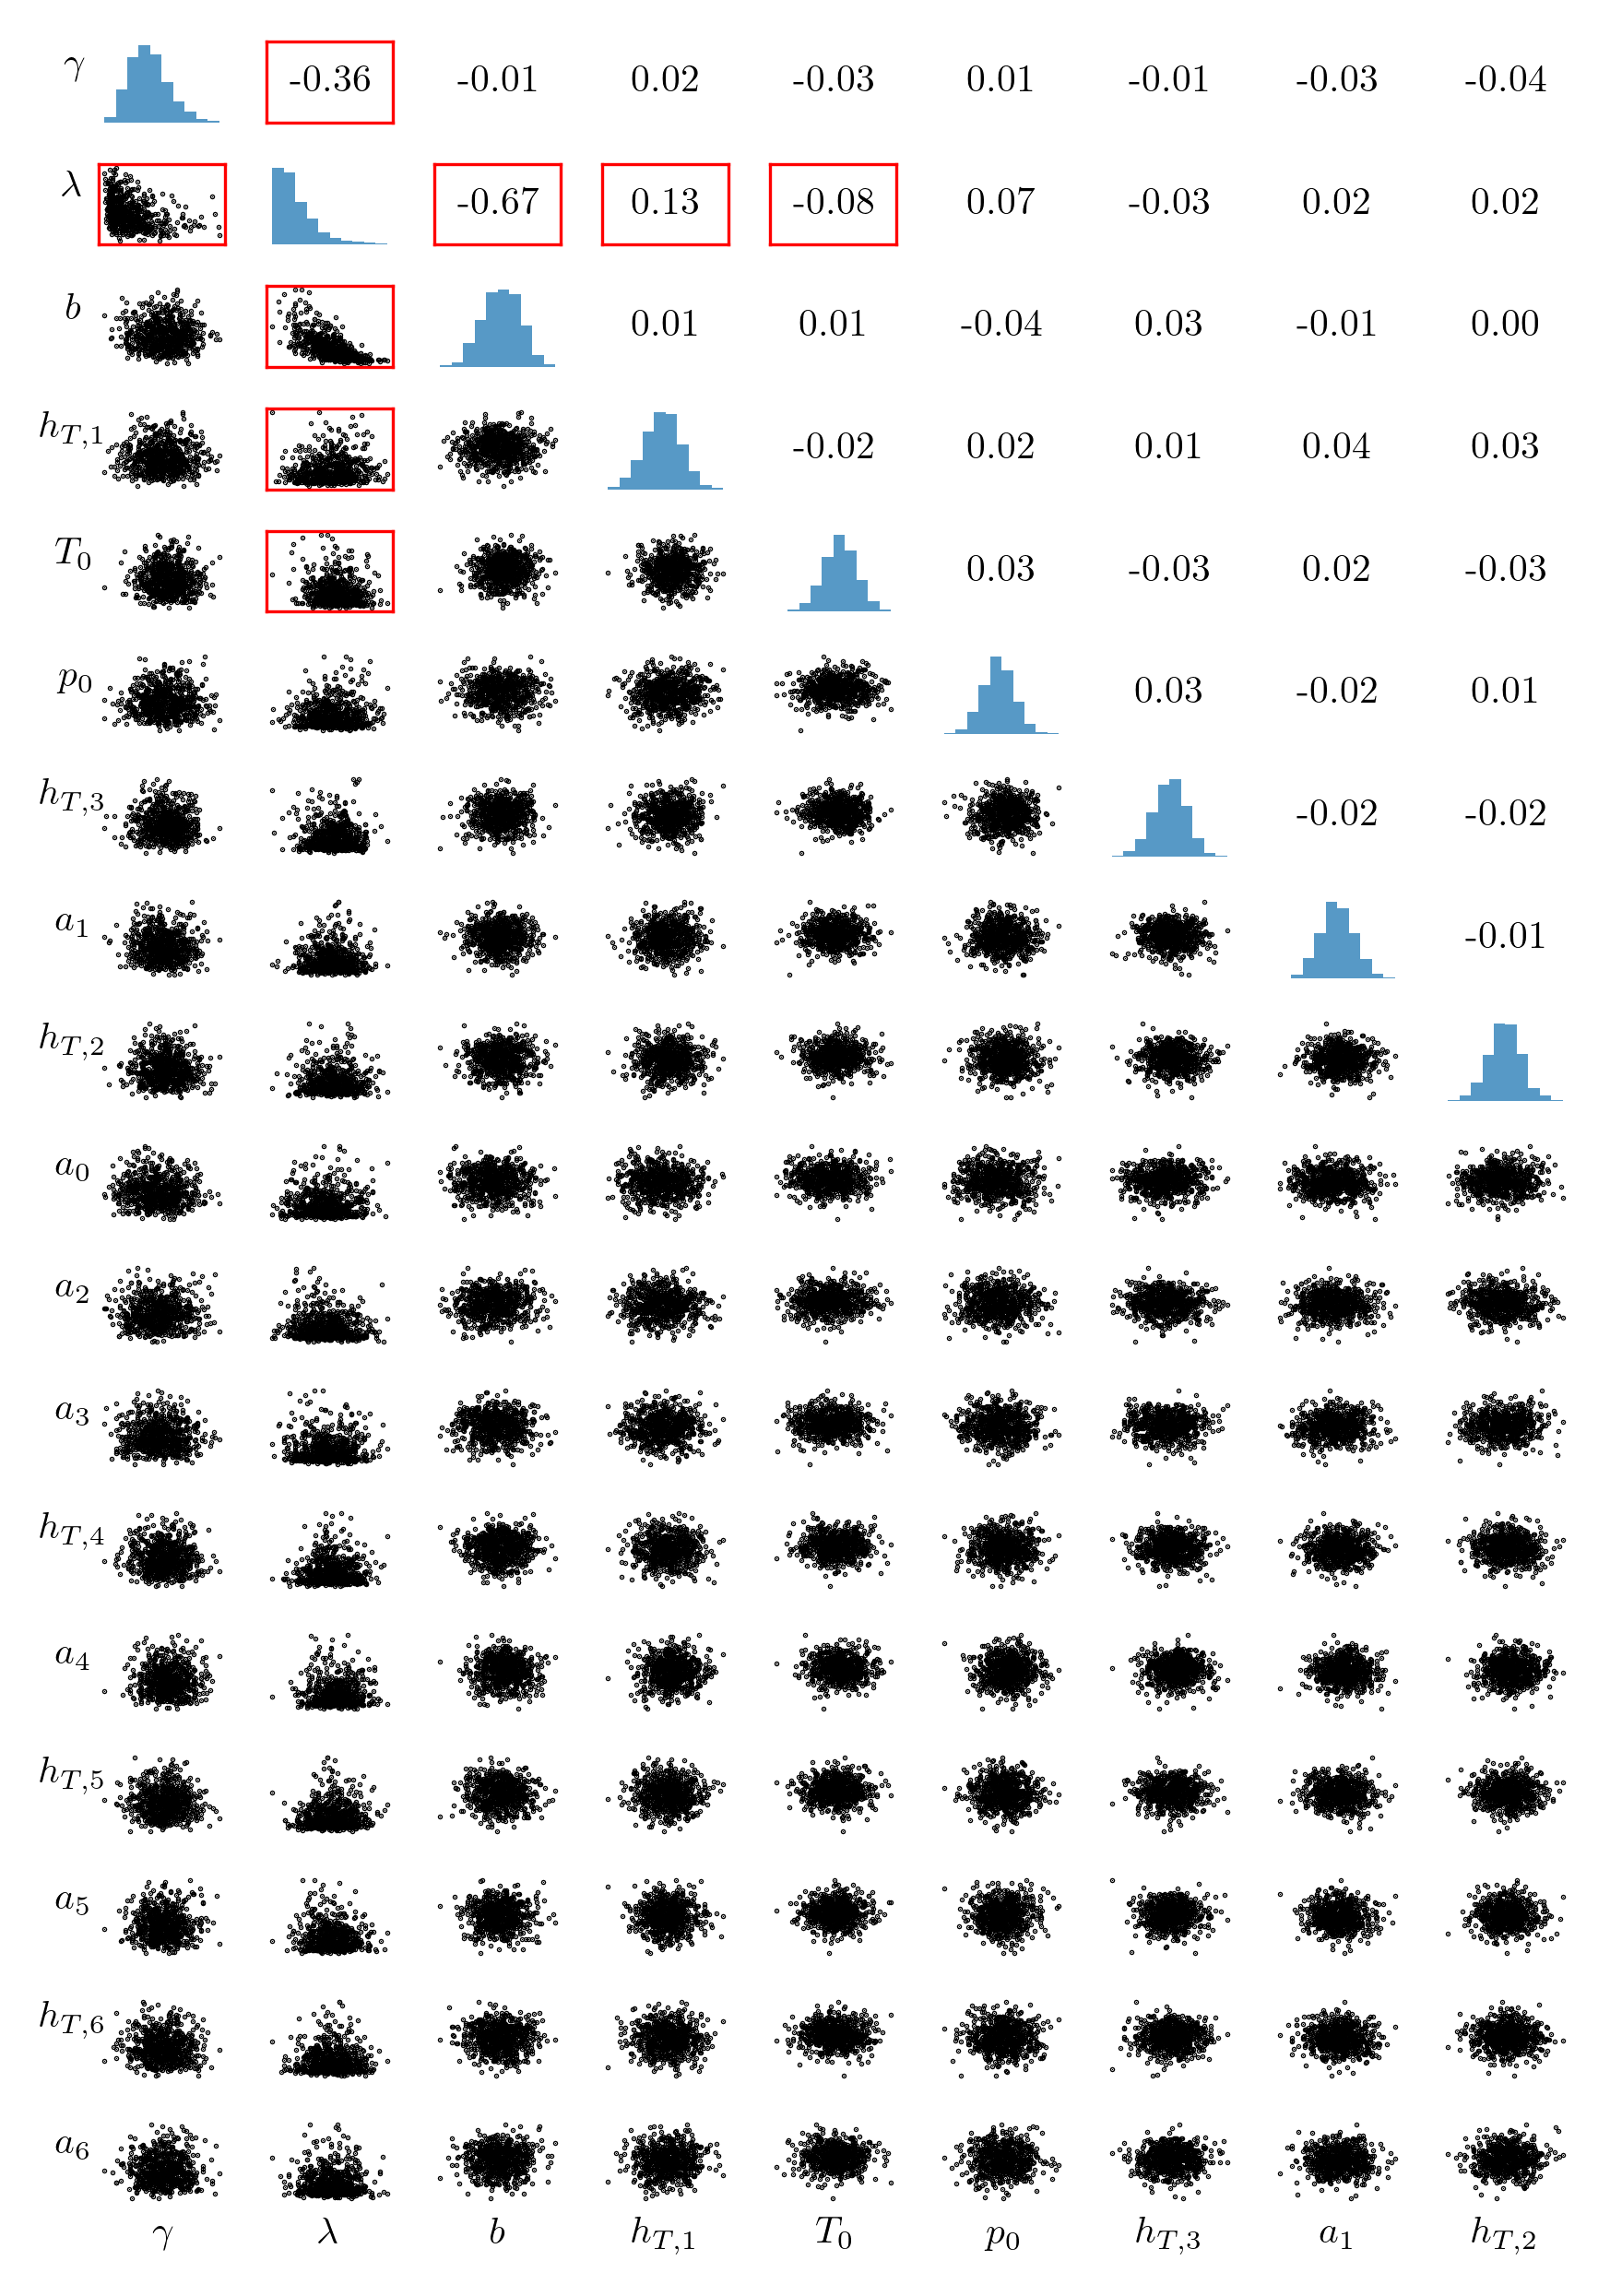
\includegraphics[]{CorrPlot.png}
	\caption[Correlation plot of samples from TT-approximation]{Scatter plot of samples from TT-approximation of $\sqrt{\pi(p_0,b,T_0,\bm{h_T},\bm{a_T} | \bm{y}, \gamma, \bm{x})}$ via SIRT scheme. We plot the Pearson correlation coefficient ranging from $-1$ to $1$ for each hyper-parameter pair.}
	\label{fig:CorrPlot}
\end{figure}
\begin{figure}% will be the right-side figure
	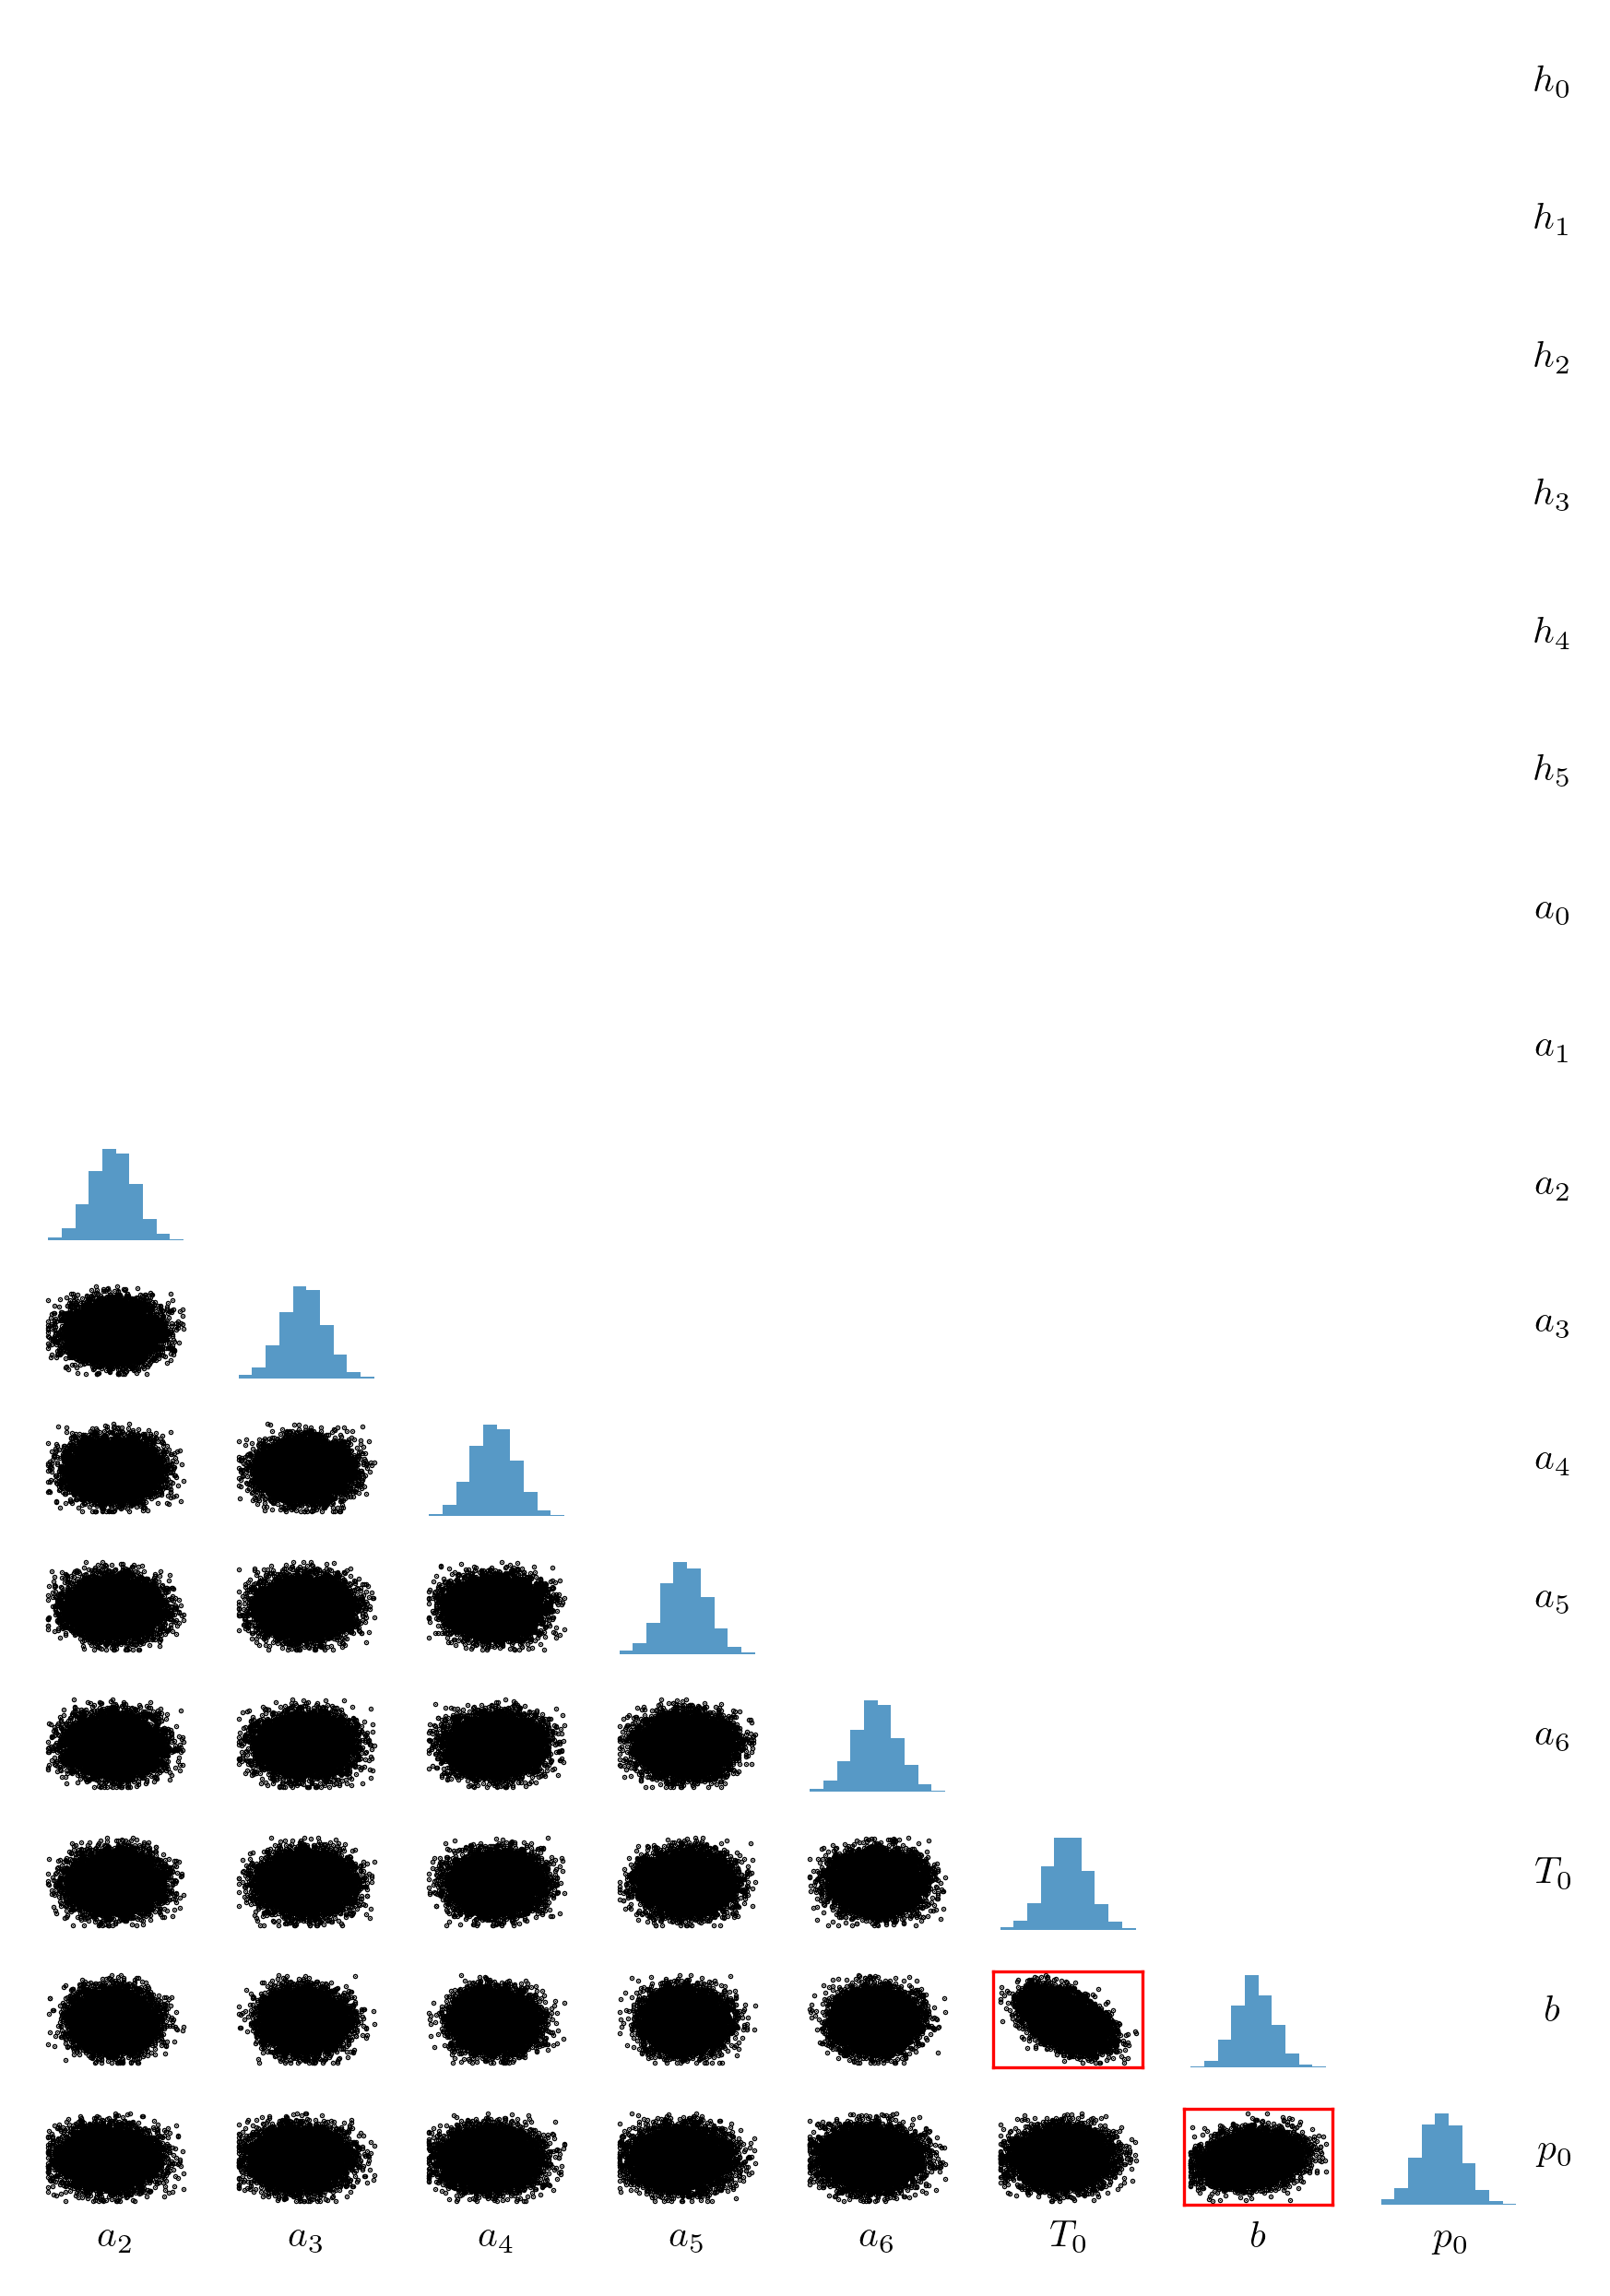
\includegraphics[]{2ndCorrPlot.png}
	\caption*{Correlation plot of samples from TT-approximation of $\sqrt{\pi(p_0,b,T_0,\bm{h_T},\bm{a_T} | \bm{y}, \gamma, \bm{x})}$ via SIRT scheme.}
\end{figure}
\cleardoublepage


\subparagraph{Find optimal Rank and Grid Size}
Next, we choose a relatively large number of grid points of $n = 150$ and calculate different error measures for deceasing number of ranks to find the optimal number of ranks.
Then we fix a small but tolerable rank and decrease the number of grid points until sufficient accuracy.

We calculate the 1-Wasserstein distance, see Sec. \ref{subsec:wasser}, between $5000$ independent samples from the SIRT-MH scheme, weighted with the TT approximation of marginal posterior, and 4101 independent samples from the \texttt{t-walk}, weighted by the true posterior value.  
To calculate the 1-Wasserstein distance, as in Eq. \ref{eq:applWasser}, we use the \texttt{SamplesLoss("sinkhorn", p=1, blur=0.05, scaling=0.8)} function with default settings from the python package \texttt{geomloss} \cite{Wassersteinaccess}.
This provides the unbiased Sinkhorn divergence which converges towards the Wasserstein distance and can be understood as the generalised Quicksort algorithm \cite{feydy2020OT}.
Here, p = 1 defines the distance measure $\lVert \bm{x} -\tilde{\bm{x}} \rVert_{L^2}$, the blur parameter can be understood as an entropic penalty and the  scaling parameter specifies the trade-off between speed (scaling < .4) and accuracy (scaling > .9) \cite{Wassersteinaccess}.
Additionally we use the marginal functions of each TT approximation to calculate the weighted means $\bm{\mu}_{\text{TT}} \in \mathbb{R}^{18}$ of each hyper-parameter and then the relative RMS deffierence $\lVert\bm{\mu}_{\text{TT}} - \bm{\mu}_{\texttt{t-walk}} \rVert_{L^2} / \lVert \bm{\mu}_{\texttt{t-walk}} \rVert_{L^2}  $ compared to "true means"  $\bm{\mu}_{\texttt{t-walk}}$from the \texttt{t-walk}.
Additionally, we compare the mean $\bm{\mu}_{\text{SIRT-MH}}$ based on the samples from the SIRT-MH scheme with the "true" \texttt{t-walk} mean.
We plot all of these measures in Fig. \ref{fig:FindRankGrid} and decide that a rank $r = 10$ sufficient because the 1-Wasserstein distance is relatively stable for $r\geq10$.
We decide that a grid size $n = 40$ is large enough based in the relative differences of the samples based and integrated mean compared to the \texttt{t-walk} mean, which also seem to be relatively stable for $n \geq 40$.

\begin{figure}[ht!]% will be the left-side figure
	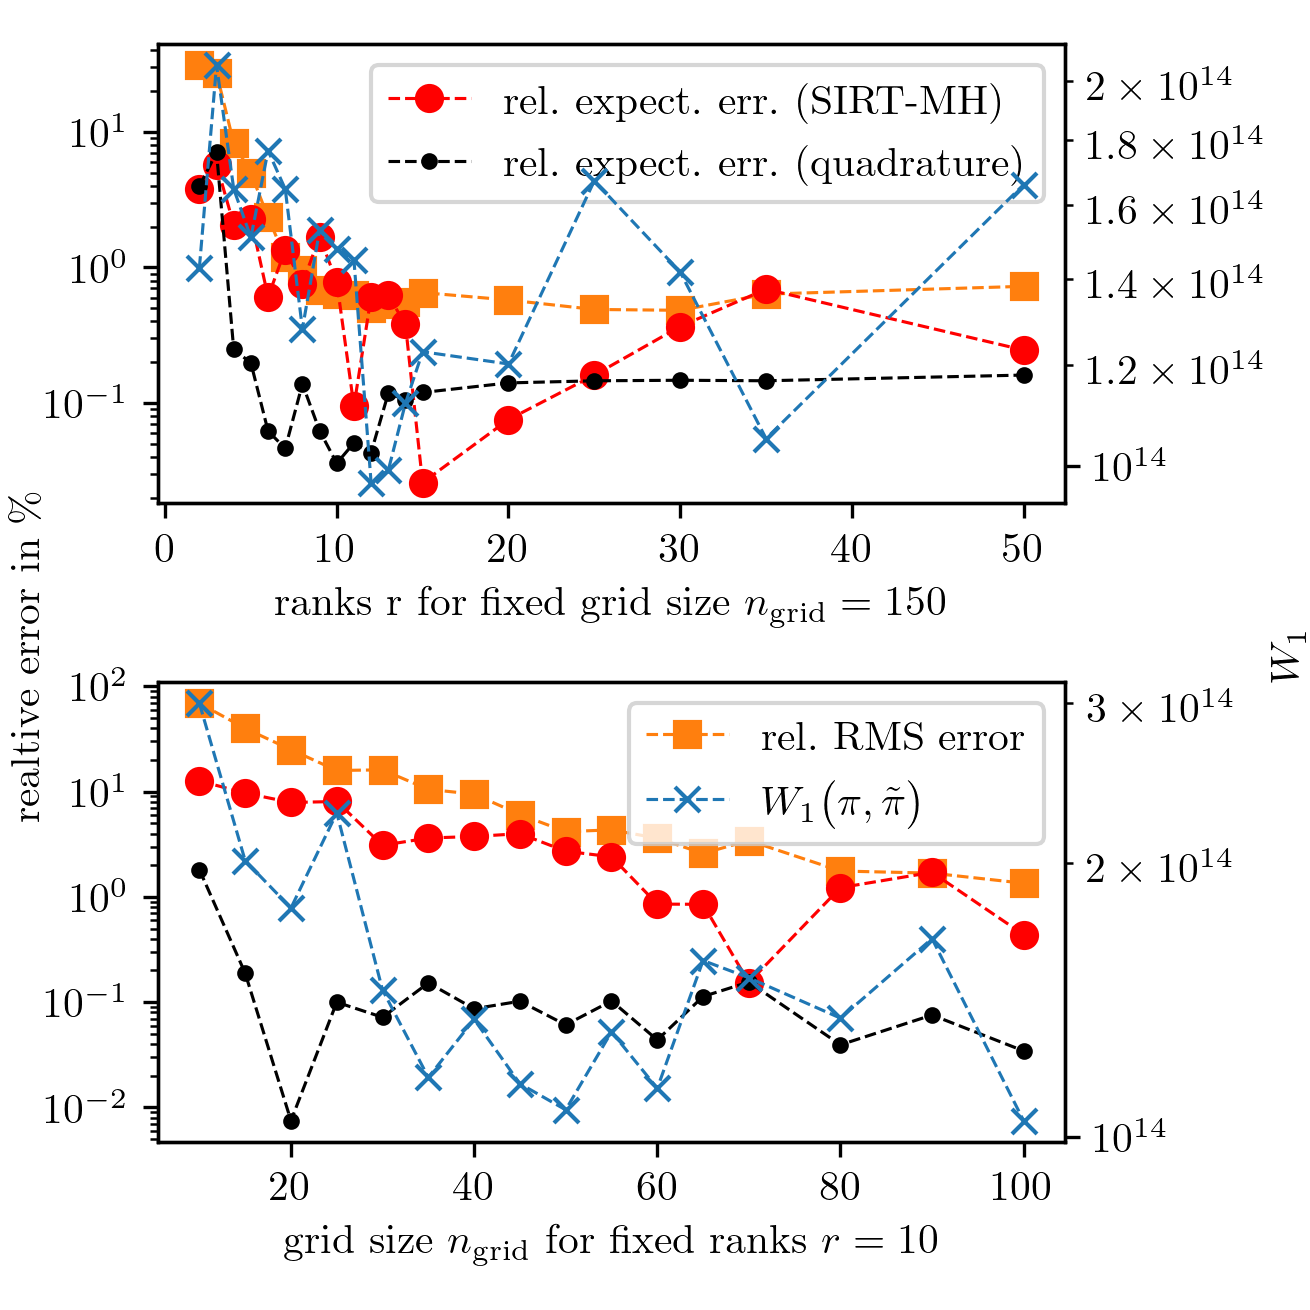
\includegraphics[]{findGridRank.png}
	\caption[Optimal rank and number of grid points for TT approximation.]{Given a TT approximation of $\sqrt{\pi( \lambda,\bm{\theta}_{\bm{p}, \bm{T}},\gamma  | \bm{y}) }$ we calculate the realtive RMS error and the 1-Wasserstein distance between approximated values at sample points provided by the SIRT-MH and the true function values. Further we use the marginal function from the TT approximation to calculate mean values of each hyper-parameter as weighted expectations and compare to the sample mean provided by the \texttt{t-walk}. Additionally we compare sample based mean from the SIRT-MH and the \texttt{t-walk}. We plot the relative RMS difference between those calculations. Note that the y-axis represents the recreative errors related to all measures but $W_1$. We do so since the each hyper-parameters has a different scale we are only interested in the trend of the $W_1$.}
	\label{fig:FindRankGrid}
\end{figure}
\clearpage

To decrease the number of functions evaluation and define ranks $r = [ 1,  10,  10, 10, 10, 10, 5, 5, 5, 5, 5, 3, 2, 2, 2, 2, 2, 2, 1]$ according to the correlation structure of $\pi( \lambda,\bm{\theta}_{\bm{p}, \bm{T}},\gamma  | \bm{y})$ (see Fig. \ref{fig:CorrPlot}).
We need one sweep in \texttt{tt.cross.rectcross.rect\_cross.cross}, reducing the computation time to $\approx0.5$min and the number of functions evaluations to 48240.
Note that we can initialise the \texttt{tt.cross.rectcross.rect\_cross.cross} algorithm at a previously calculated approximation.
We plot the marginals for each hyper-parameter in Fig. \ref{fig:PostHistTT0} to Fig. \ref{fig:PostHistTT5} and samples in Fig. \ref{fig:CorrPlot} .
\begin{figure}[ht!]
	\centering
	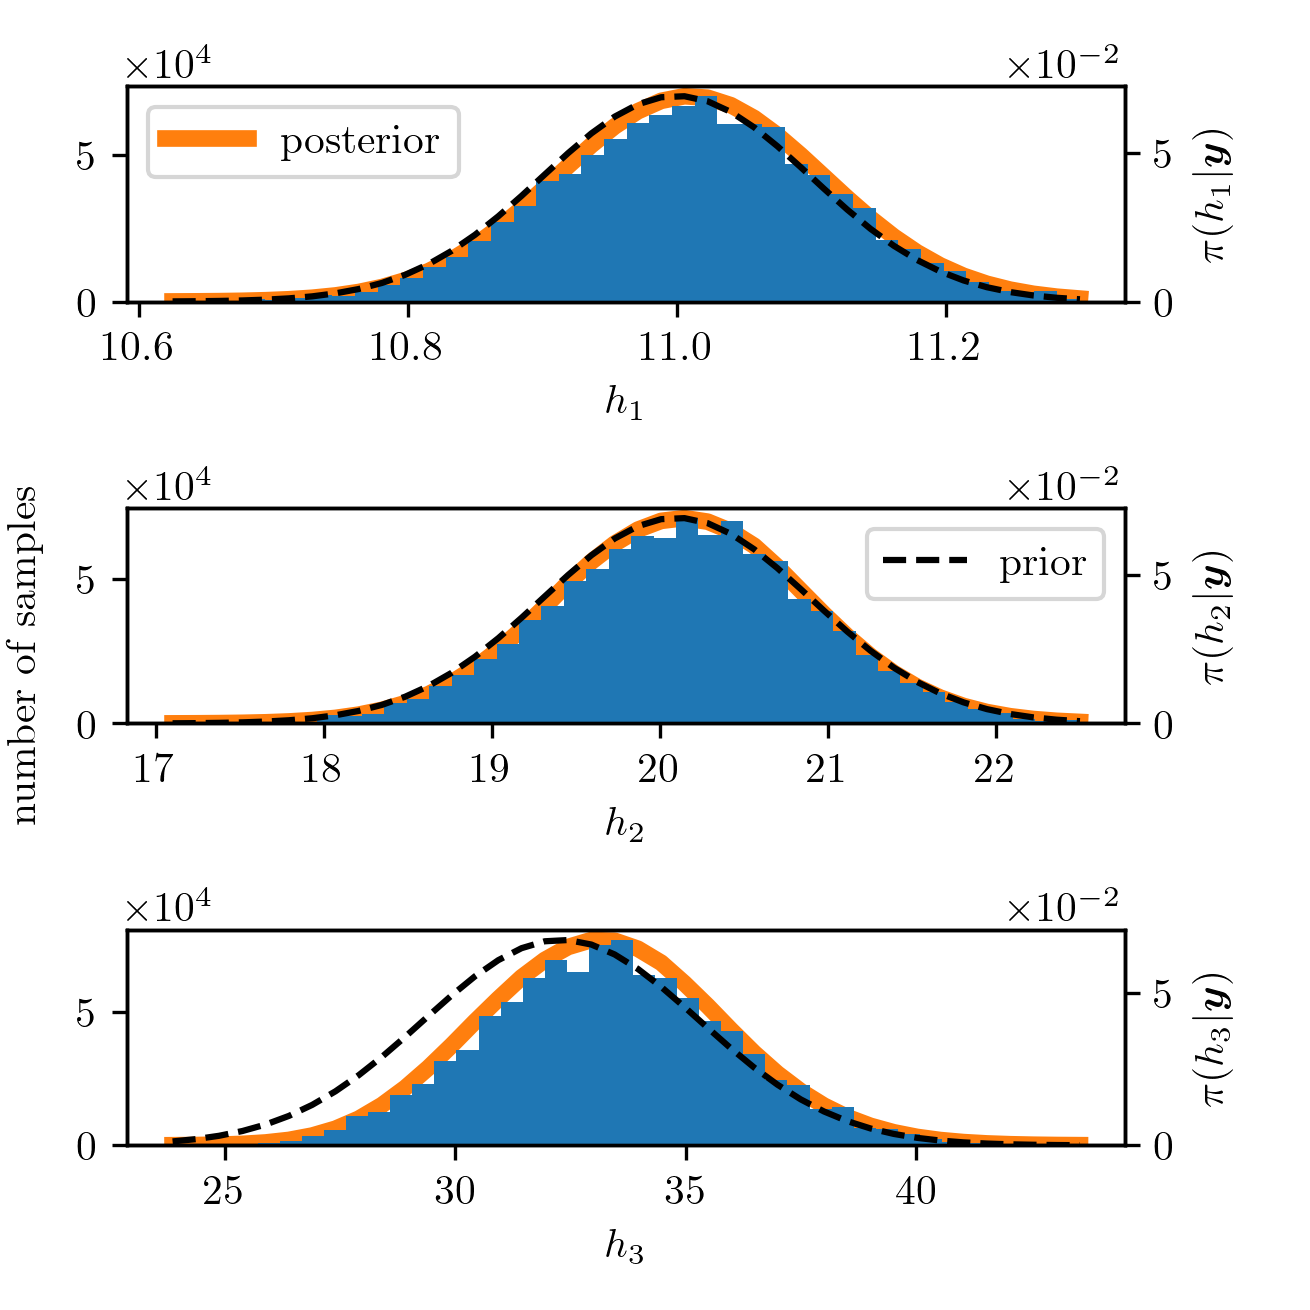
\includegraphics{PHdPTPost0.png}
	\caption[Histograms and TT approximation of posterior distribution as well as hyper-prior distribution.]{We plot the TT approximation of marginal posterior in orange and the samples as a histogram as well as the prior distribution with a dotted line.}
	\label{fig:PostHistTT0}
\end{figure}
\begin{figure}[ht!]
	\centering
	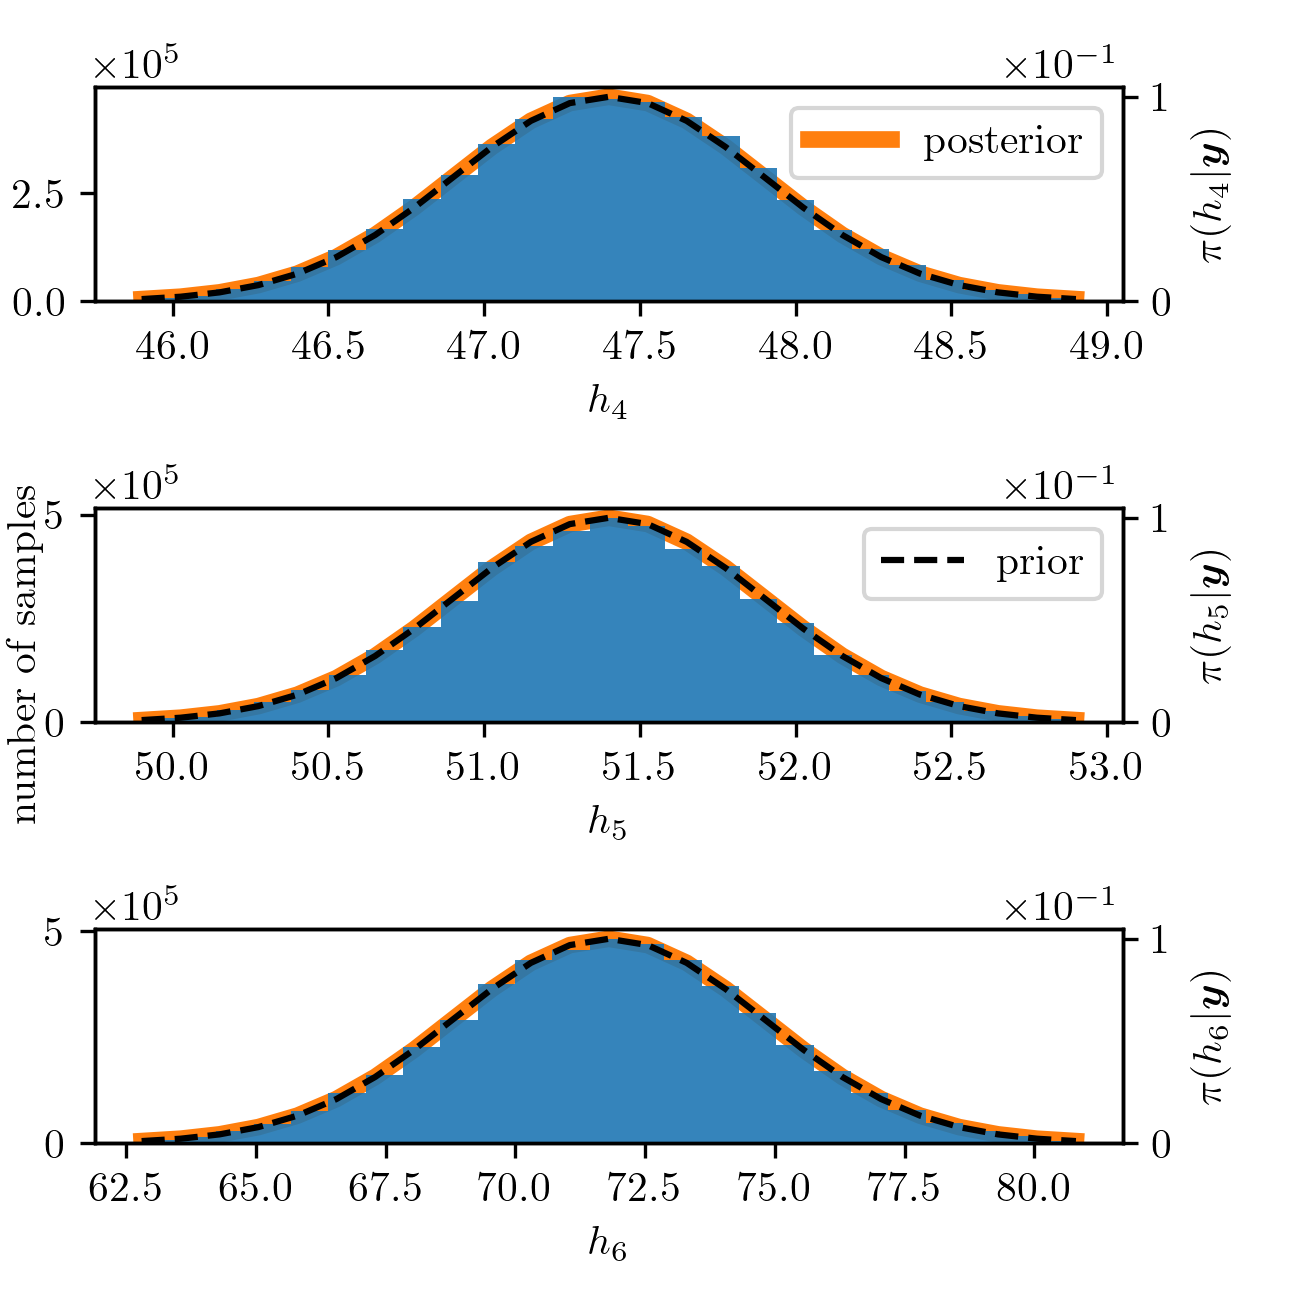
\includegraphics{PHdPTPost1.png}
	\caption[Histograms and TT approximation of posterior distribution as well as hyper-prior distribution.]{We plot the TT approximation of marginal posterior in orange and the samples as a histogram as well as the prior distribution with a dotted line.}
	\label{fig:PostHistTT1}
\end{figure}
\begin{figure}[ht!]
	\centering
	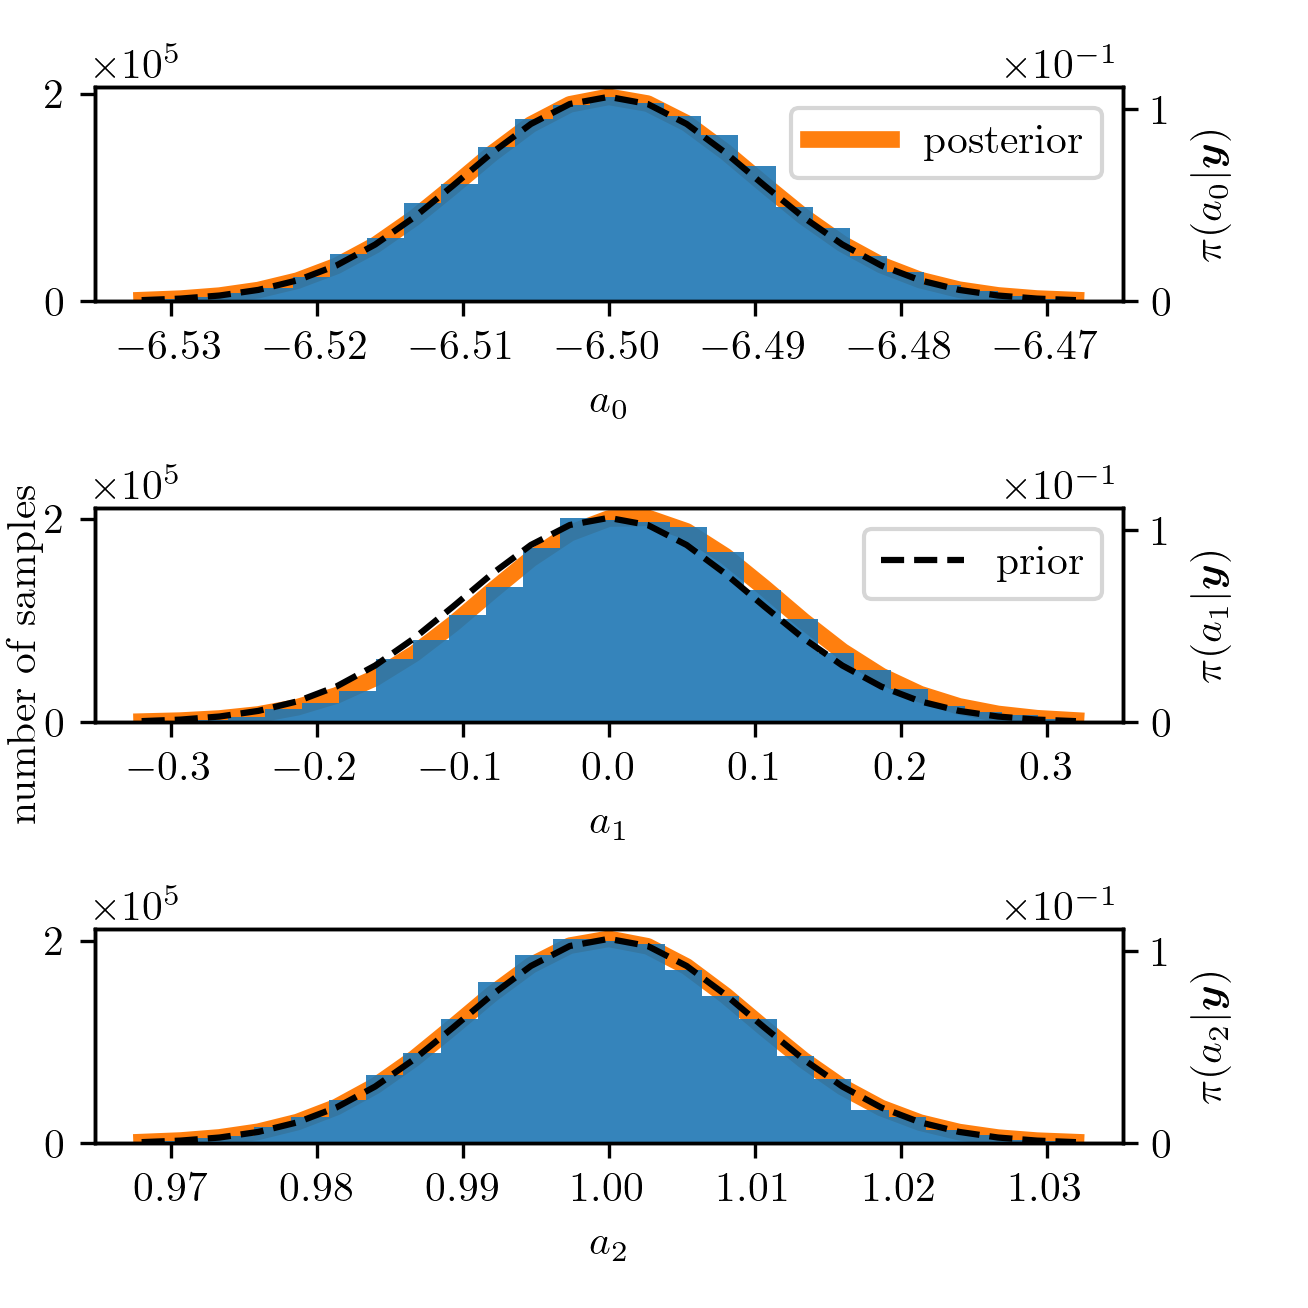
\includegraphics{PHdPTPost2.png}
	\caption[Histograms and TT approximation of posterior distribution as well as hyper-prior distribution.]{We plot the TT approximation of marginal posterior in orange and the samples as a histogram as well as the prior distribution with a dotted line.}
	\label{fig:PostHistTT2}
\end{figure}
\begin{figure}[ht!]
	\centering
	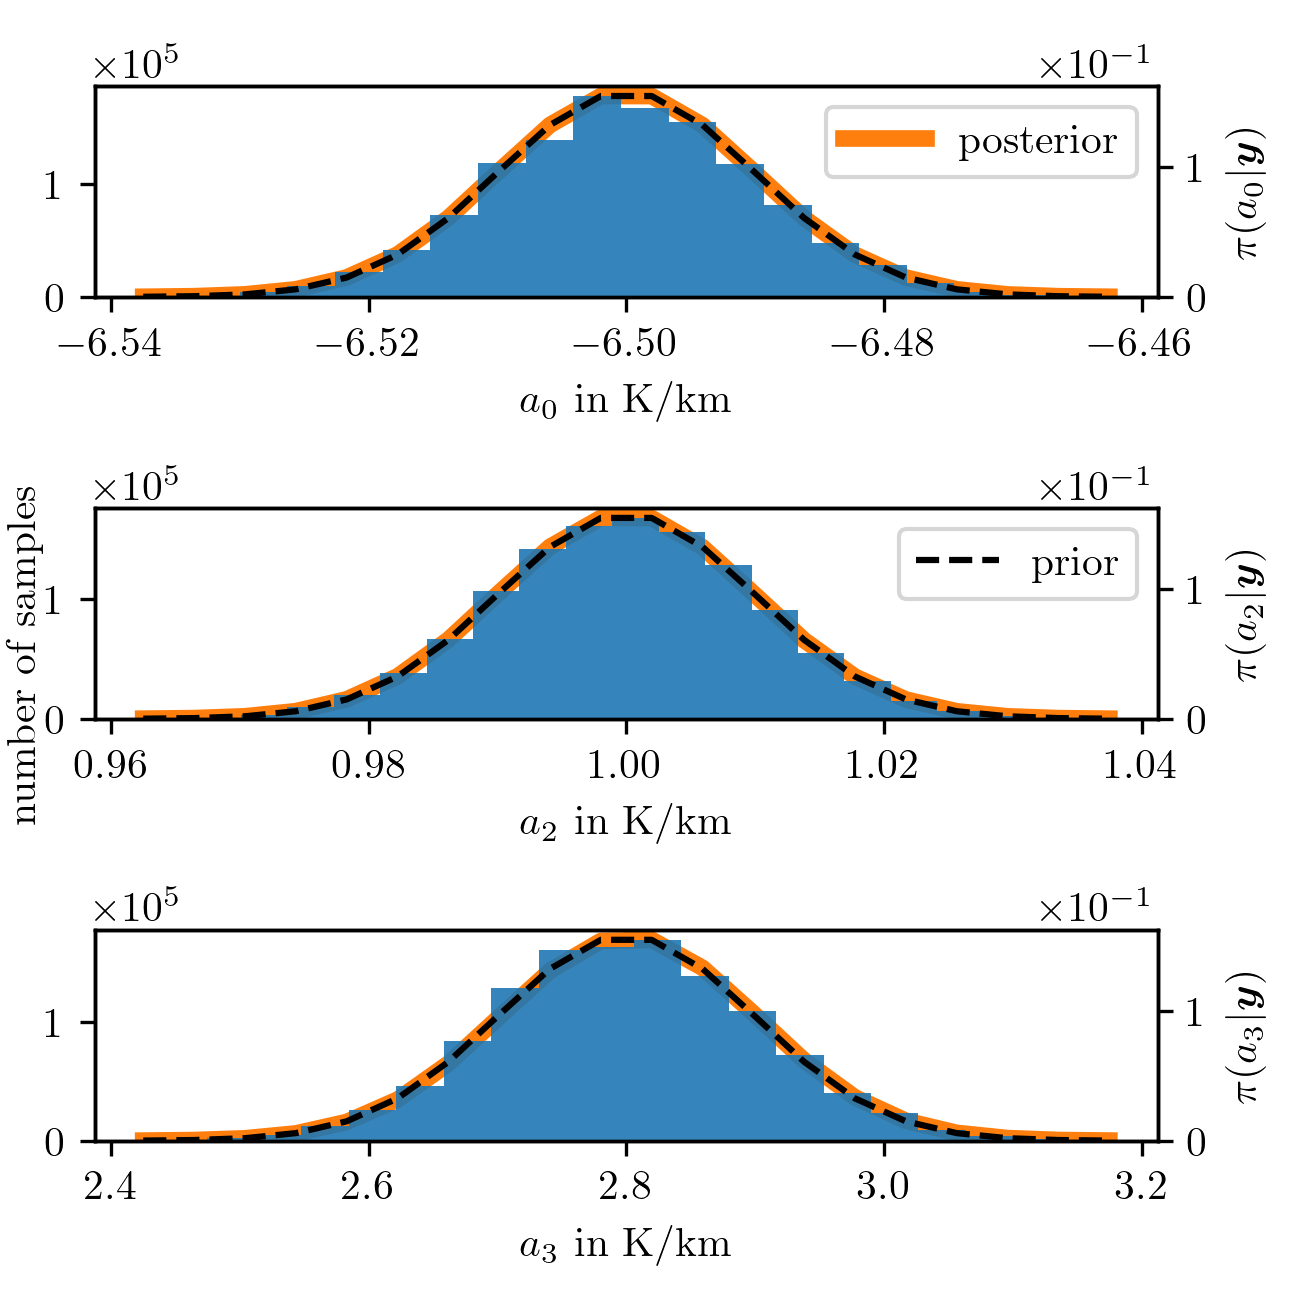
\includegraphics{PHdPTPost3.png}
	\caption[Histograms and TT approximation of posterior distribution as well as hyper-prior distribution.]{We plot the TT approximation of marginal posterior in orange and the samples as a histogram as well as the prior distribution with a dotted line.}
	\label{fig:PostHistTT3}
\end{figure}
\begin{figure}[ht!]
	\centering
	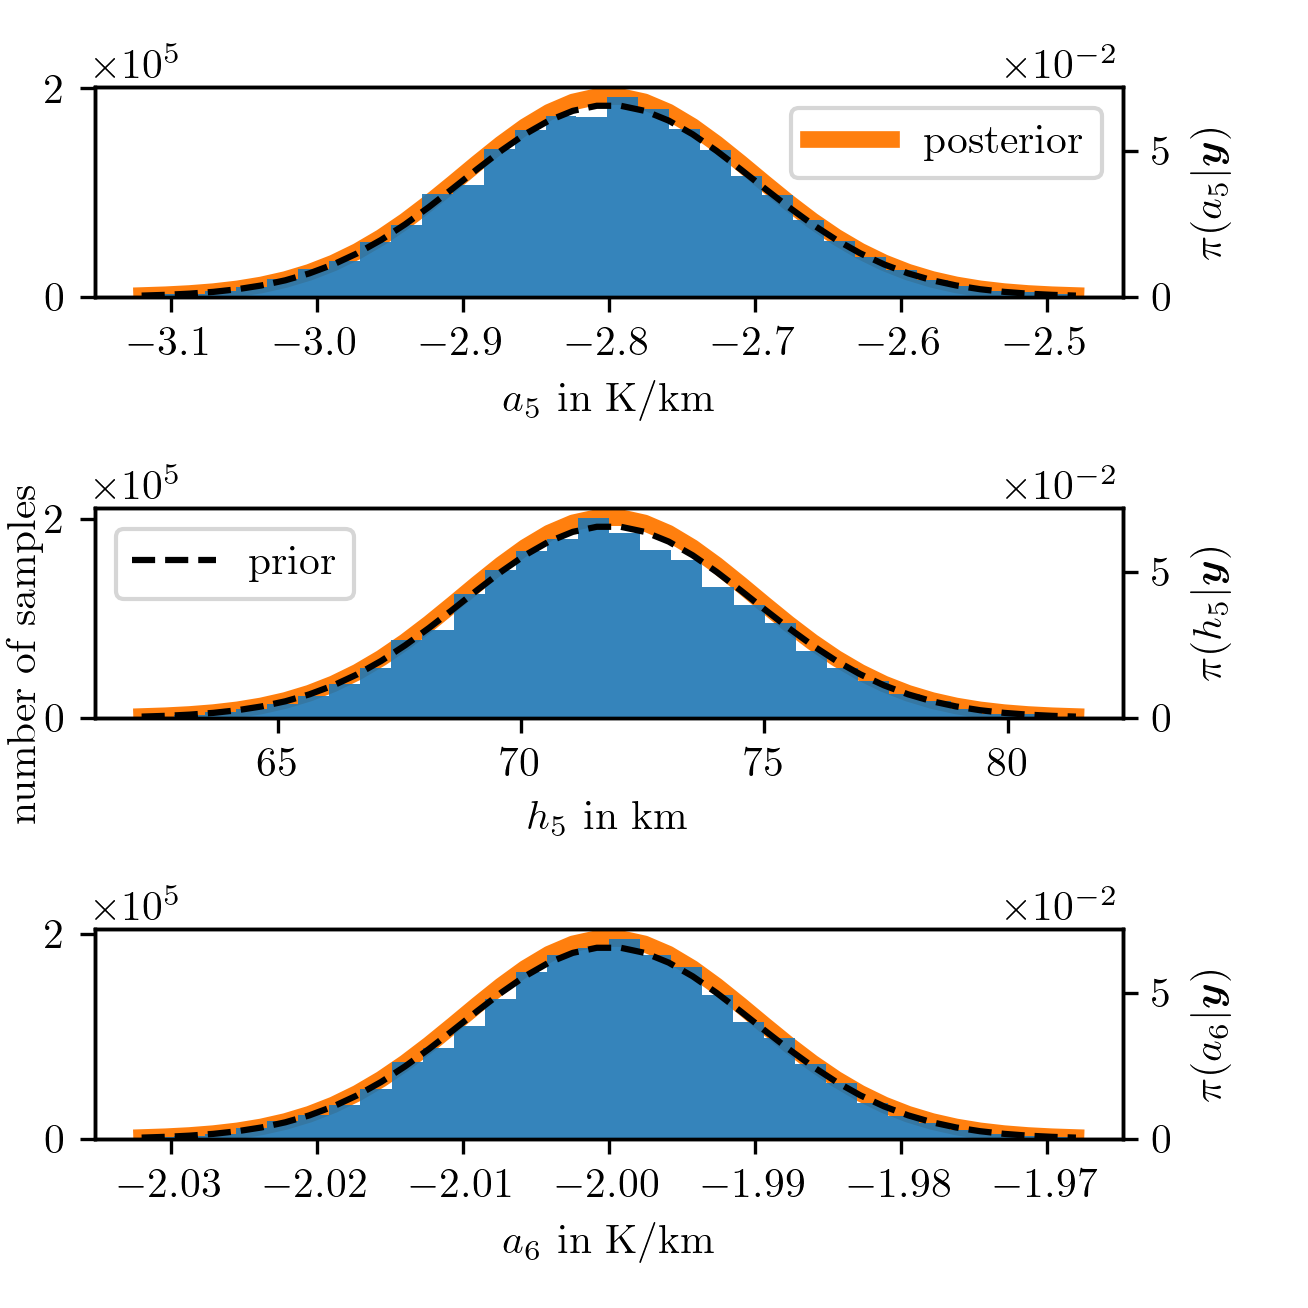
\includegraphics{PHdPTPost4.png}
	\caption[Histograms and TT approximation of posterior distribution as well as hyper-prior distribution.]{We plot the TT approximation of marginal posterior in orange and the samples as a histogram as well as the prior distribution with a dotted line.}
	\label{fig:PostHistTT4}
\end{figure}
\begin{figure}[ht!]
	\centering
	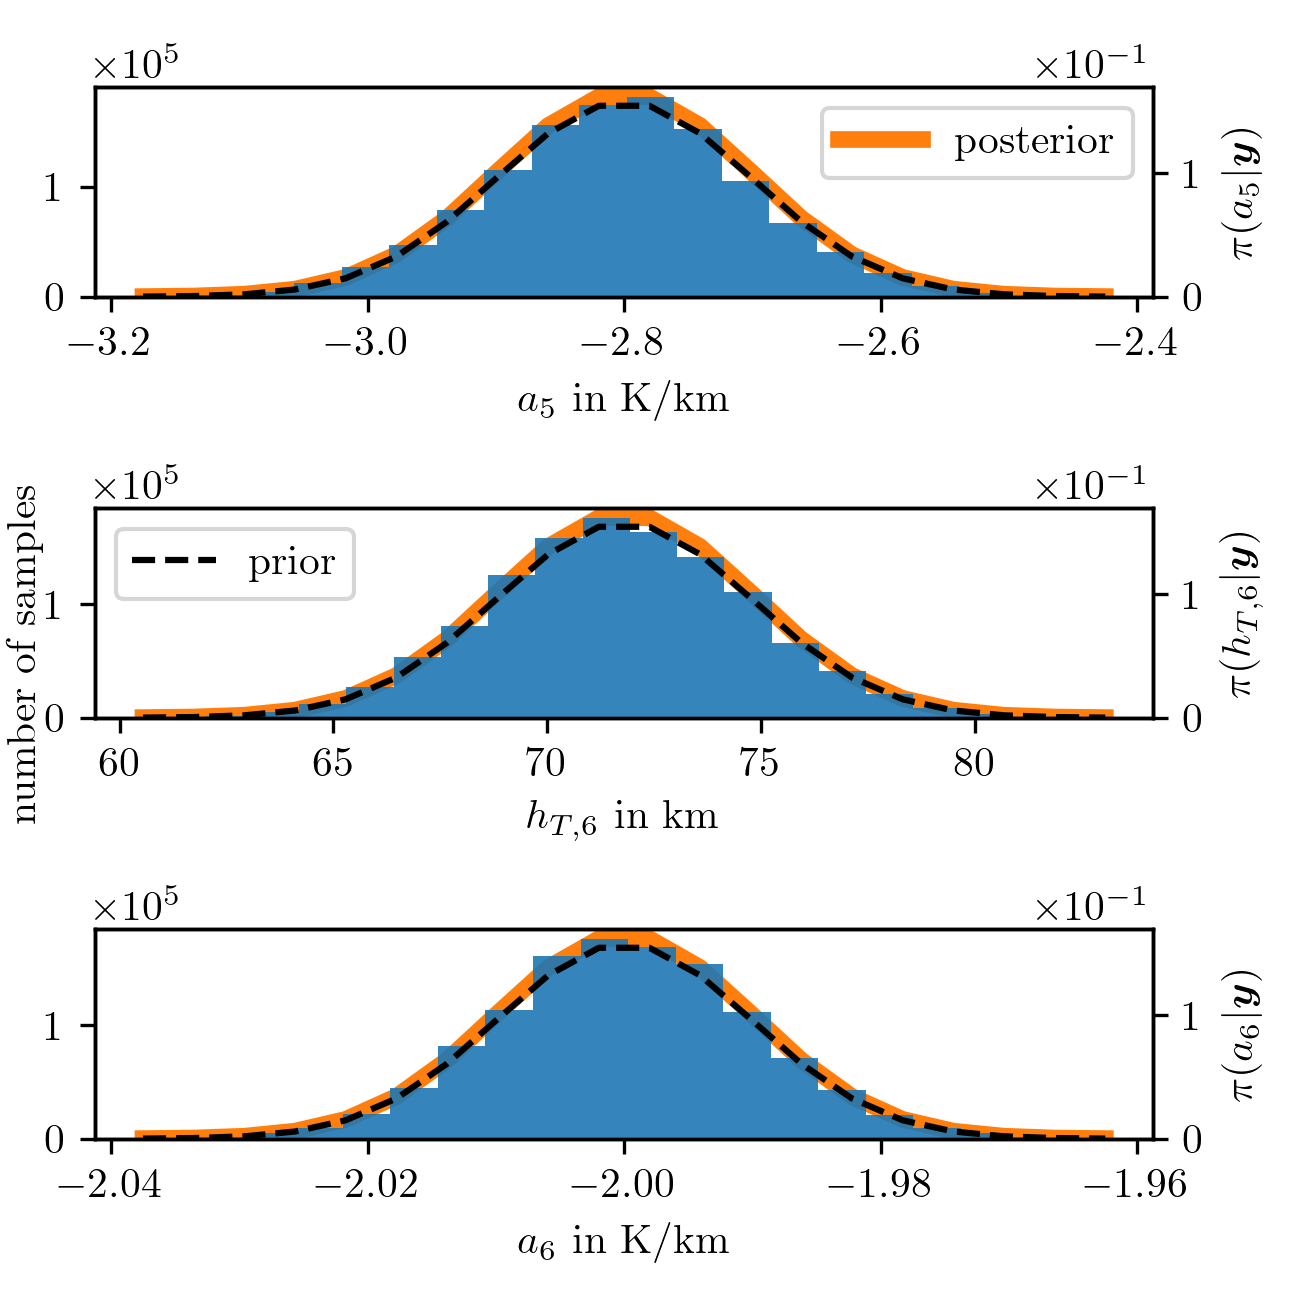
\includegraphics{PHdPTPost5.png}
	\caption[Histograms and TT approximation of posterior distribution as well as hyper-prior distribution.]{We plot the TT approximation of marginal posterior in orange and the samples as a histogram as well as the prior distribution with a dotted line.}
	\label{fig:PostHistTT5}
\end{figure}


We observe that the marginal do not differ significantly from the \texttt{t-walk} samples and report a relative RMS error between true and TT approximated function values at SIRT-MH samples of $\approx 7 \%$.
We report IATC for the SIRT-MH around $2-4$ and the IATC given in Tab. \ref{tab:priors}.
Additionally, we see when comparing the marginal posterior distributions to the prior distributions of the hyper-parameters that the hyper-parameter $b$ is the only hyper-parameter related to pressure and temperature which is affected by the data.
\clearpage


\subsubsection{Conditional Posterior Distribution}
We use the RTO method (see Sec. \ref{subsec:RTO}) to obtain ozone samples from the conditional posterior
To obtain posterior pressure and temperature samples take hyper-parameter samples directly from the marginal posterior.
Then we calculate pressure and temperature profile according to their respective function (see Eq. \ref{eq:pressFunc} and Eq. \ref{eq:tempFunc}). 
We plot the posterior temperature and pressure profiles in Fig. \ref{fig:TempPost} and Fig. \ref{fig:PressPost} and posterior ozone in \ref{fig:O3Post}.
\begin{figure}[ht!]
	\centering
	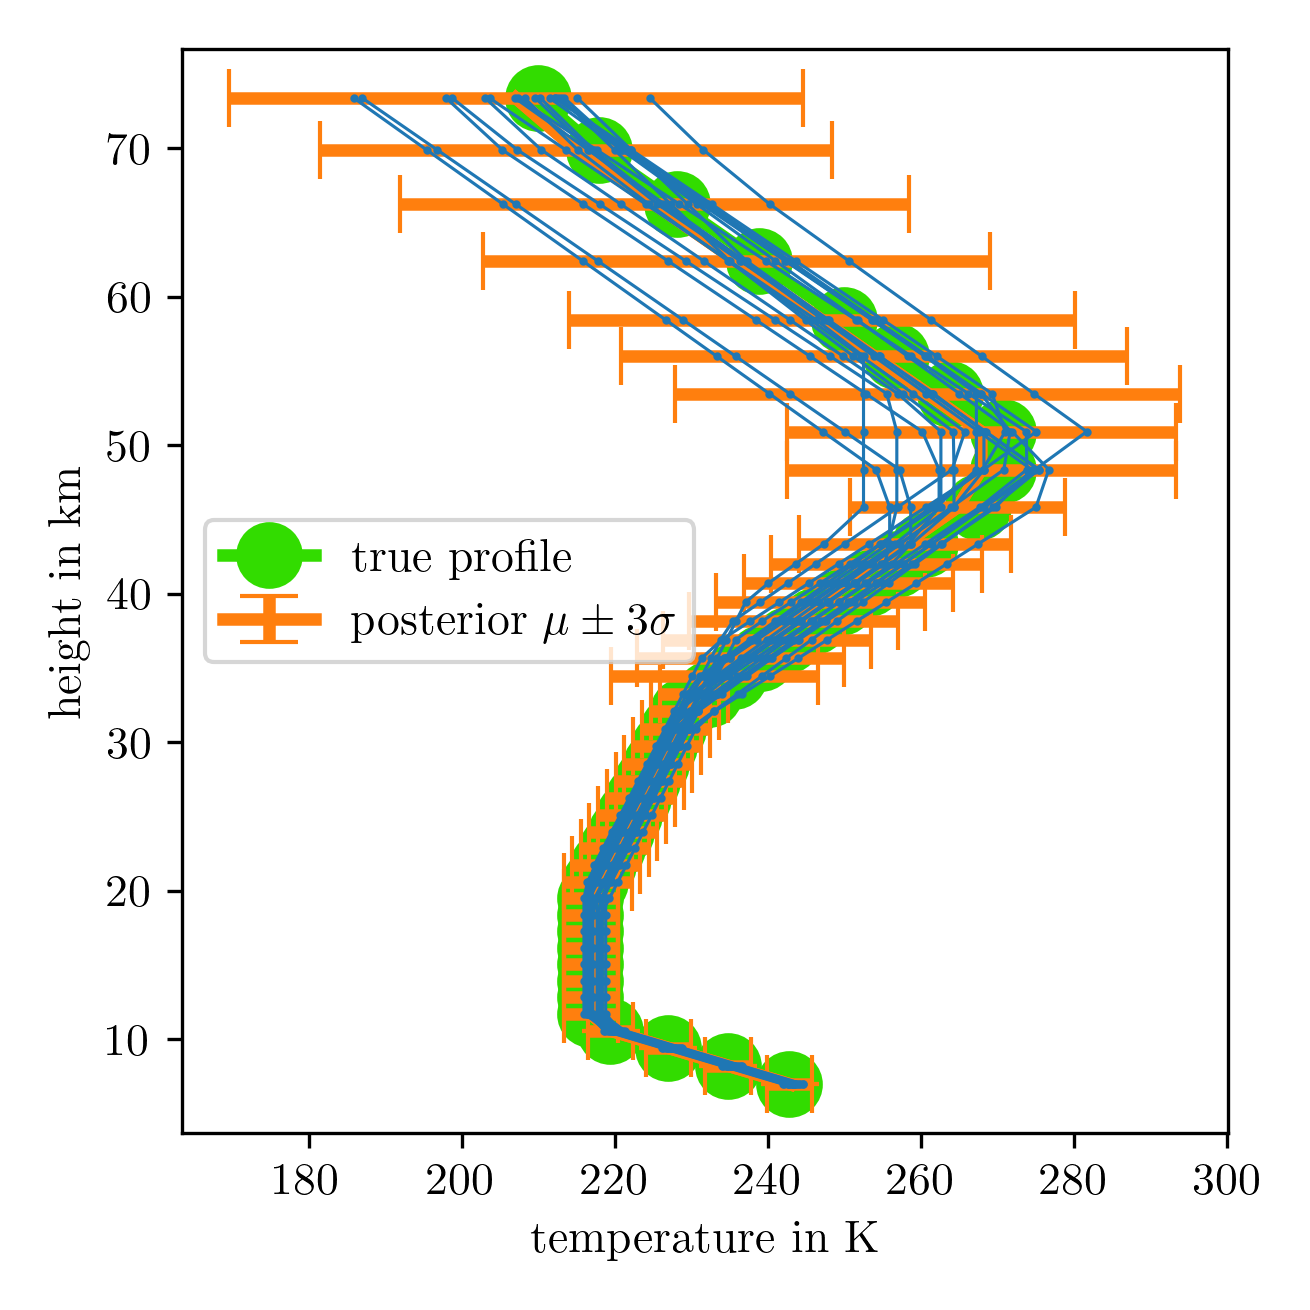
\includegraphics{TempPostMeanSigm.png} 
	\caption[Temperature posterior samples.]{We take samples from the posterior distribution, as plotted in Figures \ref{fig:PostHistTT0} to \ref{fig:PostHistTT3} and plot the corresponding temperature function, see Eq: \ref{eq:tempFunc}. }
	\label{fig:TempPost}
\end{figure}
\cleardoublepage
\begin{figure}[ht!]
	\centering
	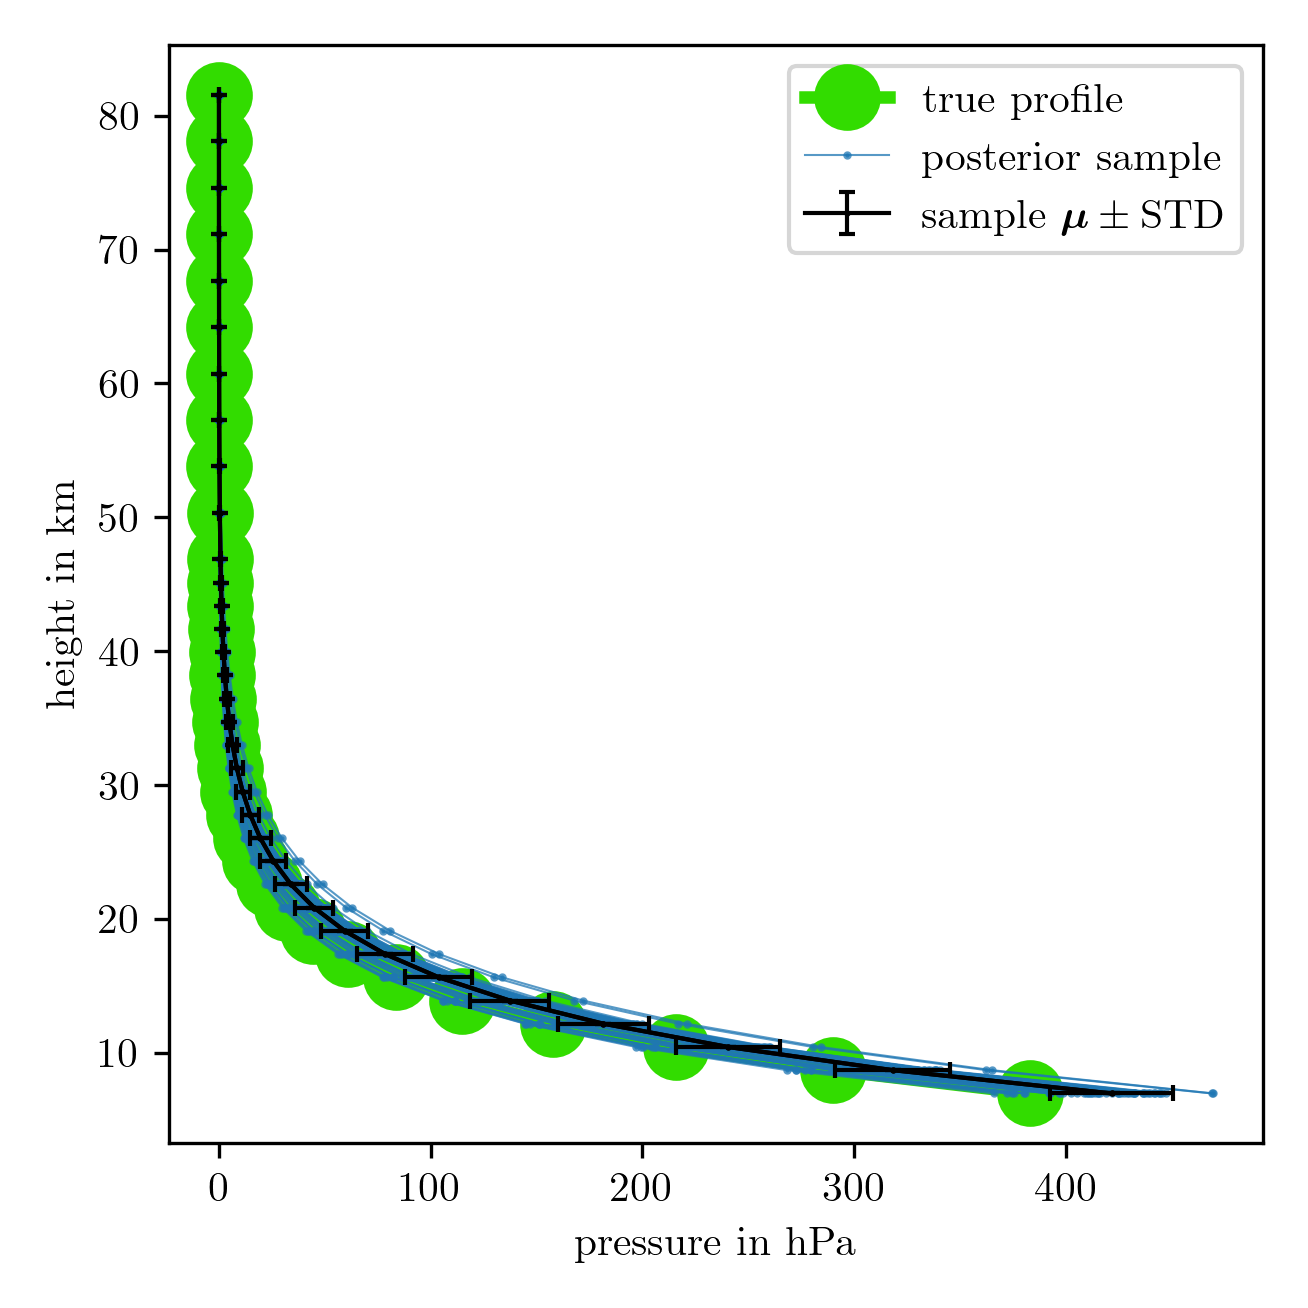
\includegraphics{PressPostMeanSigm.png}
	\caption[Pressure posterior samples.]{We take samples from the posterior distribution, as plotted in Fig. \ref{fig:PostHistTT4} and plot the corresponding pressure function, see Eq: \ref{eq:pressFunc}.}
	\label{fig:PressPost}
\end{figure}

\begin{figure}[ht!]
	\centering
	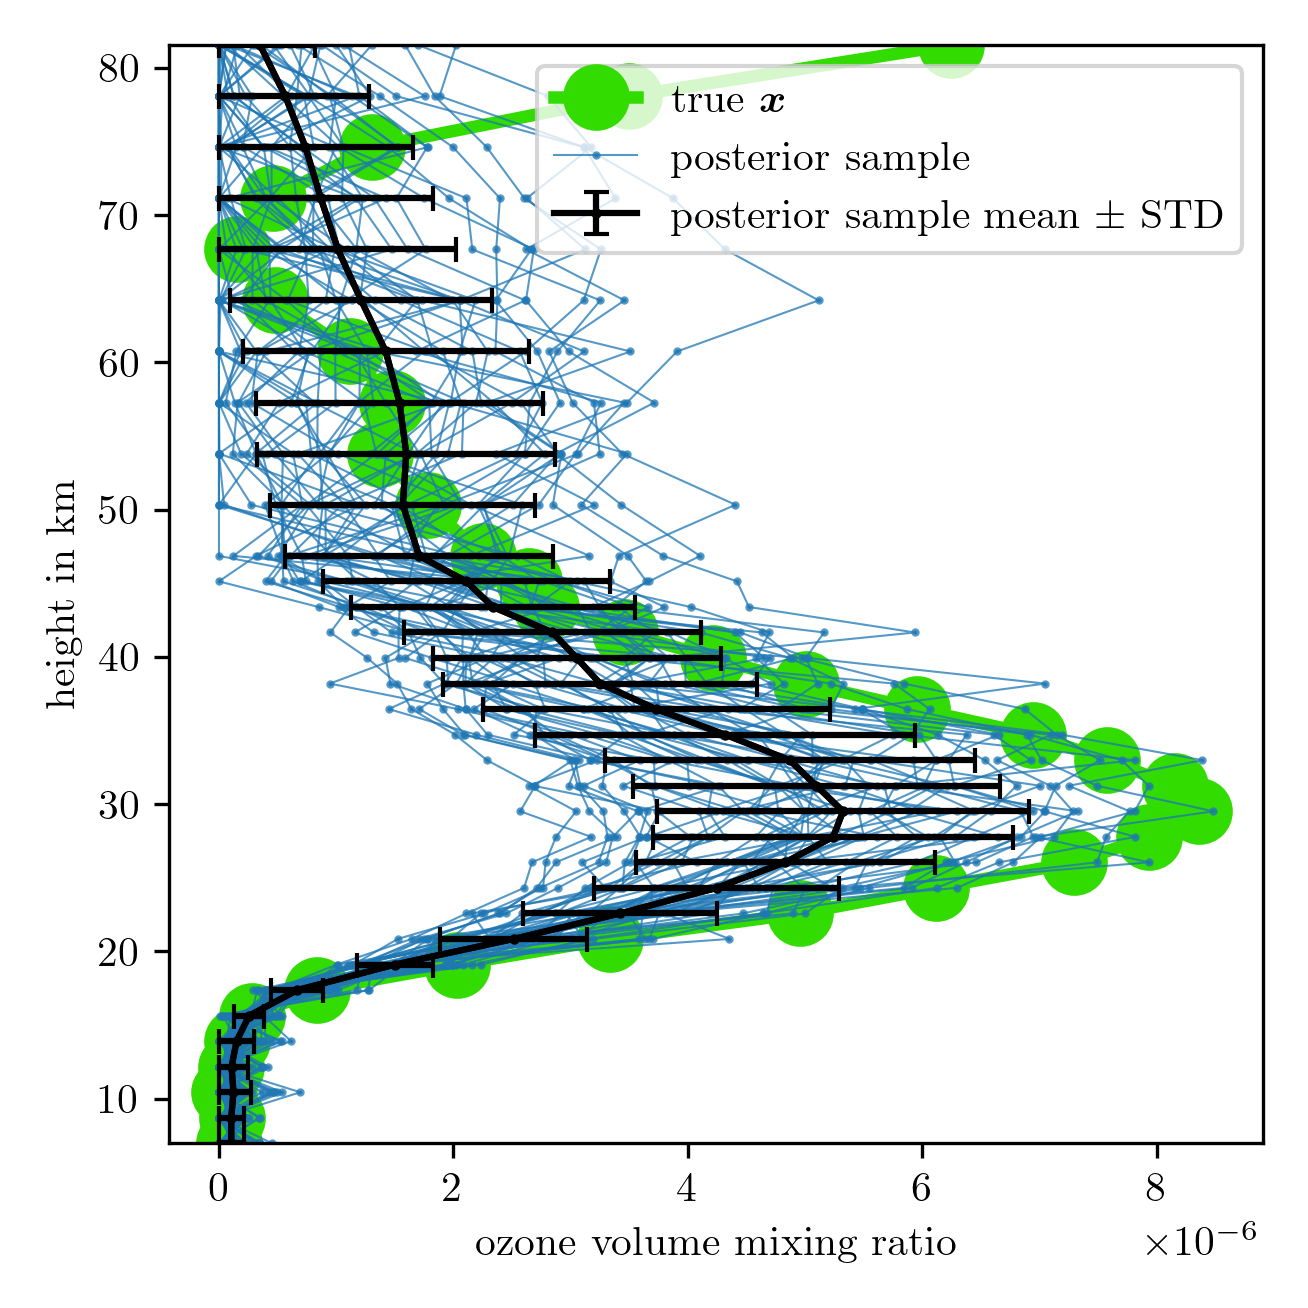
\includegraphics{FullO3Res.png}
	\caption[Pressure posterior samples.]{We take samples from the posterior distribution, as plotted in Fig. \ref{fig:PostHistTT4} and plot the corresponding pressure function, see Eq: \ref{eq:pressFunc}.}
	\label{fig:O3Post}
\end{figure}

We observe that pressure and ozone are highly correlated.
Since the hyper-parameter $b$ is smaller that the ground truth value the posterior pressure profile does not exponentially decrease as much compared the ground truth.
This results in posterior pressure values which are slightly larger than the ground truth.
In comparison, the corresponding posterior ozone profiles have much smaller individual ozone VMRs compared to the ground truth, but still a similar structure compared to the ground truth.
Again we are not able to recover the peak at large altitude.
\clearpage




%When approximating the marginal posterior the maximum relative propagation error $\underset{\lambda , \gamma}{\text{arg max}\,}|\tilde{\pi}(\lambda,\gamma|\bm{y}) - \pi(\lambda,\gamma|\bm{y}) |/ |\pi(\lambda,\gamma|\bm{y})|$ is approximately $100\%$ at $\gamma_{\text{max}}$ and $\lambda_{\text{max}}$, which are the maximum values of the $\lambda$ and $\gamma$ samples and lay in regions with very low probability.
%We consider this error negligible because the absolute error at $\gamma_{\text{max}}$ and $\lambda_{\text{max}}$ is smaller than $10^{-24} \approx 0$.
%Note that one can reduce the maximum errors when approximation $f(\lambda)$ at the mean of $\pi(\lambda,\gamma|\bm{y})$ instead of the modes since $\pi(\lambda | \bm{y})$ is skewed, but we don't see noticeable differences in the conditional posterior $\pi(\bm{x}|\lambda,\gamma,\bm{y})$ when doing so.
%We consider these errors as tolerable.
%$\lVert \pi(\bm{x}_{MH}) - \tilde{\pi}(\bm{x}_{MH}) \rVert / \lVert \pi(\bm{x}_{MH}) \rVert$
%$\lVert \mathbb{E}\big[ \bm{x} \big]  -  \mathbb{E} \big[ \tilde{\bm{x}} \big] \rVert_{L^2}$
%$\lVert \mathbb{E}  \big[\bm{x}\big] -  \mathbb{E} \big[ \bm{x}_{MH}\big]  \rVert_{L^2}$
%When we calculate the mean and covariance matrix of the full conditional $\pi(\bm{x}|\bm{y})$ we have to bin up the samples of the marginal posterior $\pi(\gamma, \delta |\bm{y})$ or use a TT approximation on a predefined grid with a certain number of grid points, we like to give an estimate for this error as well.
%In doing we bin up samples and use the height $\tilde{\pi}(\bm{\theta}^{(k)}_d)$ for a bin $k = 1, \dots, \text{N}_b$ to calculate the mean $\tilde{\mu}_d = \sum_{\text{N}_b} \tilde{\pi}(\bm{\theta}^{(k)}_d) $.
%We compare to the sample mean $\bm{\mu}_d = \sum_{k=1}^N \bm{\theta}^{(k)}_d/N$ and calculate the relative error $||\bm{\mu}_{\text{samp}} -\bm{\mu}_{\text{distr}} ||/ || \bm{\mu}_{\text{samp}} ||$
%where $\bm{\mu}_{\text{samp}} =(\tilde{\mu}_1, \dots , \tilde{\mu}_D) $ and equivalently $\bm{\mu}_{\text{distr}} =(\tilde{\mu}_1, \dots , \tilde{\mu}_D) $.
%Here $d$ refers to the $D = 16$ hyper-parameters $\gamma, \lambda, h_1, h_2, h_3, h_4, h_5, h_6, a_0, a_1, a_2, a_3, a_4, T_0, p_0, b$.




%\begin{figure}[thb!]
%	\centering
%	\begin{tikzpicture}
	%		
	%		\node[align=center] at (-1,4) (A)    {$\bm{M A}_L$};
	%		\node[roundnode2] at (-1,2.5) (u)    {$\bm{u}$};
	%		\node[rectnode] at (-1,1) (y)    {$\bm{y}$};
	%		
	%		\node[roundnode2] at (3,6.5) (t)     {$\bm{T}$};
	%		\node[roundnode2] at (-1,6.5) (p)     {$\bm{p}$};
	%		\node[roundnode2] at (1,5) (pt)     {$\bm{p}/\bm{T}$};
	%		\node[roundnode2] at (0,8) (b1)    {$b$};
	%		%\node[roundnode2] at (1,8) (b2)    {$b_2$};
	%		\node[roundnode2] at (-2,8) (h1)    {$h_0$};
	%		\node[roundnode2] at (-1,8) (p0)    {$p_0$};
	%		\node[roundnode2] at (2.25,8) (ht)    {$\bm{h}$};
	%		\node[roundnode2] at (3.25,8) (ct)    {$T_0$};
	%		\node[roundnode2] at (4.25,8) (at)    {$\bm{a}$};
	%		
	%		%Lines
	%		\draw[->, very thick] (u.south) -- (y.north);
	%		\draw[->, mydotted, very thick] (A.south) -- (u.north);
	%		
	%		\draw[->, mydotted, very thick] (p.south east) -- (pt.north west);
	%		\draw[->, mydotted, very thick] (t.south west) -- (pt.north east);
	%		\draw[->, mydotted, very thick] (pt.south west) -- (A.east);
	%		\draw[->, mydotted, very thick] (h1.south) -- (p.north west);
	%		\draw[->, mydotted, very thick] (p0.south) -- (p.north);
	%		\draw[->, mydotted, very thick] (b1.south) -- (p.north east); 
	%		%\draw[->, very thick] (b2.south) -- (p.east); 
	%		
	%		\draw[->, mydotted, very thick] (ht.south) -- (t.north west);
	%		\draw[->, mydotted, very thick] (ct.south) -- (t.north);
	%		\draw[->, mydotted, very thick] (at.south) -- (t.north east);
	%		
	%		\node[align =center] at (-5,8) (T1) {posterior \\ over hyper-parameters \\ $\pi(h_0, p_0, b, \bm{h}, T_0, \bm{a}| \bm{y})$};
	%		
	%		\node[fit=(h1)(at),draw,dotted,black, rounded corners] {};
	%	\end{tikzpicture} 
%	\caption[Directed acyclic Graph for pressure and temperature.]{Conditioned on an ozone profile the posterior of the hyper-parameters describing pressure and temperature is given as in Eq. \ref{eq:}. Since pressure and temperature go into the forward model as $\bm{p}/\bm{T}$ they are highly correlated but the pressure is the dominant parameter, see Fig. 
	%		\ref{fig:PriorPressOverTemp} and \ref{fig:SeaLevelHist}. Note that here we use the updated forward model $\bm{M} \bm{A}_L$ and conditioned on a $\gamma$ sample from the previously evaluated marginal posterior see Fig. \ref{fig:MargPostHistTT}. }
%	\label{fig:DAGPT}
%\end{figure}